\section{Consuntivo}
		In questa sezione verranno riportati il consuntivo per le varie fasi di lavoro, considerando le ore sostenute da ogni componente per ruolo. Il bilancio potrà essere:
		\begin{itemize}
			\item \textbf{positivo:} se sono state necessarie meno ore rispetto a quelle preventivate;	 
			\item \textbf{paritario:} se le ore preventivate rispettano quelle effettive;	 
			\item \textbf{negativo:} se sono state necessarie più ore rispetto a quelle preventivate.
		\end{itemize}
	\subsection{Fase di analisi dei requisiti}
		Le ore di lavoro svolto in questo periodo sono di solo investimento e destinate all'apprendimento personale. Di conseguenza queste ore non sono rendicontate. 
		\subsubsection{Prospetto orario}
			Nella tabella in seguito viene illustrato il cambiamento nel numero d'ore di ogni persona, per ogni ruolo ricoperto:
			
			\rowcolors{2}{white}{lightest-grayest}
			\begin{longtable}{|l|c|c|c|c|c|c|c|}
				\hline
				\rowcolor{lighter-grayer}
				\textbf{Nome} & \textbf{Re} & \textbf{Am} & \textbf{An} & \textbf{Pg}  & \textbf{Pr}   & \textbf{Ve} & \textbf{Totale} \\
				\hline
				\endfirsthead
				
				\hline
				Giuseppe Vito Bitetti 		& 0 & 8(-1) & 10(+1) & 0 & 0 & 12 & 30\\
				\hline
				\hline
				Lorenzo Dei Negri			 & 6(-2) & 0 & 14(+1) & 0 & 0 & 10(+1) & 30\\
				\hline
				\hline
				Nicolò Frison 					& 0 & 8(-2) & 9(+1) & 0 & 0 & 13(+1) & 30\\
				\hline
				\hline
				Fouad Mouad 				& 0 & 7 & 11 & 0 & 0 & 12 & 30\\
				\hline
				\hline
				Mariano Sciacco 			& 8 & 0 & 12 & 0 & 0 & 10 & 30\\
				\hline
				\hline
				Alessandro Tommasin    & 9(-2) & 0 & 12(+2) & 0 & 0 & 9 & 30\\
				\hline
				\hline
				Giovanni Vidotto 			& 0 & 6(-1) & 9(+1) & 0 & 0 & 15 & 30\\
				\hline 
				\caption{Tabella consuntiva contenente il prospetto orario per la fase di analisi dei requisiti}
			\end{longtable}
			\pagebreak	
			
			La tabella può essere riassunta nel seguente istogramma:
			
			\begin{figure}[H]
				\centering
				\includegraphics[width=0.8\linewidth]{images/consuntivo/analisiCons1.png}
				\caption{Diagramma consuntivo ore/ruolo componenti nella fase di analisi dei requisiti}
				\label{fig:consuntivo diagramma suddivisione ruoli fase analisi dei requisiti}
			\end{figure}
			
		\subsubsection{Prospetto economico}
			In base al prospetto orario, quello economico sarà il seguente: 
			
			\rowcolors{2}{white}{lightest-grayest}
			\begin{longtable}{|l|c|c|c|c|c|c|c}
				\hline
				\rowcolor{lighter-grayer}
				\textbf{Ruolo} & \textbf{Ore} & \textbf{Costo in €} \\
				\hline
				\endfirsthead
				
				\hline
				Responsabile & 23 (-4) & 690,00 (-120,00)\\
				\hline
				\hline
				Amministratore & 29 (-4) & 580,00 (-80,00)\\
				\hline
				\hline
				Analista & 77 (+6) & 1.925,00 (+150,00)\\
				\hline
				\hline
				Progettista & - & -\\
				\hline
				\hline
				Programmatore & - & -\\
				\hline
				\hline
				Verificatore & 81 (+2) & 1.215,00 (+30,00)\\
				\hline
				\textbf{Totale} & 210 & 4.410,00 (-20,00)\\
				\hline
				\caption{Tabella contenente il prospetto economico in riferimento al prospetto orario}
			\end{longtable}
			\pagebreak
			
			La tabella può essere riassunta nel seguente areogramma:
			\begin{figure}[H]
				\centering
				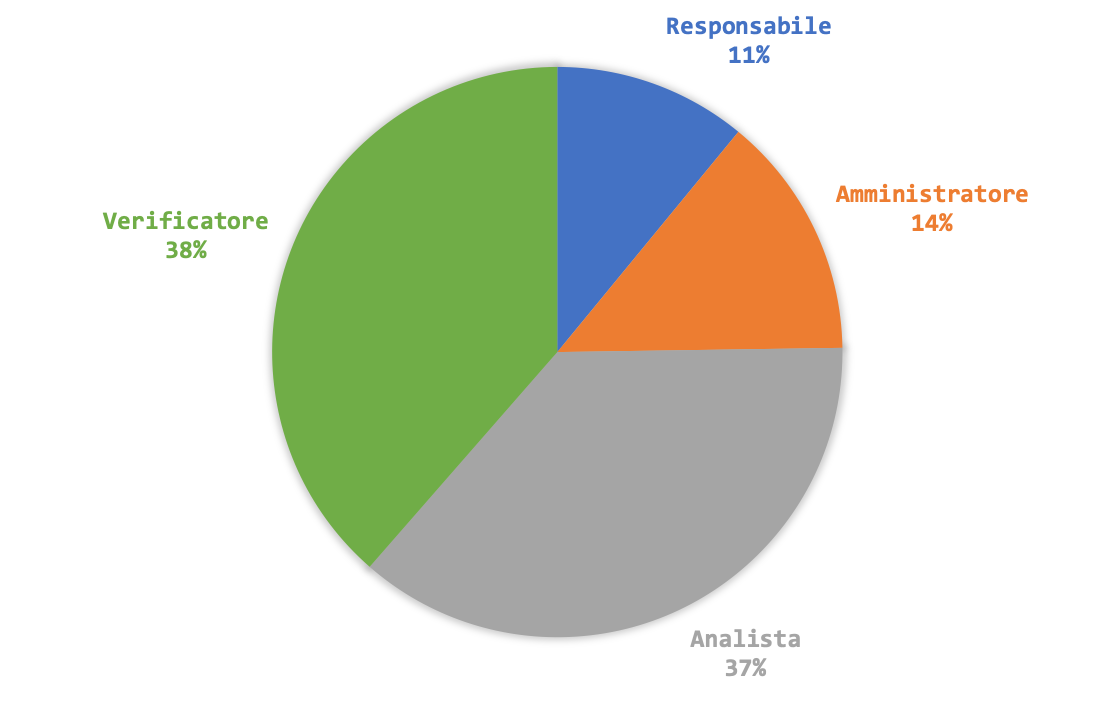
\includegraphics[width=0.8\linewidth]{images/consuntivo/analisiCons2.png}
				\caption{Diagramma percentuale ore/ruolo nella fase di analisi dei requisiti}
				\label{fig:consuntivo2 diagramma costi ruolo fase analisi dei requisiti}
			\end{figure}
		\subsubsection{Conclusioni}
			In questa fase il gruppo ha investito lo stesso numero di ore che erano state preventivate, applicando però delle correzioni per quanto riguarda l'assegnazione oraria per i diversi ruoli:
			\begin{itemize}
				\item \textbf{responsabile:} sono state impiegate meno ore rispetto a quelle preventivate in quanto nella pianificazione del lavoro e nella stesura del piano di progetto sono state riscontrate meno difficoltà del previsto;	 
				\item \textbf{amministratore:} dal momento che i software per la gestione del progetto sono stati individuati e configurati fin da subito e che i documenti sono stati ben strutturati in poco tempo, anche in questo caso sono state impiegate meno ore rispetto a quelle preventivate;
				\item \textbf{analista:} il ruolo di analista ha richiesto alcune ore in più del preventivato in quanto alcuni requisiti hanno richiesti più ore per essere compresi in maniera esaustiva;
				\item \textbf{verificatore:} le ore in surplus che sono state risparmiate dal responsabile e non ancora utilizzate dagli analisti sono state impiegate per effettuare una verifica più attenta dei documenti.  
			\end{itemize}
		\subsubsection{Preventivo a finire}
			Nonostante alcuni ruoli abbiano subito dei cambiamenti orari, il totale delle ore è rimasto invariato, di conseguenza il preventivo a finire resta in linea con quanto dichiarato in \S5. Inoltre, gli scostamenti dal preventivo non richiedono interventi di mitigazione in quanto la fase di analisi non è rendicontata.

		\subsection{Fase di consolidamento dei requisiti}
		Le ore di lavoro svolte in questo periodo sono volte alla preparazione della presentazione e alla revisione dei requisiti individuati. 
		\subsubsection{Prospetto orario}
			Nella tabella in seguito viene illustrato il cambiamento nel numero d'ore di ogni persona, per ogni ruolo ricoperto:
			
			\rowcolors{2}{lightest-grayest}{white}
			\begin{longtable}{|l|c|c|c|c|c|c|c|}
				\hline
				\rowcolor{lighter-grayer}
				\textbf{Nome} & \textbf{Re} & \textbf{Am} & \textbf{An} & \textbf{Pg}  & \textbf{Pr}   & \textbf{Ve} & \textbf{Totale} \\
				\hline
				\endfirsthead
				
				\hline
				Giuseppe Vito Bitetti 	& 0 & 0 & 5 & 0 & 0 & 0 & 5\\
				\hline
				\hline
				Lorenzo Dei Negri	 	& 0 & 5 & 0 & 0 & 0 & 0 & 5\\
				\hline
				\hline
				Nicolò Frison			   & 0 & 0 & 0 & 0 & 0 & 5 & 5\\
				\hline
				\hline
				Fouad Mouad 			& 1 (-1) & 0 & 1 (+1) & 0 & 0 & 3 & 5\\
				\hline
				\hline
				Mariano Sciacco		 	& 0 & 0 & 3 & 0 & 0 & 2 & 5\\
				\hline
				\hline
				Alessandro Tommasin & 0 & 0 & 5 (+1) & 0 & 0 & 0 (-1) & 5\\
				\hline
				\hline
				Giovanni Vidotto 		 & 2 & 0 & 0 & 0 & 0 & 3 & 5\\
				\hline 
				\textbf{Totale} 			& 3 (-1) &  5 & 14 (+2) & 0 & 0 & 13 (-1) & 35\\
				\hline
				\caption{Tabella consuntiva contenente il prospetto orario per la fase di consolidamento dei requisiti}
			\end{longtable}
			
			La tabella può essere riassunta nel seguente istogramma:
			
			\begin{figure}[H]
				\centering
				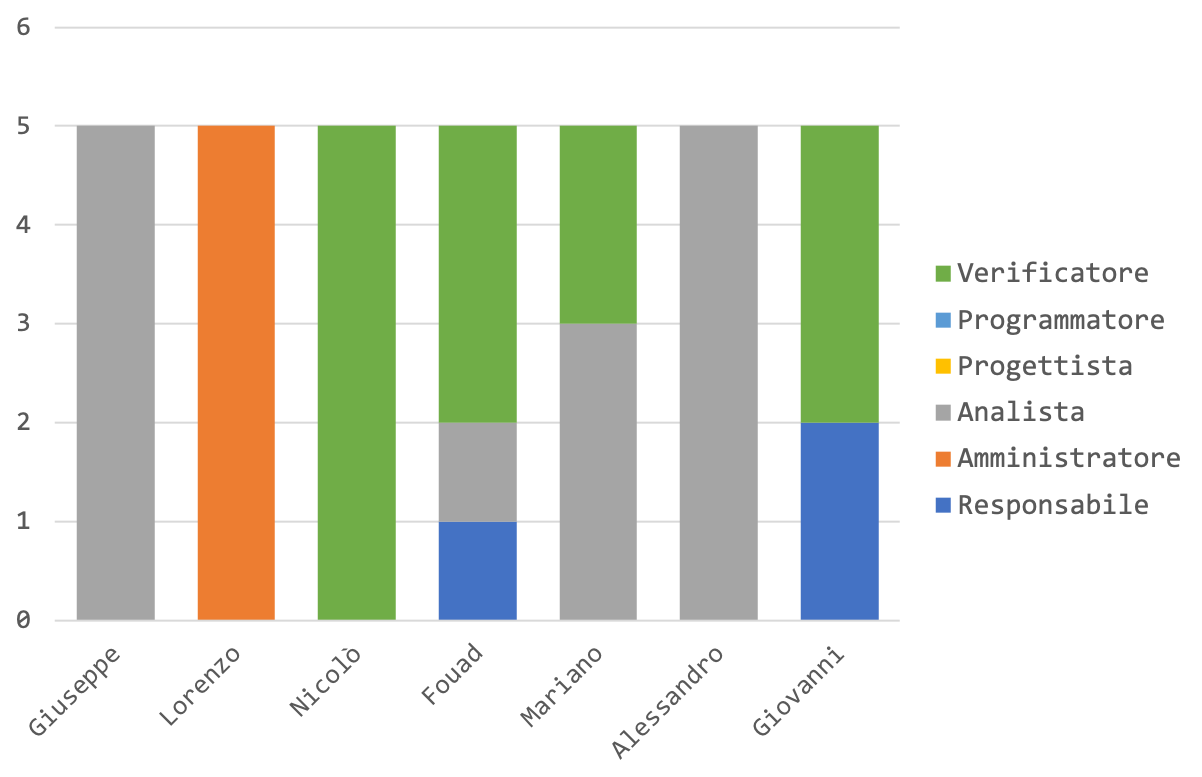
\includegraphics[width=0.8\linewidth]{images/consuntivo/ConsReqCons.png}
				\caption{Diagramma consuntivo ore/ruolo componenti della fase di consolidamento dei Requisiti}
				\label{fig:consuntivo diagramma suddivisione ruoli fase di consolidamento dei requisiti}
			\end{figure}
			
		\subsubsection{Prospetto economico}
			In base al prospetto orario, quello economico sarà il seguente: 
			
			\rowcolors{2}{white}{lightest-grayest}
			\begin{longtable}{|l|c|c|c|c|c|c|c|}
				\hline
				\rowcolor{lighter-grayer}
				\textbf{Ruolo} & \textbf{Ore} & \textbf{Costo in €} \\
				\hline
				\endfirsthead
				
				\hline
				Responsabile & 3 (-1) & 90,00 (-30,00)\\
				\hline
				\hline
				Amministratore & 5 & 100,00\\
				\hline
				\hline
				Analista & 14 (+2) & 350,00 (+50,00)\\
				\hline
				\hline
				Progettista & - & -\\
				\hline
				\hline
				Programmatore & -  & -\\
				\hline
				\hline
				Verificatore & 13 (-1) & 195,00 (-15,00)\\
				\hline
				\textbf{Totale} & 35 & 735,00 (+5,00)\\
				\hline
				\caption{Tabella contenente il prospetto economico in riferimento al prospetto orario}
			\end{longtable}
			
			La tabella può essere riassunta nel seguente areogramma:
			\begin{figure}[H]
				\centering
				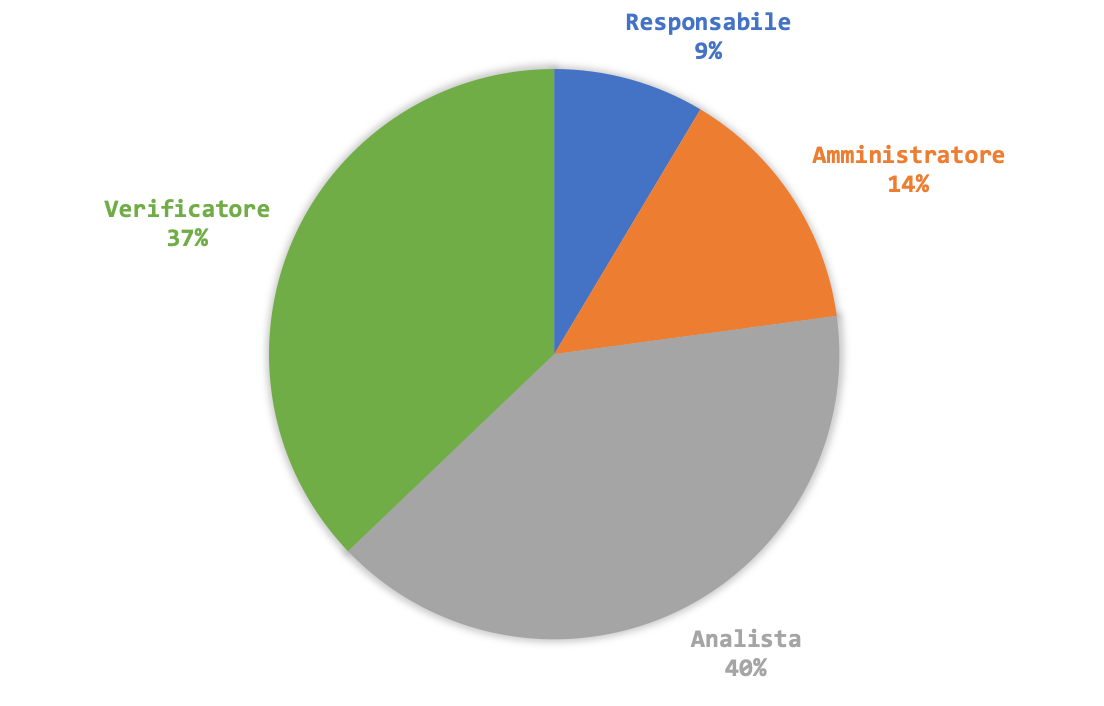
\includegraphics[width=0.8\linewidth]{images/consuntivo/ConsReqCons2.png}
				\caption{Diagramma percentuale ore/ruolo nella fase di consolidamento dei requisiti}
				\label{fig:consuntivo diagramma costi ruolo fase di consolidamento dei requisiti}
			\end{figure}
		
		\subsubsection{Conclusioni }
			In questa fase il gruppo ha investito il numero di ore che erano state preventivate. È stato necessario però svolgere alcuni cambiamenti nella suddivisione oraria per ruolo, in particolare:
			\begin{itemize}
				\item \textbf{responsabile:} il ruolo di responsabile ha richiesto alcune ore in meno in quanto l'approvazione dei documenti e la redazione delle sezioni sono state meno complesse di ciò che era stato preventivato;
				\item \textbf{analista:} per questo ruolo è stato necessario spendere qualche ora in più in quanto alcuni requisiti, per una corretta comprensione, hanno richiesto una delucidazione esterna con i proponenti del progetto, avvenuta con alcune difficoltà di comunicazione;
				\item \textbf{verificatore:} poiché il lavoro degli analisti è stato svolto con precisione, il lavoro dei verificatori è stato leggermente più veloce di ciò che era stato preventivato.
			\end{itemize}
			Alla luce dei cambiamenti effettuati il risultato è che il gruppo ha risparmiato in totale € 15,00 investendo le stesse ore preventivate.
		\subsubsection{Preventivo a finire}
			Il preventivo a finire non modifica quanto preventivato in \S5 in quanto, al netto di alcune ridistribuzioni orarie, il monte ore previsto per questa fase è stato rispettato.
		\pagebreak

		\subsection{Fase di progettazione della technology baseline}
		Le ore di lavoro svolte in questo periodo sono volte alla progettazione della \textit{technology baseline} e alla realizzazione della \glock{proof of concept}. 

		\subsubsection{Prospetto orario}
			Nella tabella in seguito viene illustrato il cambiamento nel numero d'ore di ogni persona, per ogni ruolo ricoperto:
			
			\rowcolors{2}{lightest-grayest}{white}
			\begin{longtable}{|l|c|c|c|c|c|c|c|}
				\hline
				\rowcolor{lighter-grayer}
				\textbf{Nome} & \textbf{Re} & \textbf{Am} & \textbf{An} & \textbf{Pg}  & \textbf{Pr}   & \textbf{Ve} & \textbf{Totale} \\
				\hline
				\endfirsthead
				\hline
				Giuseppe Vito Bitetti & 2 (-1) & 0 & 7 & 0 & 0 & 4 (+1) & 13\\
				\hline
				\hline
				Lorenzo Dei Negri & 0 & 5 & 1 & 5 & 0 & 2 & 13\\
				\hline
				\hline
				Nicolò Frison & 0 & 3 & 5 & 5 & 0 & 0 & 13\\
				\hline
				\hline
				Fouad Mouad & 0 & 4 & 3 & 2 & 0 & 4 & 13 \\
				\hline
				\hline
				Mariano Sciacco & 3 & 0 & 1 & 9 & 0 & 0 & 13\\
				\hline
				\hline
				Alessandro Tommasin & 0 & 4 & 6 & 0 & 0 & 3  & 13\\
				\hline
				\hline
				Giovanni Vidotto & 2 & 0 & 5 & 2 & 0 & 4 & 13\\
				\hline 
				\textbf{Totale} & 7 (-1) &  16 & 28 & 23 & 0 & 17 (+1) & 91 \\
				\hline
				
				\caption{Tabella consuntiva contenente il prospetto orario per la fase di progettazione della technology baseline}
			\end{longtable}
			
			La tabella può essere riassunta nel seguente istogramma:
			
			\begin{figure}[H]
				\centering
				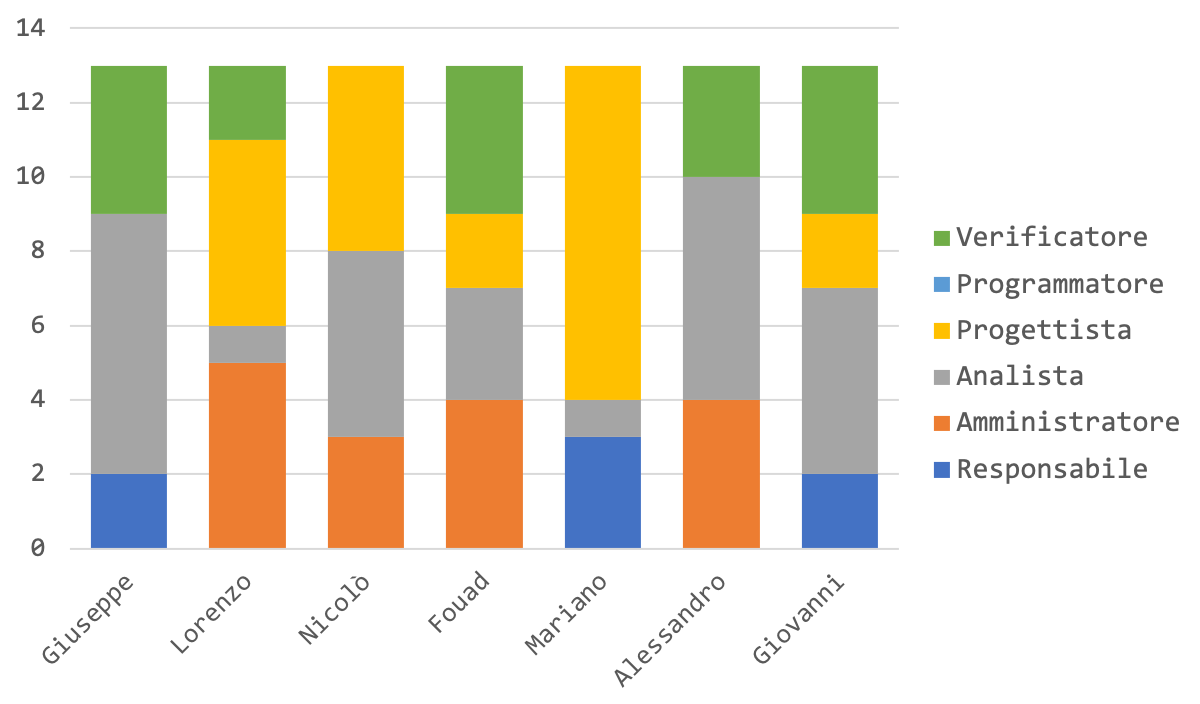
\includegraphics[width=0.8\linewidth]{images/consuntivo/ConsCorrez1.png}
				\caption{Diagramma consuntivo ore/ruolo componenti della fase di progettazione della technology baseline}
				\label{fig:consuntivo diagramma suddivione ruoli fase di progettazione della technology baseline}
			\end{figure}
		\pagebreak
			
		\subsubsection{Prospetto economico}
			In base al prospetto orario, quello economico sarà il seguente: 
			
			\rowcolors{2}{white}{lightest-grayest}
			\begin{longtable}{|l|c|c|c|c|c|c|c}
				\hline
				\rowcolor{lighter-grayer}
				\textbf{Ruolo} & \textbf{Ore} & \textbf{Costo in €} \\
				\hline
				\endfirsthead
				\hline
				Responsabile 	    & 7 (-1) & 210,00 (-30,00)\\
				\hline 
				\hline
				Amministratore	  & 16 & 320,00\\
				\hline
				\hline
				Analista 				& 28 & 700,00\\
				\hline
				\hline
				Progettista 		  & 23 & 506,00\\
				\hline
				\hline
				Programmatore 	 & 0 & 0,00\\
				\hline
				\hline
				Verificatore 		  & 17 (+1) & 255,00 (+15,00)\\
				\hline
				\textbf{Totale} 	& 91 & 1.991 (-15,00)\\
				\hline
				
				\caption{Tabella contenente il prospetto economico in riferimento al prospetto orario}
			\end{longtable}
			
			La tabella può essere riassunta nel seguente areogramma:
			\begin{figure}[H]
				\centering
				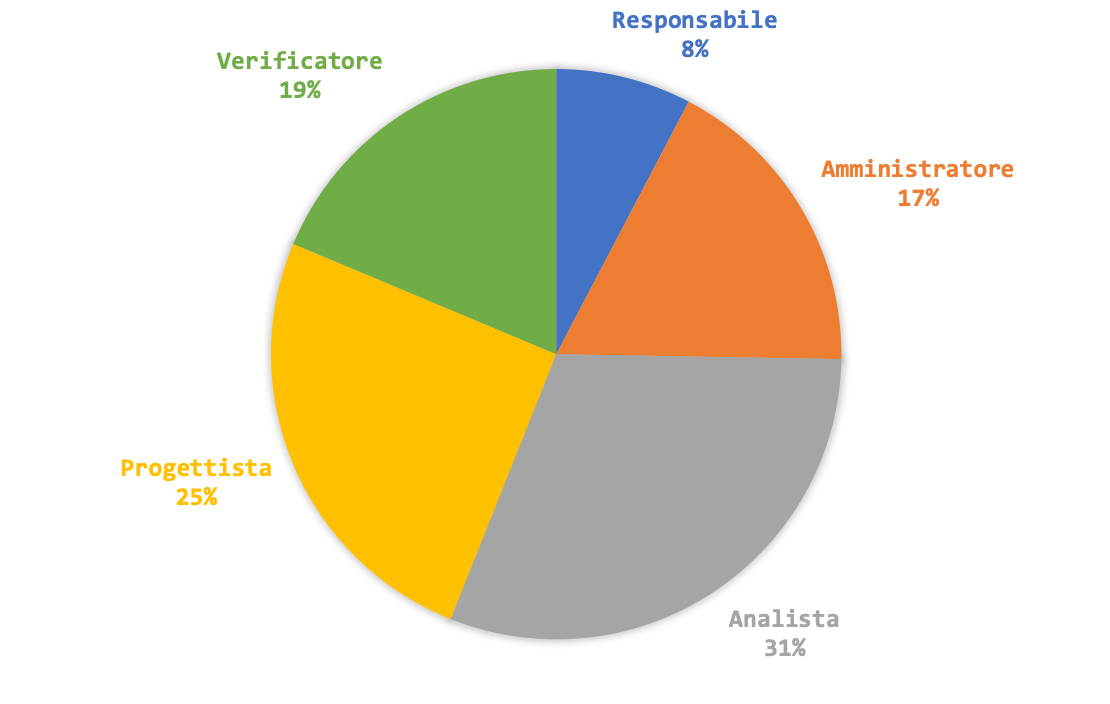
\includegraphics[width=0.8\linewidth]{images/consuntivo/ConsCorrez2.png}
				\caption{Diagramma percentuale ore/ruolo nella fase di progettazione della technology baseline}
				\label{fig:consuntivo diagramma costi ruolo fase progettazione della technology baseline}
			\end{figure}

		\subsubsection{Conclusioni}
			Durante la fase di progettazione della technology baseline il gruppo ha lavorato mantenendo il numero di ore che erano state preventivate. È stato necessario però svolgere alcuni cambiamenti nella suddivisione oraria per ruolo, in particolare:
			\begin{itemize}
				\item \textbf{responsabile:} il ruolo del responsabile è stato svolto più velocemente di ciò che era stato preventivato richiedendo quindi un'ora in meno;
				\item \textbf{verificatore:} si è deciso di aggiungere un'ora di verifica aggiuntiva per ricontrollare il piano di progetto e il piano di qualifica, alla luce delle modifiche fatte in seguito alle osservazioni del committente.
			\end{itemize}
			Alla luce dei cambiamenti effettuati il risultato è che il gruppo ha risparmiato € 15,00 investendo le stesse ore preventivate.
		
		\subsubsection{Preventivo a finire}
			A seguito dei recenti cambiamenti apportati alla pianificazione, nonostante alcune lievi modifiche all'assegnazione oraria dei ruoli per la fase corrente, e tenendo in considerazione il leggero risparmio maturato, da parte del committente, sul costo totale del progetto, è stato deciso di non intervenire sul preventivo.	
			
		\subsection{Progettazione e codifica del Proof of Concept e funzionalità essenziali}
		Vedremo in dettaglio i consuntivi dei successivi quattro incrementi, che compongono la fase stessa.  	
			
		\subsubsection{Incremento I}
		Le ore di lavoro svolte in questo periodo sono volte alla configurazione dei container e dell'immagine \glock{Docker} di Kafka. 
		\paragraph{Prospetto orario}
			Nella tabella in seguito viene illustrato il cambiamento nel numero d'ore di ogni persona, per ogni ruolo ricoperto:
			
			\rowcolors{2}{lightest-grayest}{white}
			\begin{longtable}{|l|c|c|c|c|c|c|c|}
				\hline
				\rowcolor{lighter-grayer}
				\textbf{Nome} & \textbf{Re} & \textbf{Am} & \textbf{An} & \textbf{Pg}  & \textbf{Pr}   & \textbf{Ve} & \textbf{Totale} \\
				\hline
				\endfirsthead
				\hline
				Giuseppe Vito Bitetti & 0 & 0 & 3 & 0 & 2 & 0 & 5\\
				\hline
				\hline
				Lorenzo Dei Negri & 0 & 0 & 0 & 1 (-1) & 0 & 4 (+1) & 5\\
				\hline
				\hline
				Nicolò Frison & 0 & 2 (-1) & 0 & 0 & 0 & 3(+1) & 5\\
				\hline
				\hline
				Fouad Mouad & 3 & 0 & 2 & 0 & 0 & 0 & 5\\
				\hline
				\hline
				Mariano Sciacco & 0 & 0 & 0 & 3 & 2 & 0 & 5\\
				\hline
				\hline
				Alessandro Tommasin & 0 & 2 & 0 & 3 & 0 & 0 & 5\\
				\hline
				\hline
				Giovanni Vidotto & 2 & 0 & 0 & 0 & 4 & 1 & 5\\
				\hline 
				\textbf{Totale} & 3 &  4 (-1) & 5 & 7 (-1) & 8 & 8 (+2) & 35\\
				\hline 
				
				\caption{Tabella consuntiva contenente il prospetto orario per l'incremento I}
			\end{longtable}
			\pagebreak
			
			La tabella può essere riassunta nel seguente istogramma:
			
			\begin{figure}[H]
				\centering
				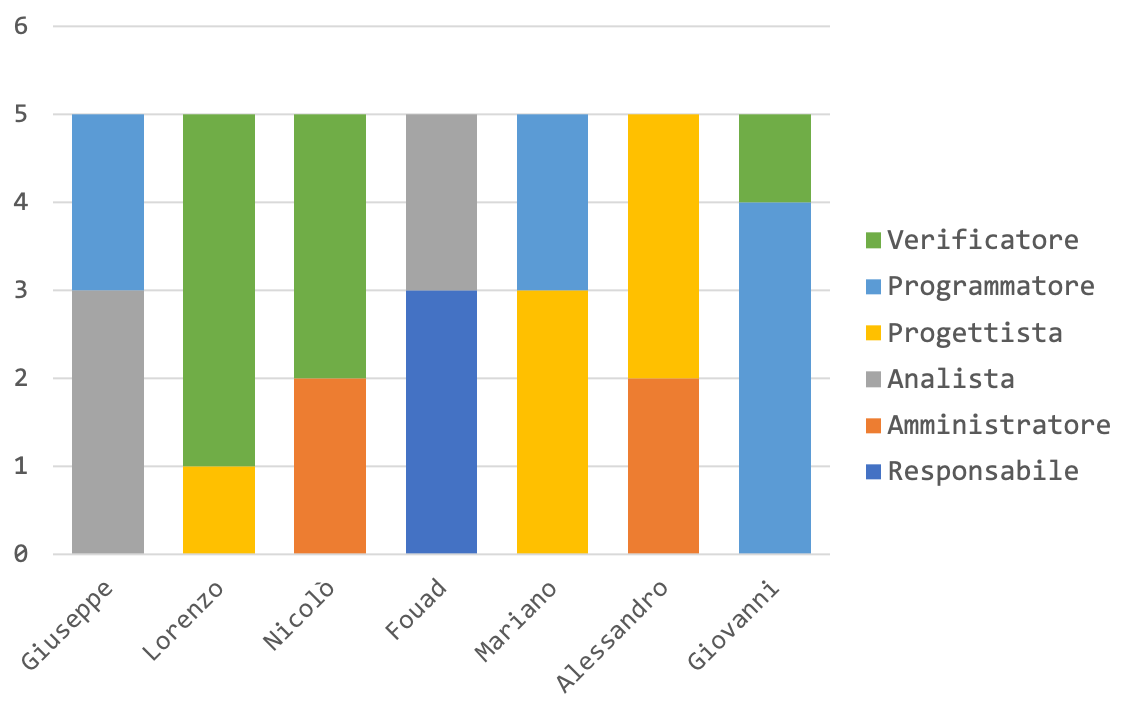
\includegraphics[width=0.8\linewidth]{images/consuntivo/ConsIncr1-1.png}
				\caption{Diagramma consuntivo ore/ruolo componenti dell'incremento I}
				\label{fig:consuntivo diagramma suddivione ruoli incremento I}
			\end{figure}
			
		\paragraph{Prospetto economico}
			In base al prospetto orario, quello economico sarà il seguente: 
			
			\rowcolors{2}{white}{lightest-grayest}
			\begin{longtable}{|l|c|c|c|c|c|c|c|}
				\hline
				\rowcolor{lighter-grayer}
				\textbf{Ruolo} & \textbf{Ore} & \textbf{Costo in €} \\
				\hline
				\endfirsthead
				\hline
			Responsabile 	    & 3 & 90,00\\
			\hline 
			\hline
			Amministratore	  & 4 (-1)& 80,00 (-20,00)\\
			\hline
			\hline
			Analista 				& 5 & 125,00\\
			\hline
			\hline
			Progettista 		  & 7 (-1) & 154,00 (-22,00)\\
			\hline
			\hline
			Programmatore 	 & 8 & 120,00\\
			\hline
			\hline
			Verificatore 		  & 8 (+2) & 120,00 (+30,00)\\
			\hline
			\textbf{Totale} 	& 35 & 689,00 (-12,00)\\
			\hline
				
				\caption{Tabella contenente il prospetto economico in riferimento al prospetto orario}
			\end{longtable}
		\pagebreak
			
			La tabella può essere riassunta nel seguente areogramma:
			\begin{figure}[H]
				\centering
				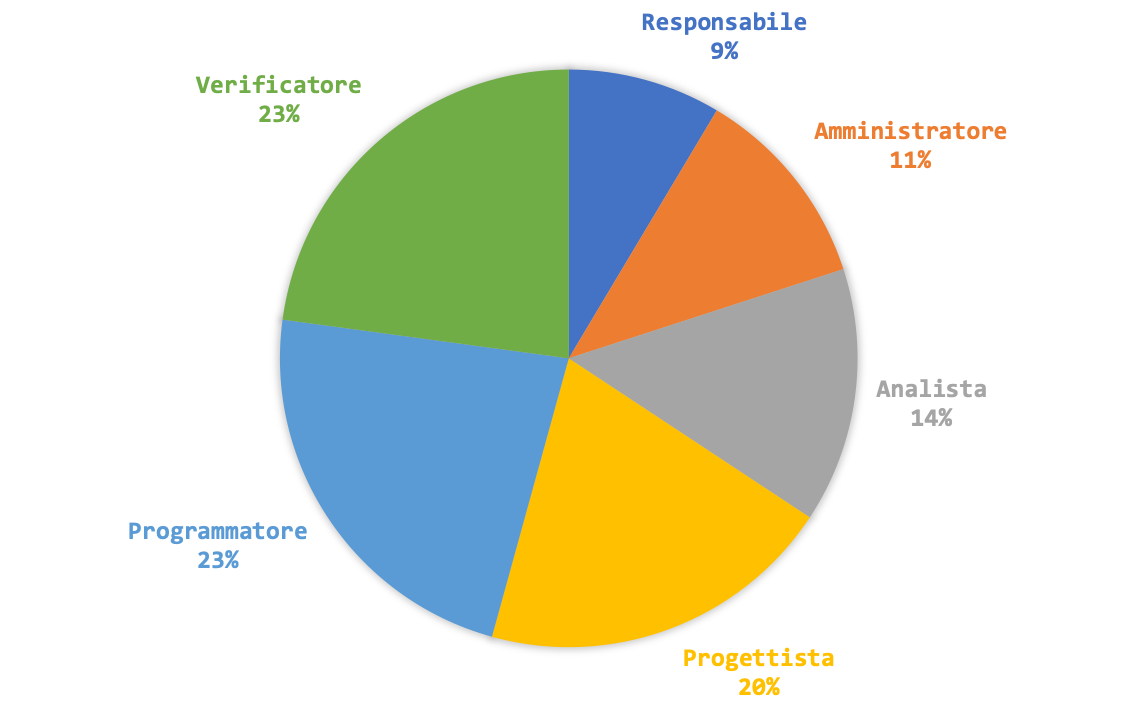
\includegraphics[width=0.8\linewidth]{images/consuntivo/ConsIncr1-2.png}
				\caption{Diagramma percentuale ore/ruolo nell'incremento I}
				\label{fig:consuntivo diagramma costi ruolo incremento I}
			\end{figure}

		\paragraph{Conclusioni}
			Durante l'incremento I il gruppo ha lavorato mantenendo il numero di ore che erano state preventivate. È stato necessario però svolgere alcuni cambiamenti nella suddivisione oraria per ruolo, in particolare:
			\begin{itemize}
				\item \textbf{amministratore:} la configurazione degli strumenti da parte dell'amministratore ha richiesto meno tempo di ciò che era stato preventivato.
				\item \textbf{progettista:} grazie all'analisi approfondita svolta nelle fase precedenti per quanto riguarda l'architettura del sistema, il ruolo del progettista ha richiesto un'ora in meno di ciò che era stato preventivato.
				\item \textbf{verificatore:} si è deciso di assegnare il surplus di due ore al verificatore per garantire una qualità superiore del prodotto al committente e al proponente.
			\end{itemize}
			Alla luce dei cambiamenti effettuati il risultato è che il gruppo ha risparmiato in totale € 27,00 investendo le stesse ore preventivate.
			\pagebreak
		
		\paragraph{Preventivo a finire}
			L'inizio dello sviluppo sta procedendo in modo positivo, specialmente nel primo periodo di progettazione dell'incremento, che ha richiesto meno risorse di quanto preventivato, segno di una progettazione troppo prudente.
			\newline
			È stato scelto di impiegare le risorse rimaste disponibili per potenziare la verifica in modo da garantire una maggiore qualità nel primo incremento che costituisce la base del prodotto.
			\newline
			Di conseguenza, anche a seguito dei lievi cambiamenti riportati, è stato deciso di non modificare il preventivo in quanto si è ritenuto che la pianificazione svolta garantisca il raggiungimento degli obiettivi preposti nei tempi stabiliti.	

		\subsubsection{Incremento II }
		Le ore di lavoro svolte in questo periodo sono volte alla creazione della struttura base del \glock{gateway} ed alla decisione della struttura JSON dei dati da inviare a Kafka. Verrà inoltre implementato un primo protocollo di comunicazione.
		\paragraph{Prospetto orario}
			Nella tabella in seguito viene illustrato il cambiamento nel numero d'ore di ogni persona, per ogni ruolo ricoperto:
			
			\rowcolors{2}{lightest-grayest}{white}
			\begin{longtable}{|l|c|c|c|c|c|c|c|}
				\hline
				\rowcolor{lighter-grayer}
				\textbf{Nome} & \textbf{Re} & \textbf{Am} & \textbf{An} & \textbf{Pg}  & \textbf{Pr}   & \textbf{Ve} & \textbf{Totale} \\
				\hline
				\endfirsthead
				\hline
				Giuseppe Vito Bitetti  & 1 & 0 & 0 & 3 & 1 (+1) & 1 (-1) & 6\\
				\hline
				\hline
				Lorenzo Dei Negri      & 0 & 0 & 0 & 0 & 3 & 3 & 6 \\
				\hline
				\hline
				Nicolò Frison 			  & 3 & 0 & 0 & 0 & 3 & 0 & 6 \\
				\hline
				\hline
				Fouad Mouad 			& 0 & 3 & 2 (-1) & 1 (+1) & 0 & 0 & 6 \\
				\hline
				\hline
				Mariano Sciacco			 & 0 & 0 & 0 & 2 & 0 & 4 & 6 \\
				\hline
				\hline
				Alessandro Tommasin & 0 & 1 & 0 & 0 & 5 & 0 & 6 \\
				\hline
				\hline
				Giovanni Vidotto 		& 0 & 2 & 0 & 4 & 0 & 0 & 6\\
				\hline 
				\textbf{Totale} 		   & 4 &  6 & 2 (-1) & 11 (+1) & 12 (+1) & 8 (-1) & 42\\
				\hline 
				
				\caption{Tabella consuntiva contenente il prospetto orario per l'incremento II}
			\end{longtable}
			\pagebreak
			
			La tabella può essere riassunta nel seguente istogramma:
			
			\begin{figure}[H]
				\centering
				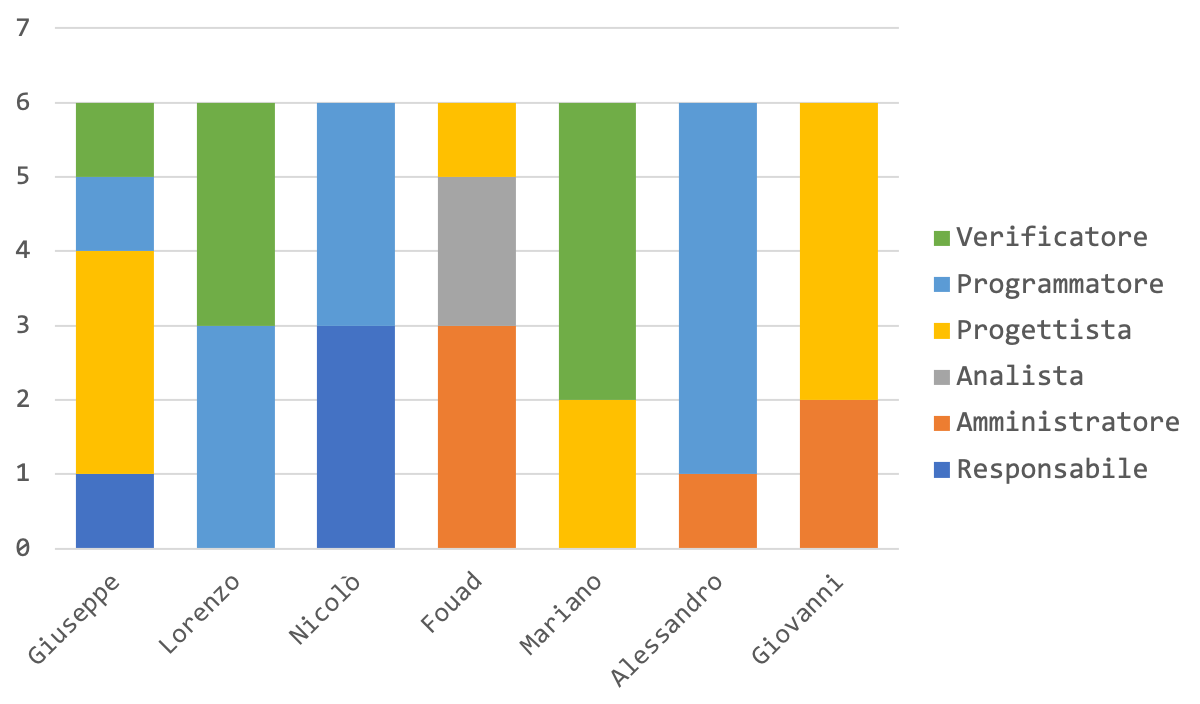
\includegraphics[width=0.8\linewidth]{images/consuntivo/ConsIncr2-1.png}
				\caption{Diagramma consuntivo ore/ruolo componenti dell'incremento II}
				\label{fig:consuntivo diagramma suddivione ruoli incremento II}
			\end{figure}
			
		\paragraph{Prospetto economico}
			In base al prospetto orario, quello economico sarà il seguente: 
			
			\rowcolors{2}{white}{lightest-grayest}
			\begin{longtable}{|l|c|c|c|c|c|c|c|}
				\hline
				\rowcolor{lighter-grayer}
				\textbf{Ruolo} & \textbf{Ore} & \textbf{Costo in €} \\
				\hline
				\endfirsthead
				\hline
			Responsabile 	    & 4 & 120,00\\
			\hline 
			\hline
			Amministratore	  & 6 & 120,00\\
			\hline
			\hline
			Analista 				& 2 (-1) & 50,00 (-25,00) \\
			\hline
			\hline
			Progettista 		  & 10 (+1) & 220,00 (+22,00)\\
			\hline
			\hline
			Programmatore 	 & 12 (+1) & 180,00 (+15,00)\\
			\hline
			\hline
			Verificatore 		  & 8 (-1) & 120,00 (-15,00) \\
			\hline
			\textbf{Totale} 	& 42 & 810,00 (-3,00) \\
			\hline
				
				\caption{Tabella contenente il prospetto economico in riferimento al prospetto orario}
			\end{longtable}
		\pagebreak
			
			La tabella può essere riassunta nel seguente areogramma:
			\begin{figure}[H]
				\centering
				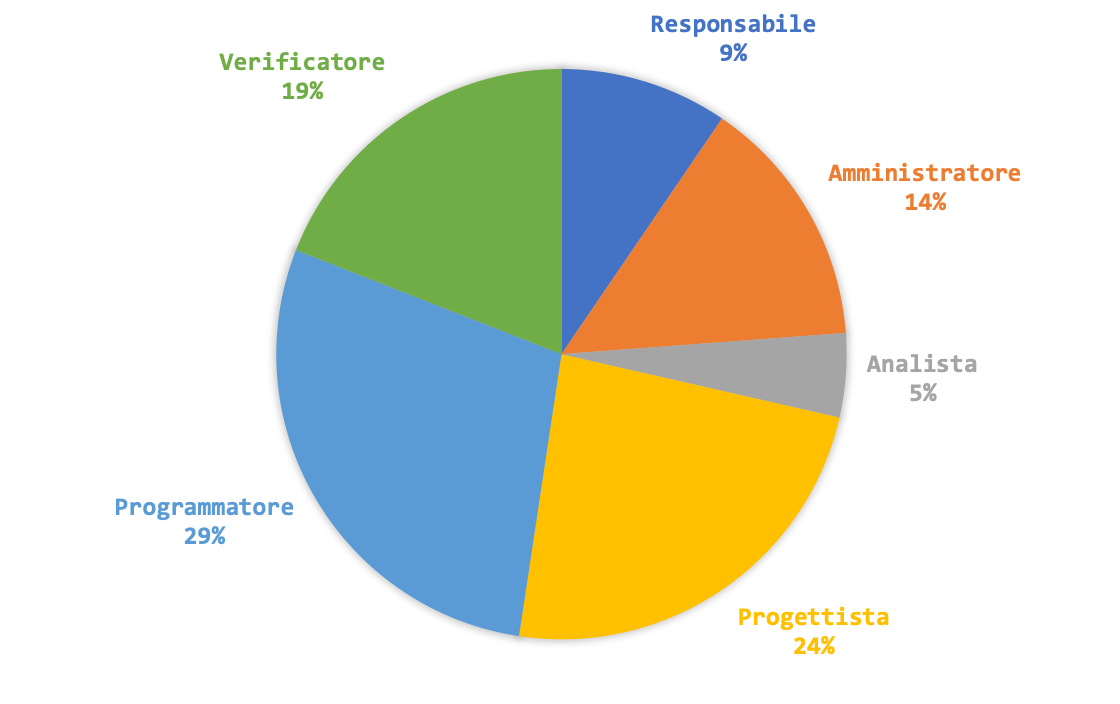
\includegraphics[width=0.8\linewidth]{images/consuntivo/ConsIncr2-2.png}
				\caption{Diagramma percentuale ore/ruolo nell'incremento II}
				\label{fig:consuntivo diagramma costi ruolo incremento II}
			\end{figure}

			\paragraph{Conclusioni}
			Durante l'incremento II il gruppo ha lavorato mantenendo il numero di ore che erano state preventivate. È stato necessario però svolgere alcuni cambiamenti nella suddivisione oraria per ruolo, in particolare:
			\begin{itemize}
				\item \textbf{analista:} la comprensione dei requisiti in riferimento agli incrementi da svolgere ha richiesto un'ora in meno del suddetto ruolo;
				\item \textbf{progettista:} la progettazione del protocollo di comunicazione ha richiesto un'ora in più del ruolo di progettista per idearne la struttura base indispensabile alla comunicazione;
				\item \textbf{programmatore:} la complessità del gateway e l'uso del framework utilizzato ha fatto si che fosse necessaria un'ora in più del ruolo di programmatore;
				\item \textbf{verificatore:} il lavoro in più che è stato necessario per il progettista ha reso più veloce il processo di verifica ed ha portato quindi a risparmiare un'ora del ruolo di verificatore.
			\end{itemize}
			Alla luce dei cambiamenti effettuati il risultato è che il gruppo ha risparmiato in totale € 30,00 investendo le stesse ore preventivate.
			\pagebreak
		
		\paragraph{Preventivo a finire}
			Lo sviluppo sta procedendo in modo positivo, nonostante alcune difficoltà riscontrate nell'utilizzo di nuove tecnologie e strumenti necessari per la realizzazione dell'incremento pianificato.
			\newline
			Tuttavia, avendo potuto intensificare la verifica nello scorso incremento, si è ritenuto ragionevole sopportare la sua riduzione in questa fase. In questo modo è stato possibile non intervenire attivamente sul preventivo, potendo, quindi, dedicare più tempo allo studio delle nuove tecnologie utilizzate.

%%%%%%%%%%%%%%%%%%%%%%%%%%%%%%%%%%%%%%%%%%%%%%%%%%%%%%%%%%%%%%%%%%%%%%%%%%%%%%%%%%%%%%%%%%%%%%%%%%%%%%%%%%%%%%%%%%
		
		\subsubsection{Incremento III }
		Le ore di lavoro svolte in questo periodo sono volte alla progettazione dell'interfaccia delle \glock{API} ed all'implementazione delle operazioni di lettura dei dati tramite le \glock{API}.
		\paragraph{Prospetto orario}
			Nella tabella in seguito viene illustrato il cambiamento nel numero d'ore di ogni persona, per ogni ruolo ricoperto:
			
			\rowcolors{2}{lightest-grayest}{white}
			\begin{longtable}{|l|c|c|c|c|c|c|c|}
				\hline
				\rowcolor{lighter-grayer}
				\textbf{Nome} & \textbf{Re} & \textbf{Am} & \textbf{An} & \textbf{Pg}  & \textbf{Pr}   & \textbf{Ve} & \textbf{Totale} \\
				\hline
				\endfirsthead
				\hline
				Giuseppe Vito Bitetti & 0 & 0 & 0 & 1 (+1) & 2 (-1) & 3 & 6\\
				\hline
				\hline
				Lorenzo Dei Negri & 0 & 0 & 0 & 3 & 0 & 3 & 6\\
				\hline
				\hline
				Nicolò Frison & 3 & 0 & 0 & 2 & 0 & 1 & 6 \\
				\hline
				\hline
				Fouad Mouad & 0 & 0 & 0 & 3 & 3 & 0 & 6\\
				\hline
				\hline
				Mariano Sciacco & 0 & 3 & 0 & 0 & 3 & 0 & 6 \\
				\hline
				\hline
				Alessandro Tommasin & 0 & 0 & 0 & 2 & 2 & 0 & 6\\
				\hline
				\hline
				Giovanni Vidotto & 0 & 0 & 0 & 3 (+1) & 0 & 3 (-1) & 6 \\
				\hline 
				\textbf{Totale} & 3 &  3 & 0 & 14 (+2) & 10 (-1) & 12 (-1) & 42 \\
				\hline 
				
				\caption{Tabella consuntiva contenente il prospetto orario per l'incremento III}
			\end{longtable}
			\pagebreak
			
			La tabella può essere riassunta nel seguente istogramma:
			
			\begin{figure}[H]
				\centering
				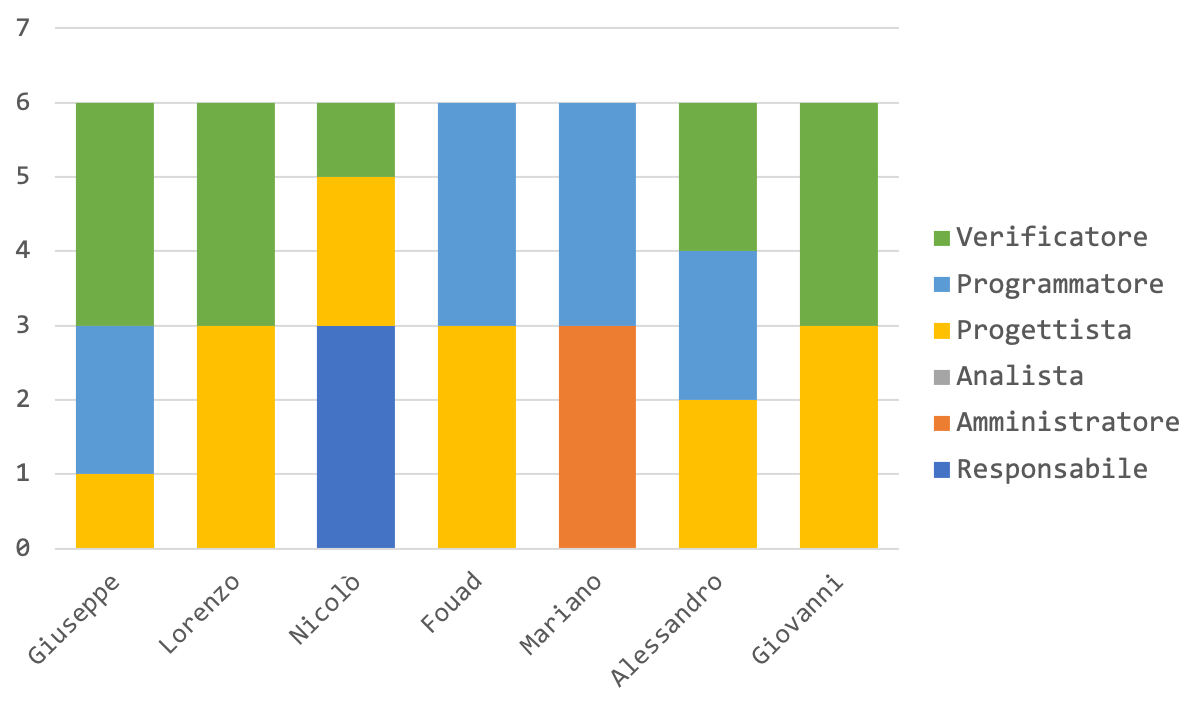
\includegraphics[width=0.8\linewidth]{images/consuntivo/ConsIncr3-1.png}
				\caption{Diagramma consuntivo ore/ruolo componenti dell'incremento III}
				\label{fig:consuntivo diagramma suddivione ruoli incremento III}
			\end{figure}
			
		\paragraph{Prospetto economico}
			In base al prospetto orario, quello economico sarà il seguente: 
			
			\rowcolors{2}{white}{lightest-grayest}
			\begin{longtable}{|l|c|c|c|c|c|c|c|}
				\hline
				\rowcolor{lighter-grayer}
				\textbf{Ruolo} & \textbf{Ore} & \textbf{Costo in €} \\
				\hline
				\endfirsthead
				\hline
				Responsabile 	    & 3 & 90,00 \\
				\hline 
				\hline
				Amministratore	  & 3 & 60,00\\
				\hline
				\hline
				Analista 				& - & -\\
				\hline
				\hline
				Progettista 		  & 14 (+2) & 308,00 (+44,00)\\
				\hline
				\hline
				Programmatore 	 & 10 (-1) & 150,00 (-15,00) \\
				\hline
				\hline
				Verificatore 		  & 12 (-1) & 180,00 (-15,00)\\
				\hline
				\textbf{Totale} 	& 42 & 788,00 (+14,00)\\
				\hline 
					
				\caption{Tabella contenente il prospetto economico in riferimento al prospetto orario}
			\end{longtable}
		\pagebreak
			
			La tabella può essere riassunta nel seguente areogramma:
			\begin{figure}[H]
				\centering
				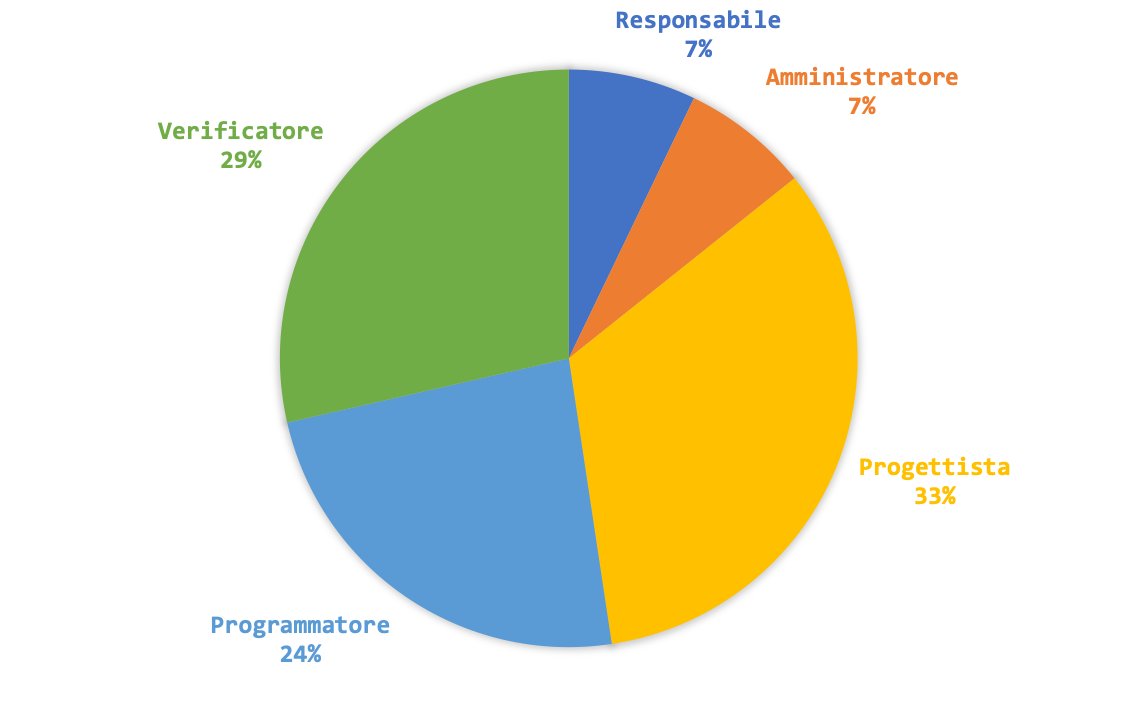
\includegraphics[width=0.8\linewidth]{images/consuntivo/ConsIncr3-2.png}
				\caption{Diagramma percentuale ore/ruolo nell'incremento III}
				\label{fig:consuntivo diagramma costi ruolo incremento III}
			\end{figure}

		\paragraph{Conclusioni}
			Durante l'incremento III il gruppo ha lavorato mantenendo il numero di ore che erano state preventivate. È stato necessario però svolgere alcuni cambiamenti nella suddivisione oraria per ruolo, in particolare:
			\begin{itemize}
				\item \textbf{progettista:} la progettazione delle API ha richiesto due ore in più del ruolo di progettista per creare la struttura base delle API stesse;
				\item \textbf{programmatore:} la qualità del lavoro svolto in fase di progettazione ha fatto si che fosse necessaria un'ora in meno del ruolo di programmatore per implementare l'incremento pianificato;
				\item \textbf{verificatore:} il lavoro in più che è stato necessario per il progettista ha reso più veloce il processo di verifica ed ha portato quindi a risparmiare un'ora del ruolo di verificatore.
			\end{itemize}
			Alla luce dei cambiamenti effettuati il risultato è che il gruppo ha risparmiato in totale € 16,00 investendo le stesse ore preventivate.
		
		\paragraph{Preventivo a finire}
			Lo sviluppo procede in modo positivo, nonostante alcune difficoltà riscontrate nella progettazione di dettaglio dell'incremento pianificato. Tuttavia, l'intensificazione della progettazione ha favorito la codifica di quanto progettato, permettendo un risparmio di tempo da parte del programmatore.
			\newline
			D'altro canto, questo ha anche comportato la riduzione di un'ora del tempo previsto per la verifica, ma, sebbene sia il secondo incremento consecutivo che risente di questo indebolimento della verifica, si ritiene che ciò possa essere recuperato negli incrementi successivi.
			\newline
			Di conseguenza non è stato ritenuto necessario modificare il preventivo definito in \S5.
				
		%%%%%%%%%%%%%%%%%%%%%%%%%%%%%%%%%%%%%%%%%%%%%%%%%%%%%%%%%%%%%%%%%%%%%%%%%%%%%%%%%%%%%%%%%%%%%%%%%%%%%%%%%%%%%%%%%%
		
		\subsubsection{Incremento IV}
		Le ore di lavoro svolte in questo periodo sono volte alla configurazione di base della web app e reperimento dati dalle \glock{API}.
		\paragraph{Prospetto orario}
			Nella tabella in seguito viene illustrato il cambiamento nel numero d'ore di ogni persona, per ogni ruolo ricoperto:
			
			\rowcolors{2}{lightest-grayest}{white}
			\begin{longtable}{|l|c|c|c|c|c|c|c|}
				\hline
				\rowcolor{lighter-grayer}
				\textbf{Nome} & \textbf{Re} & \textbf{Am} & \textbf{An} & \textbf{Pg}  & \textbf{Pr}   & \textbf{Ve} & \textbf{Totale} \\
				\hline
				\endfirsthead
				\hline
				Giuseppe Vito Bitetti & 2 & 0 & 0 & 0 & 4 & 0 & 6\\
				\hline
				\hline
				Lorenzo Dei Negri & 2 & 0 & 0 & 1 (-1) & 0 & 3 (+1) & 6\\
				\hline
				\hline
				Nicolò Frison & 0 & 0 & 0 & 1 (-1) & 4 & 1 (+1) & 6\\
				\hline
				\hline
				Fouad Mouad & 0 & 3 & 0 & 0 & 0 & 3 & 6\\
				\hline
				\hline
				Mariano Sciacco & 3 & 0 & 0 & 0 & 3 & 0 & 6\\
				\hline
				\hline
				Alessandro Tommasin & 0 & 0 & 2 & 0 & 0 & 4 & 6\\
				\hline
				\hline
				Giovanni Vidotto & 0 & 0 & 0 & 5 & 0 & 1 & 6\\
				\hline 
				\textbf{Totale} & 7 &  3 & 4 & 7 (-2) & 11  & 12 (+2) & 42 \\
				\hline 
				
				\caption{Tabella consuntiva contenente il prospetto orario per l'incremento IV}
			\end{longtable}
			
			La tabella può essere riassunta nel seguente istogramma:
			
			\begin{figure}[H]
				\centering
				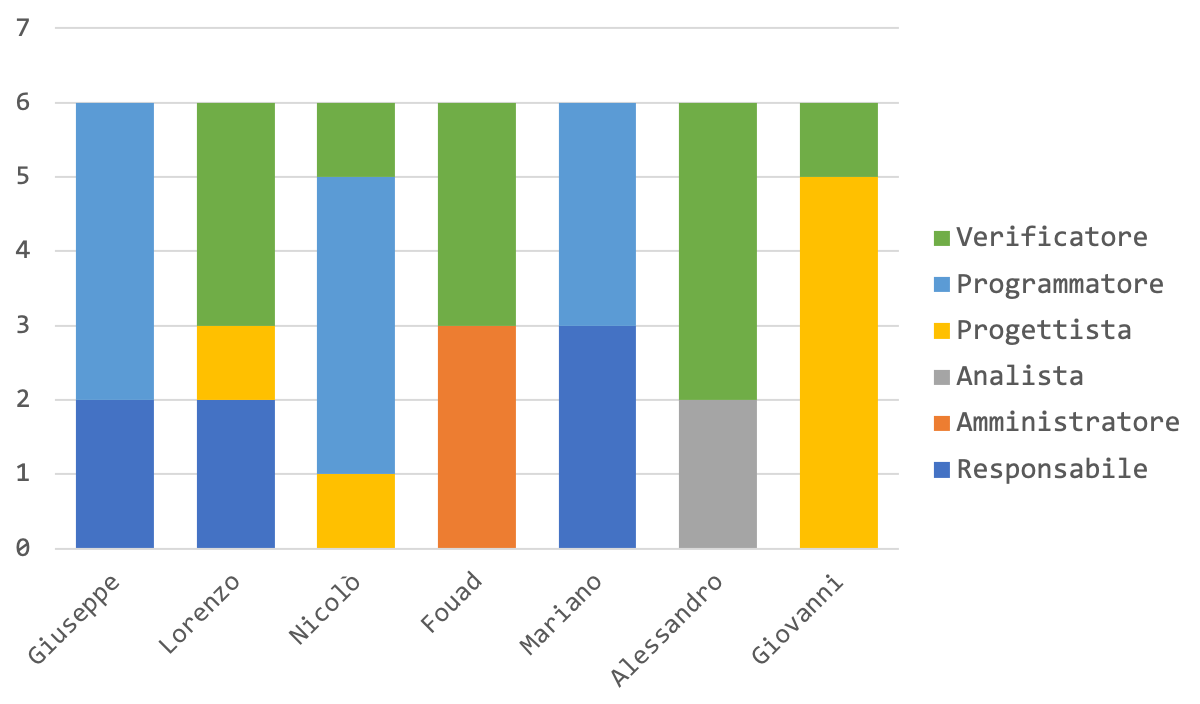
\includegraphics[width=0.8\linewidth]{images/consuntivo/ConsIncr4-1.png}
				\caption{Diagramma consuntivo ore/ruolo componenti dell'incremento IV}
				\label{fig:consuntivo diagramma suddivisione ruoli incremento IV}
			\end{figure}
			
		\paragraph{Prospetto economico}
			In base al prospetto orario, quello economico sarà il seguente: 
			
			\rowcolors{2}{white}{lightest-grayest}
			\begin{longtable}{|l|c|c|c|c|c|c|c|}
				\hline
				\rowcolor{lighter-grayer}
				\textbf{Ruolo} & \textbf{Ore} & \textbf{Costo in €} \\
				\hline
				\endfirsthead
				\hline
				Responsabile 	    & 7 & 210,00\\
				\hline 
				\hline
				Amministratore	  & 3 & 60,00\\
				\hline
				\hline
				Analista 				& 2 & 50,00\\
				\hline
				\hline
				Progettista 		  & 7 (-2) & 154,00 (-44,00)\\
				\hline
				\hline
				Programmatore 	 & 11 & 165,00\\
				\hline
				\hline
				Verificatore 		  & 10 (+2) & 180,00 (+30,00) \\
				\hline
				\textbf{Totale} 	& 42 & 819,00 (-14,00)\\
				\hline
				
				\caption{Tabella contenente il prospetto economico in riferimento al prospetto orario}
			\end{longtable}
			
			La tabella può essere riassunta nel seguente areogramma:
			\begin{figure}[H]
				\centering
				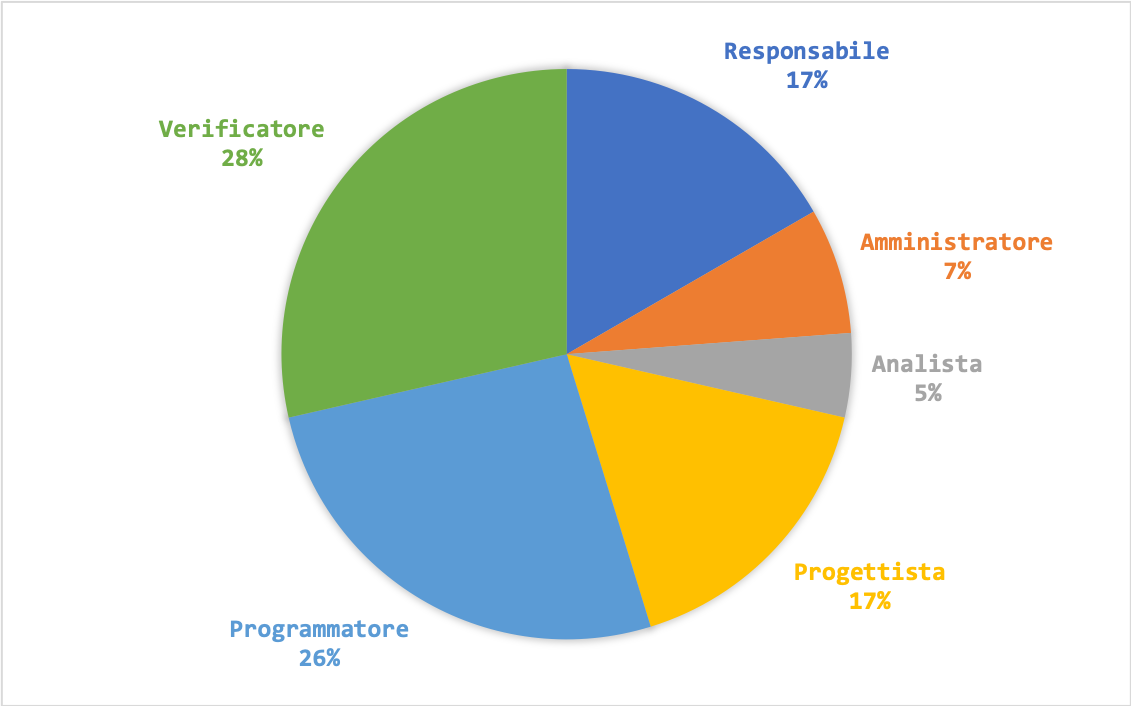
\includegraphics[width=0.8\linewidth]{images/consuntivo/ConsIncr4-2.png}
				\caption{Diagramma percentuale ore/ruolo nell'incremento IV}
				\label{fig:consuntivo diagramma costi ruolo incremento IV}
			\end{figure}
		
		\paragraph{Conclusioni}
			Durante l'incremento IV il gruppo ha lavorato mantenendo il numero di ore che erano state preventivate.
			È stato necessario però svolgere alcuni cambiamenti nella suddivisione oraria per ruolo, in particolare:
			\begin{itemize}
				\item \textbf{progettista:} la progettazione della porzione di web app necessaria all'incremento ha richiesto due ore in meno del ruolo di progettista, grazie all'esperienza maturata precedentemente da parte del progettista;
				\item \textbf{verificatore:} il risparmio maturato dal progettista ha reso possibile investire due ore in più nel ruolo di verificatore.
			\end{itemize}
			Alla luce dei cambiamenti effettuati il risultato è che il gruppo ha risparmiato in totale € 30,00 investendo le stesse ore preventivate.
		
		\paragraph{Preventivo a finire}
			Lo sviluppo procede bene, grazie all'esperienza pregressa del progettista è stato possibile risparmiare del tempo da investire nella verifica, in modo da pareggiare le ore sacrificate in precedenza, senza risentirne a livello di sviluppo dell'incremento.
			\newline
			Di conseguenza il preventivo rimane in linea con quanto definito in \S5.
		
		\pagebreak
		
		\subsubsection{Fase complessiva}
		
		\paragraph{Riepilogo prospetto orario}
			Durante i primi quattro incrementi la distribuzione oraria consuntiva dei ruoli di ogni componente del gruppo può essere riassunta nella seguente tabella:
			
			\rowcolors{2}{lightest-grayest}{white}
			\begin{longtable}{|l|c|c|c|c|c|c|c|}
				\hline
				\rowcolor{lighter-grayer}
				\textbf{Nome} & \textbf{Re} & \textbf{Am} & \textbf{An} & \textbf{Pg}  & \textbf{Pr}   & \textbf{Ve} & \textbf{Totale} \\
				\hline
				\endfirsthead
				
				\hline
				Giuseppe Vito Bitetti 		 & 3 & 0 & 3 & 4 (+1) & 9 & 4 (-1) & 23\\
				\hline
				\hline
				Lorenzo Dei Negri			 & 2 & 0 & 0 & 5 (-2) & 3 & 13 (+2) & 23\\
				\hline
				\hline
				Nicolò Frison				    & 6 & 2 (-1) & 0 & 3 (-1) & 7 & 5 (+2) & 23\\
				\hline
				\hline
				Fouad Mouad 				 & 3 & 6 & 4 (-1) & 4 (+1) & 3 & 3 & 23\\
				\hline
				\hline
				Mariano Sciacco 			 & 3 & 3 & 0 & 5 & 8 & 4 & 23\\
				\hline
				\hline
				Alessandro Tommasin     & 0 & 3 & 2 & 5 & 7 & 6 & 23\\
				\hline
				\hline
				Giovanni Vidotto 			 & 0 & 2 & 0 & 12(+1) & 4 & 5 (-1) & 23\\
				\hline 
				\textbf{Totale}			 		& 17 & 16 (-1) & 9 (-1) & 38 & 41 & 40 (+2) & 161\\
				\hline
				\caption{Tabella contenente il prospetto orario consuntivo per i primi quattro incrementi}
			\end{longtable}
			
			La tabella può essere riassunta nel seguente istogramma:
			\begin{figure}[H]
				\centering
				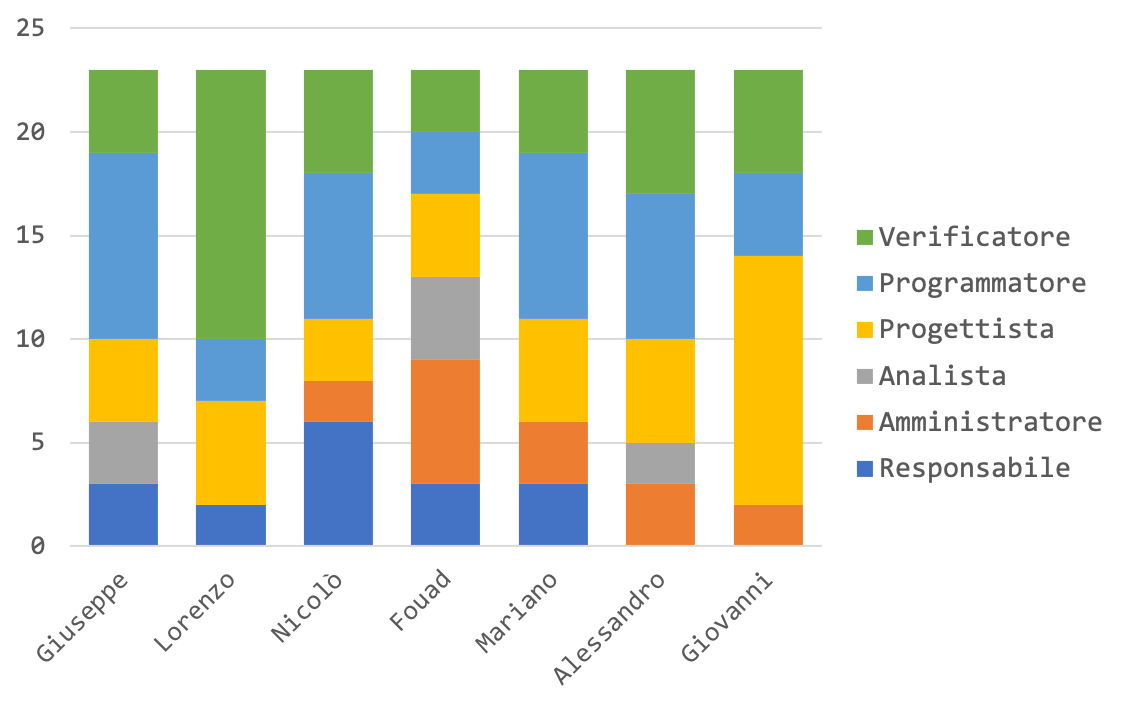
\includegraphics[width=0.8\linewidth]{./images/consuntivo/ConsIncr1-4-1.png}
				\caption{Diagramma ore/ruolo componenti nei primi quattro incrementi}
				\label{fig:diagramma suddivione ruoli incrementi I-IV}
			\end{figure}
			\pagebreak
			
			\paragraph{Riepilogo prospetto economico}
			In base al prospetto orario, quello economico sarà il seguente: 
			
			\rowcolors{2}{white}{lightest-grayest}
			\begin{longtable}{|l|c|c|}
				\hline
				\rowcolor{lighter-grayer}
				\textbf{Ruolo} & \textbf{Ore} & \textbf{Costo in € } \\
				\hline
				\endfirsthead
				
				\hline
				Responsabile 	    & 17 & 510,00\\
				\hline 
				\hline
				Amministratore	   & 16 (-1) & 320,00 (-20,00)\\
				\hline
				\hline
				Analista 				& 9 (-1)& 225,00 (-25,00)\\
				\hline
				\hline
				Progettista 		   & 38 & 836,00\\
				\hline
				\hline
				Programmatore 	  & 41 & 615,00\\
				\hline
				\hline
				Verificatore 		   & 40 (+2) & 600,00\\
				\hline
				\textbf{Totale} 	 & 161 & 3106,00 (-15)\\
				\hline
				\caption{Tabella contenente il prospetto economico in riferimento al prospetto orario}
			\end{longtable}
			
			La tabella può essere riassunta nel seguente areogramma:
			\begin{figure}[H]
				\centering
				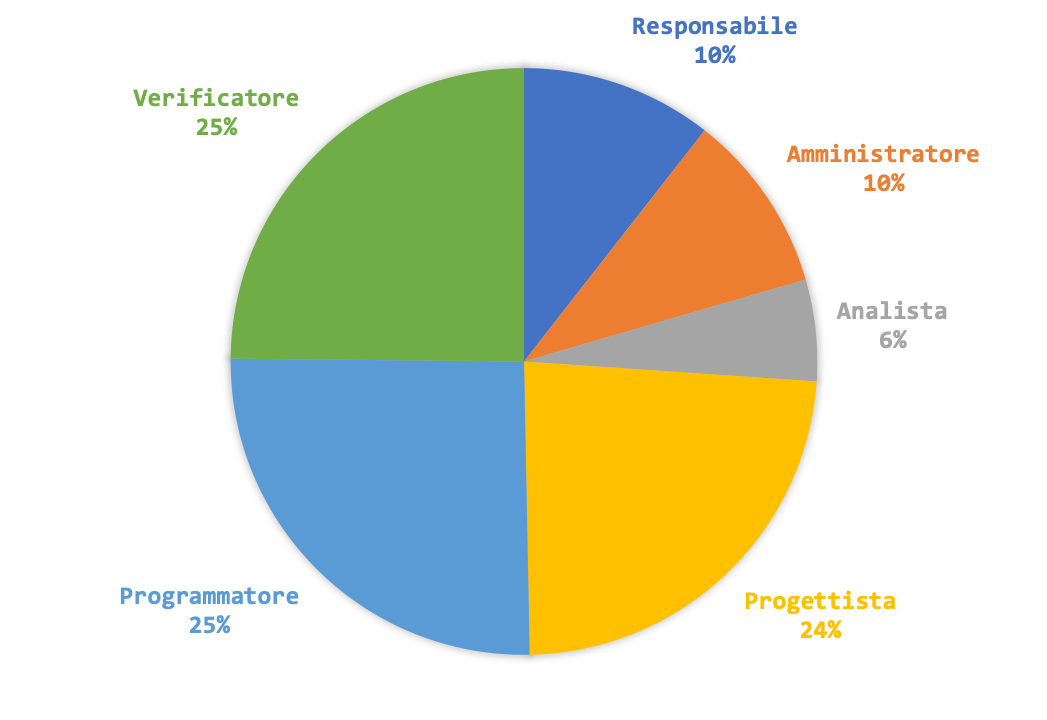
\includegraphics[width=0.8\linewidth]{./images/consuntivo/ConsIncr1-4-2.png}
				\caption{Diagramma consuntivo percentuale ore/ruolo dei primi quattro incrementi}
				\label{fig:diagramma consuntivo costi ruolo incrementi I-IV}
			\end{figure}
		\paragraph{Preventivo a finire}
		In questa prima fase lo sviluppo del prodotto, sebbene leggermente altalenante per quanto riguarda le ore impiegate per i vari ruoli, è stato in linea con quanto preventivato inizialmente; di conseguenza il preventivo a finire resta invariato. 
		\pagebreak
		%%%%%%%%%%%%%%%%%%%%%%%%%%%%%%%%%%%%%%%%%%%%%%%%%%%%%%%%%%%%%%%%%%%%%%%%%%%%%%%%%%%%%%%%%%%%%%%%%%%%%%%%%%%%%%%%%%
		\subsection{Progettazione completa dell'architettura e implementazione delle funzionalità}
		Vedremo in dettaglio i consuntivi dei successivi quattro incrementi, che compongono la fase stessa.  
		\subsubsection{Incremento V }
		Le ore di lavoro del periodo sono volte all'implementazione della configurazione dinamica del gateway.
		\paragraph{Prospetto orario}
			La tabella illustra il cambiamento nel numero d'ore di ogni persona, per ogni ruolo ricoperto:
			
			\rowcolors{2}{lightest-grayest}{white}
			\begin{longtable}{|l|c|c|c|c|c|c|c|}
				\hline
				\rowcolor{lighter-grayer}
				\textbf{Nome} & \textbf{Re} & \textbf{Am} & \textbf{An} & \textbf{Pg}  & \textbf{Pr}   & \textbf{Ve} & \textbf{Totale} \\
				\hline
				\endfirsthead
				\hline
				Giuseppe Vito Bitetti & 0 & 2 & 2 & 0 & 0 & 2 & 6\\
				\hline
				\hline
				Lorenzo Dei Negri & 0 & 0 & 0 & 2 & 4 & 0 & 6\\
				\hline
				\hline
				Nicolò Frison & 2 & 0 & 0 & 0 & 0 & 4 & 6\\
				\hline
				\hline
				Fouad Mouad & 3 (+1) & 0 & 0 & 0 & 3 (-1) & 0 & 6 \\
				\hline
				\hline
				Mariano Sciacco & 0 & 0 & 0 & 3(+2) & 3 & 0(-2) & 6\\
				\hline
				\hline
				Alessandro Tommasin & 0 & 0 & 0 & 3 & 3 & 0 & 6\\
				\hline
				\hline
				Giovanni Vidotto & 0 & 2 & 0 & 0 & 4 & 0 & 6\\
				\hline 
				\textbf{Totale} & 5 (+1) & 4 & 2 & 8 (+2) & 17 (-1) & 6(-2) & 42 \\
				\hline 
				
				\caption{Tabella consuntiva contenente il prospetto orario per l'incremento V}
			\end{longtable}	
			
			La tabella può essere riassunta nel seguente istogramma:
			
			\begin{figure}[H]
				\centering
				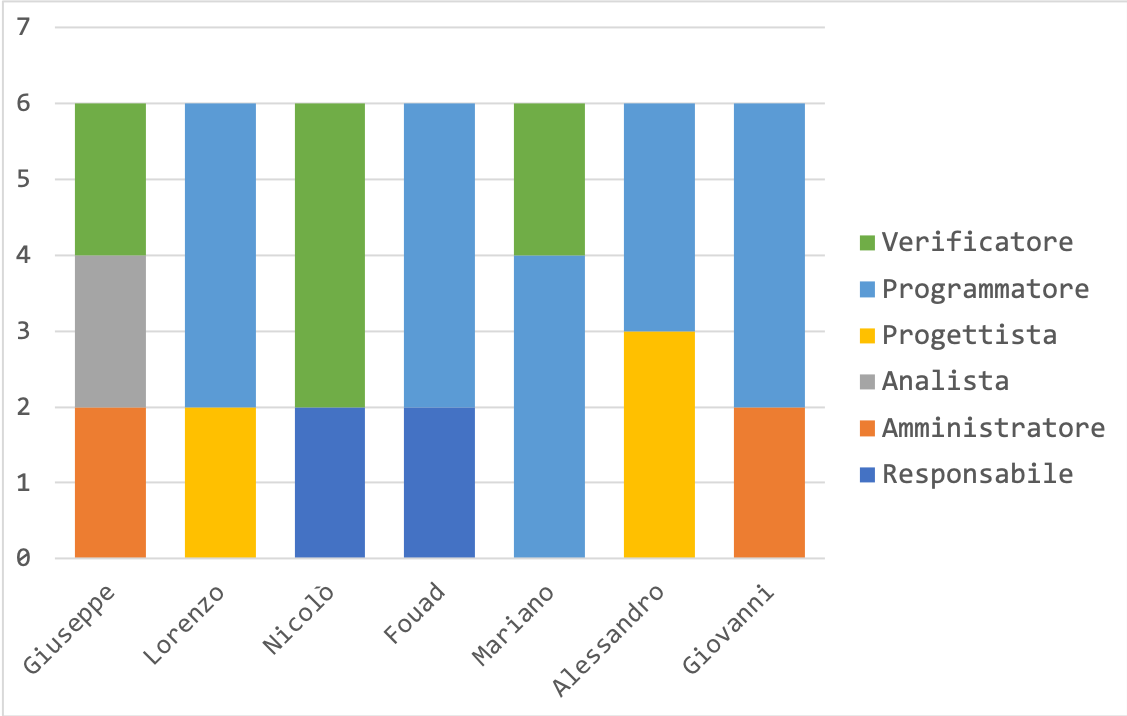
\includegraphics[width=0.75\linewidth]{images/consuntivo/ConsIncr5-1.png}
				\caption{Diagramma consuntivo ore/ruolo componenti dell'incremento V}
				\label{fig:consuntivo diagramma suddivisione ruoli incremento V}
			\end{figure}
			
			
		\paragraph{Prospetto economico}
			In base al prospetto orario, quello economico sarà il seguente: 
			
			\rowcolors{2}{white}{lightest-grayest}
			\begin{longtable}{|l|c|c|c|c|c|c|c|}
				\hline
				\rowcolor{lighter-grayer}
				\textbf{Ruolo} & \textbf{Ore} & \textbf{Costo in €} \\
				\hline
				\endfirsthead
				\hline
				Responsabile 	    & 5 (+1) & 150,00 (+30,00)\\
				\hline 
				\hline
				Amministratore	  & 4 & 80,00\\
				\hline
				\hline
				Analista 				& 2 & 50,00\\
				\hline
				\hline
				Progettista 		  & 8 (+2) & 176,00 (+44,00)\\
				\hline
				\hline
				Programmatore 	 & 17 (-1)  & 255 (-15),00 \\
				\hline
				\hline
				Verificatore 		  & 6 (-2) & 90,00 (-30)\\
				\hline
				\textbf{Totale} 	&  42 & 801,00 (+29,00)\\
				\hline
					
				\caption{Tabella contenente il prospetto economico in riferimento al prospetto orario}
			\end{longtable}
			
			La tabella può essere riassunta nel seguente areogramma:
			\begin{figure}[H]
				\centering
				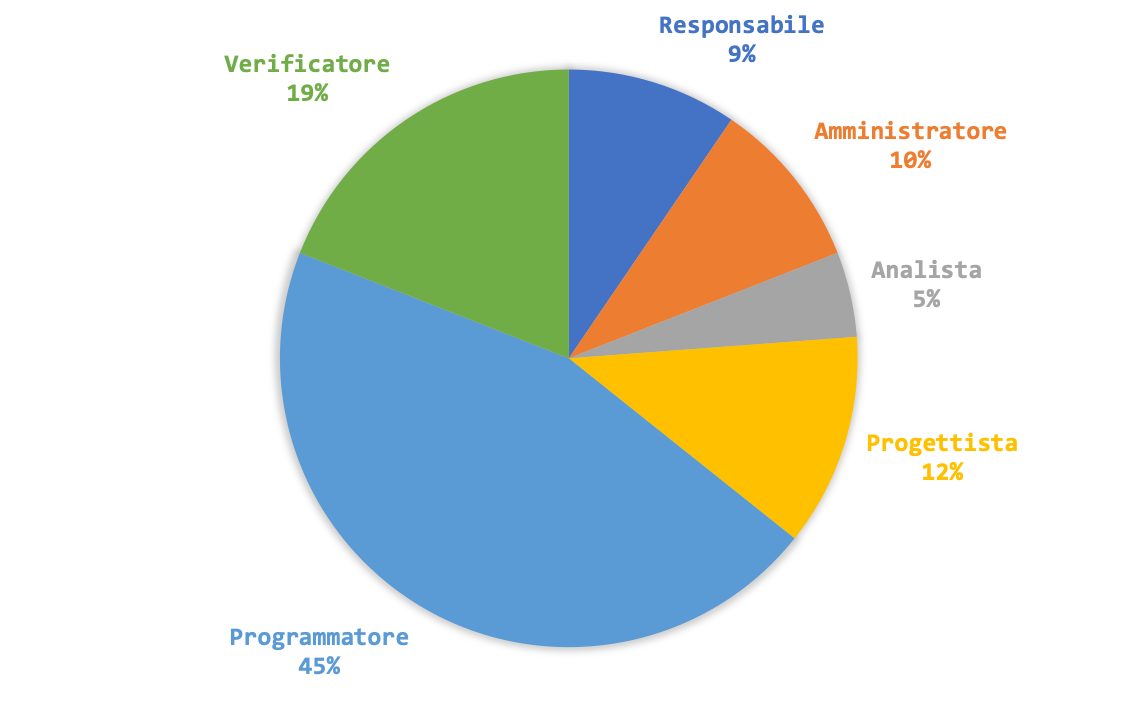
\includegraphics[width=0.8\linewidth]{images/consuntivo/ConsIncr5-2.png}
				\caption{Diagramma percentuale ore/ruolo nell'incremento V}
				\label{fig:consuntivo diagramma costi ruolo incremento V}
			\end{figure}
		\pagebreak
		%Conclusioni per la revisione di progettazione
		\paragraph{Conclusioni}
			Durante l'incremento V il gruppo ha lavorato mantenendo il numero di ore che erano state preventivate. È stato necessario però svolgere alcuni cambiamenti nella suddivisione oraria per ruolo, in particolare:
			\begin{itemize}
				\item \textbf{responsabile:} il ruolo del responsabile è stato svolto più lentamente di ciò che era stato preventivato, richiedendo un'ora in più, a causa dell'onere di approvazione dei documenti per il rilascio esterno che si è rivelato più impegnativo del previsto;
				\item \textbf{progettista:} la progettazione della gestione dinamica della configurazione dei gateway ha richiesto due ore in più del ruolo di progettista, a causa della complessità di aggiornamento della configurazione stessa;
				\item \textbf{programmatore:} la qualità del lavoro svolto in fase di progettazione, unito alla solida base di partenza dello sviluppo del gateway, ha fatto si che fosse necessaria un'ora in meno del ruolo di programmatore per implementare l'incremento pianificato;
				\item \textbf{verificatore:} la qualità del lavoro svolto in fase di codifica, unito alla solida base di partenza del gateway, abbondantemente verificate negli scorsi incrementi, ha fatto si che fossero necessarie due ore in meno del ruolo di programmatore per implementare l'incremento pianificato.
			\end{itemize}
			Alla luce dei cambiamenti effettuati il risultato è che il gruppo ha risparmiato 1,00 € investendo le stesse ore preventivate.
		
		\paragraph{Preventivo a finire}
			Lo sviluppo procede in modo soddisfacente, nonostante le iniziali difficoltà nella progettazione di dettaglio dell'incremento, la qualità del lavoro svolto ha permesso di ridurre le ore di codifica e verifica senza risentirne a livello di sviluppo e qualità dello stesso.
			\newline
			Quindi, nonostante i cambiamenti effettuati al piano orario, l'incremento è stato realizzato secondo la pianificazione preventivata, perciò il preventivo rimane in linea con quanto definito in \S5.
			\pagebreak
			
			
		\subsubsection{Incremento VI }
			Le ore di lavoro svolte in questo periodo sono volte all'implementazione dei  \glock{database} e per la configurazione della comunicazione dei database con \glock{Kafka}.
			\paragraph{Prospetto orario}
			Nella tabella in seguito viene illustrato il cambiamento nel numero d'ore di ogni persona, per ogni ruolo ricoperto:
				\rowcolors{2}{lightest-grayest}{white}
			\begin{longtable}{|l|c|c|c|c|c|c|c|}
				\hline
				\rowcolor{lighter-grayer}
				\textbf{Nome} & \textbf{Re} & \textbf{Am} & \textbf{An} & \textbf{Pg}  & \textbf{Pr}   & \textbf{Ve} & \textbf{Totale} \\
				\hline
				\endfirsthead
				
				\hline
				Giuseppe Vito Bitetti 		 & 0 & 0 & 0 & 2 & 2 & 2 & 6\\
				\hline
				\hline
				Lorenzo Dei Negri			 & 0 & 0 & 0 & 0 & 4 & 2 & 6\\
				\hline
				\hline
				Nicolò Frison				      & 0 & 3 & 0 & 0 & 3 & 0 & 6\\
				\hline
				\hline
				Fouad Mouad 				   & 2 & 0 & 0 & 0 & 2 & 2 & 6\\
				\hline
				\hline
				Mariano Sciacco 			 & 0 & 0 & 0 & 0 & 2 & 4 & 6\\
				\hline
				\hline
				Alessandro Tommasin    & 0 & 0 & 0 & 0 & 2 & 4 & 6\\
				\hline
				\hline
				Giovanni Vidotto 			  & 0 & 0 & 0 & 4 & 2 & 0 & 6\\
				\hline 
				\textbf{Totale}			 		& 2 & 3 & 0 & 6 & 17 & 14 & 42\\
				\hline
				\caption{Tabella consuntiva contenente il prospetto orario per l'incremento VI}
			\end{longtable}	
	
			La tabella può essere riassunta nel seguente istogramma:
			
			\begin{figure}[H]
			\centering
			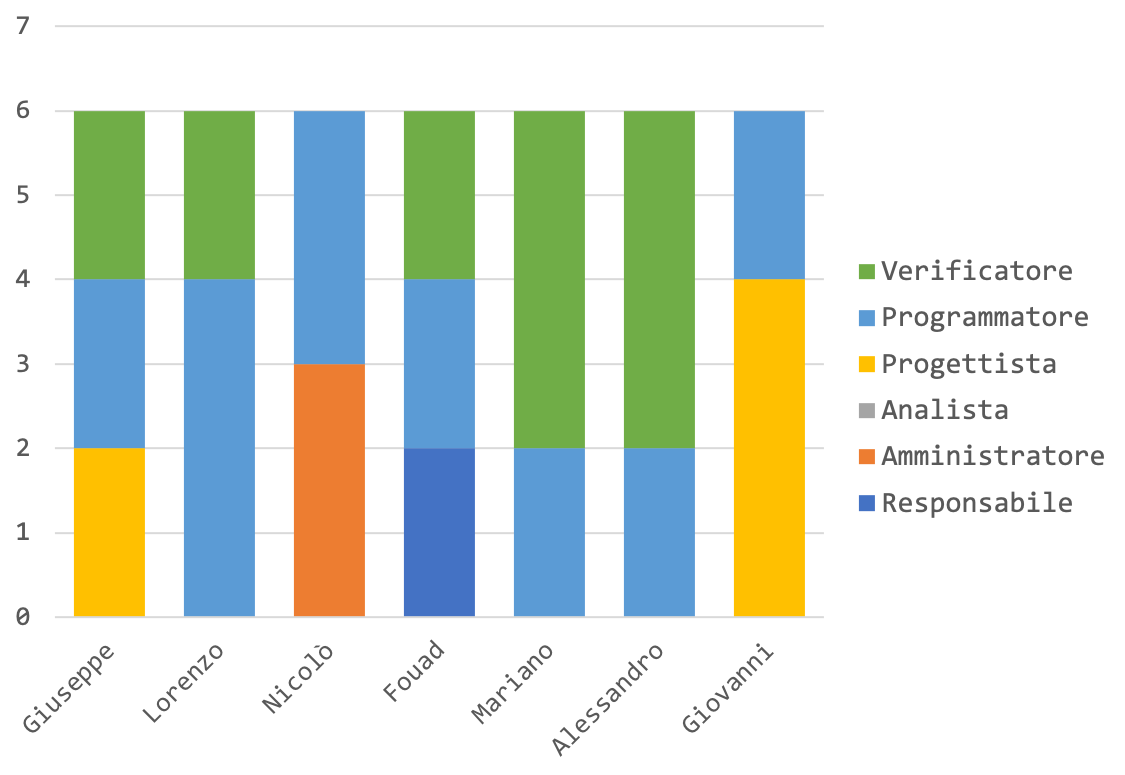
\includegraphics[width=0.75\linewidth]{./images/preventivo/incremento6-1.png}
			\caption{Diagramma consuntivo ore/ruolo componenti dell'incremento VI}
			\label{fig:consuntivo diagramma suddivisione ruoli incremento VI}
			\end{figure}


			\paragraph{Prospetto economico}
			In base al prospetto orario, quello economico sarà il seguente: 
				\rowcolors{2}{white}{lightest-grayest}
			\begin{longtable}{|l|c|c|c|c|c|c|c|}
				\hline
				\rowcolor{lighter-grayer}
				\textbf{Ruolo} & \textbf{Ore} & \textbf{Costo in € } \\
				\hline
				\endfirsthead
				
				\hline
				Responsabile 	    & 3 & 90,00\\
				\hline 
				\hline
				Amministratore	   & 3 & 60,00\\
				\hline
				\hline
				Analista 				& 0 & 0,00\\
				\hline
				\hline
				Progettista 		   & 12 & 264,00\\
				\hline
				\hline
				Programmatore 	  & 11 & 165,00\\
				\hline
				\hline
				Verificatore 		   & 13 & 195,00\\
				\hline
				\textbf{Totale} 	 & 42 & 774,00\\
				\hline
				\caption{Tabella contenente il prospetto economico in riferimento al prospetto orario}
			\end{longtable}
		
				La tabella può essere riassunta nel seguente areogramma:
			\begin{figure}[H]
				\centering
				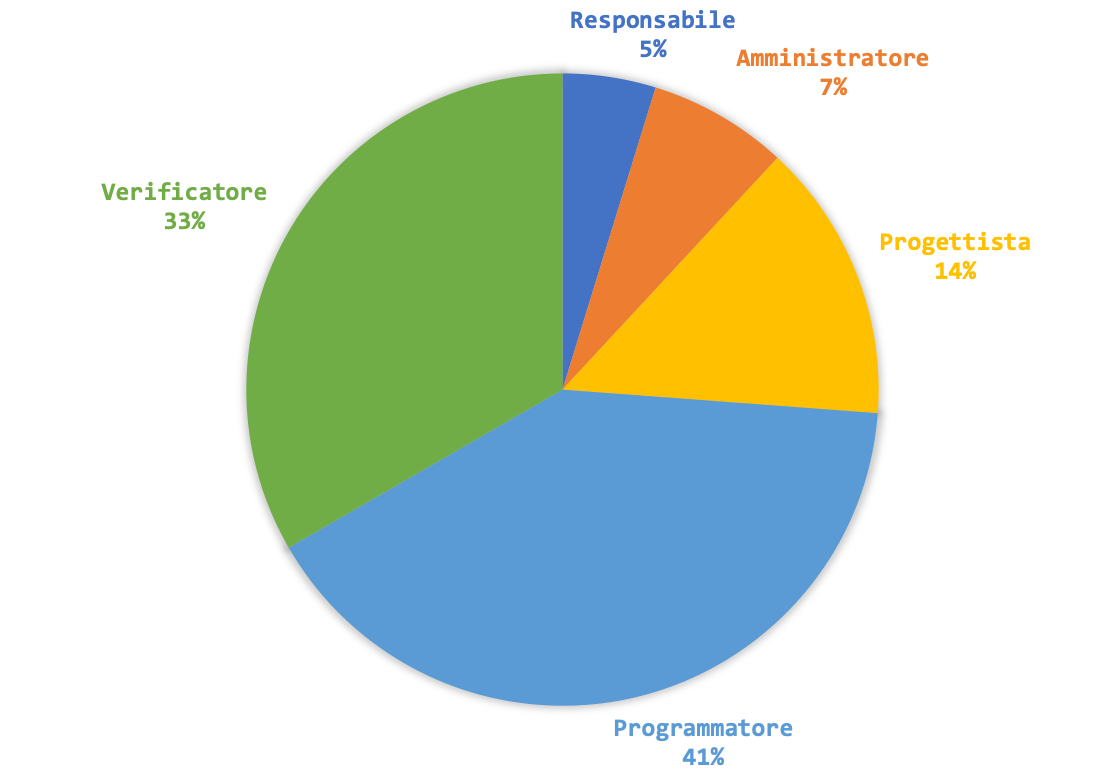
\includegraphics[width=0.8\linewidth]{./images/preventivo/incremento6-2.png}
				\caption{Diagramma percentuale ore/ruolo nell'incremento VI}
				\label{fig:consuntivo diagramma costi ruolo incremento VI}
			\end{figure}
			\pagebreak
			\paragraph{Conclusioni}
				Durante lo sviluppo dell'incremento il gruppo ha lavorato in modo efficiente e professionale, riuscendo a rispettare il numero di ore preventivate, per ogni ruolo coinvolto. 
			
			\paragraph{Preventivo a finire}
				Lo sviluppo dell'incremento è stato molto soddisfacente, infatti l'impegno necessario per completarlo è stato in linea con quanto previsto; di conseguenza il preventivo a finire rimane uguale a quello definito in \S5.
		
		\subsubsection{Incremento VII}
			Le ore di lavoro svolte in questo periodo sono volte all'implementazione base del \glock{bot Telegram}, della schermata di login del sito web e della parte privata e pubblica del sito.
			\paragraph{Prospetto orario}
			Nella tabella in seguito viene illustrato il cambiamento nel numero d'ore di ogni persona, per ogni ruolo ricoperto:
		
			\rowcolors{2}{lightest-grayest}{white}
			\begin{longtable}{|l|c|c|c|c|c|c|c|}
				\hline
				\rowcolor{lighter-grayer}
				\textbf{Nome} & \textbf{Re} & \textbf{Am} & \textbf{An} & \textbf{Pg}  & \textbf{Pr}   & \textbf{Ve} & \textbf{Totale} \\
				\hline
				\endfirsthead
				
				\hline
				Giuseppe Vito Bitetti 		 & 0 & 0 & 0 & 0 & 4 & 2 & 6\\
				\hline
				\hline
				Lorenzo Dei Negri			 & 2 & 0 & 0 & 2 & 0 & 2 & 6\\
				\hline
				\hline
				Nicolò Frison				      & 0 & 0 & 0 & 3 & 0 & 3 & 6\\
				\hline
				\hline
				Fouad Mouad 				   & 0 & 0 & 0 & 2 & 0 & 4 & 6\\
				\hline
				\hline
				Mariano Sciacco 			 & 0 & 0 & 0 & 0 & 6 & 0 & 6\\
				\hline
				\hline
				Alessandro Tommasin    & 0 & 2 & 0 & 2 (-2) & 2 (+2 )& 0 & 6\\
				\hline
				\hline
				Giovanni Vidotto 			  & 0 & 0 & 0 & 1 (+1) & 5 (-1) & 0 & 6\\
				\hline 
				\textbf{Totale}			 		& 2 & 2 & 0 & 10 (-1) & 17 (+1) & 11 & 42\\
				\hline
				\caption{Tabella consuntiva contenente il prospetto orario per il settimo incremento}
			\end{longtable}
		\pagebreak
		La tabella può essere riassunta nel seguente istogramma:
		
		\begin{figure}[H]
			\centering
			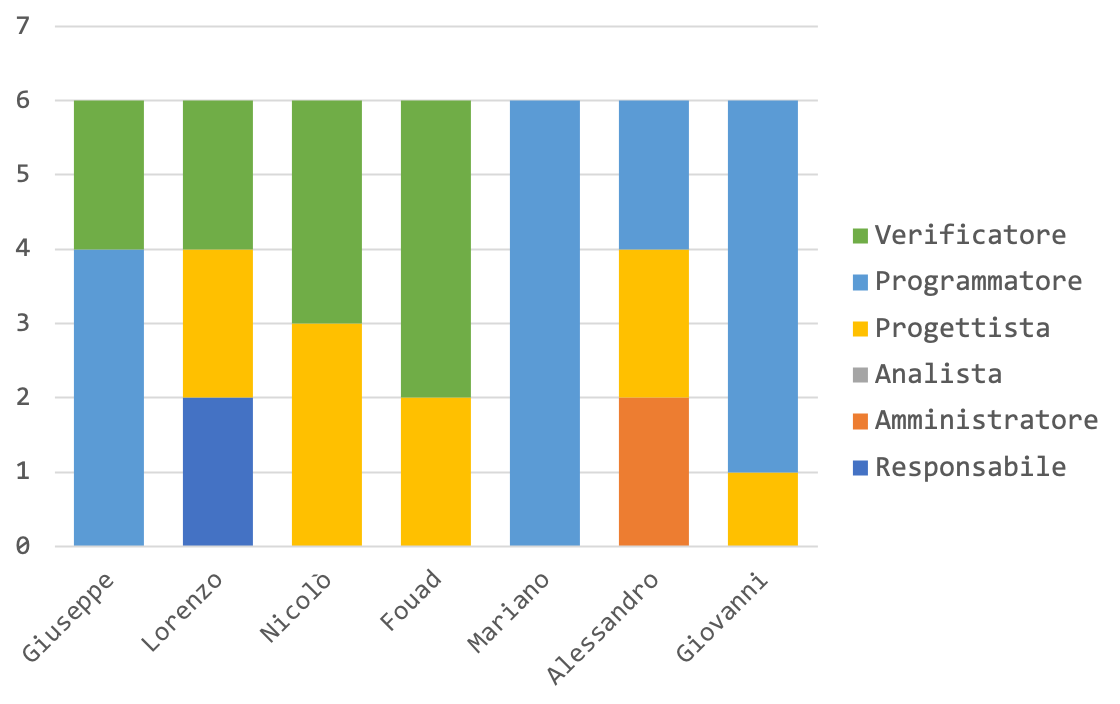
\includegraphics[width=0.8\linewidth]{images/consuntivo/ConsIncr7-1.png}
			\caption{Diagramma consuntivo ore/ruolo componenti dell'incremento VII}
			\label{fig:consuntivo diagramma suddivisione ruoli incremento VII}
		\end{figure}
		
		\paragraph{Prospetto economico}
		In base al prospetto orario, quello economico sarà il seguente: 
		
		\rowcolors{2}{white}{lightest-grayest}
		\begin{longtable}{|l|c|c|}
			\hline
			\rowcolor{lighter-grayer}
			\textbf{Ruolo} & \textbf{Ore} & \textbf{Costo in € } \\
			\hline
			\endfirsthead
			
			\hline
			Responsabile 	    & 2 & 60,00\\
			\hline 
			\hline
			Amministratore	   & 2 & 40,00\\
			\hline
			\hline
			Analista 				 & 0 & 0,00\\
			\hline
			\hline
			Progettista 		   & 10 (-1) & 220,00 (-22,00)\\
			\hline
			\hline
			Programmatore 	  & 17 (+1) & 255,00 (+15,00)\\
			\hline
			\hline
			Verificatore 		   & 11 & 165,00\\
			\hline
			\textbf{Totale} 	 & 42 & 740,00 (-7,00)\\
			\hline
			\caption{Tabella contenente il prospetto economico in riferimento al prospetto orario}
		\end{longtable}
	
		\pagebreak
		
		La tabella può essere riassunta nel seguente areogramma:
		\begin{figure}[H]
			\centering
			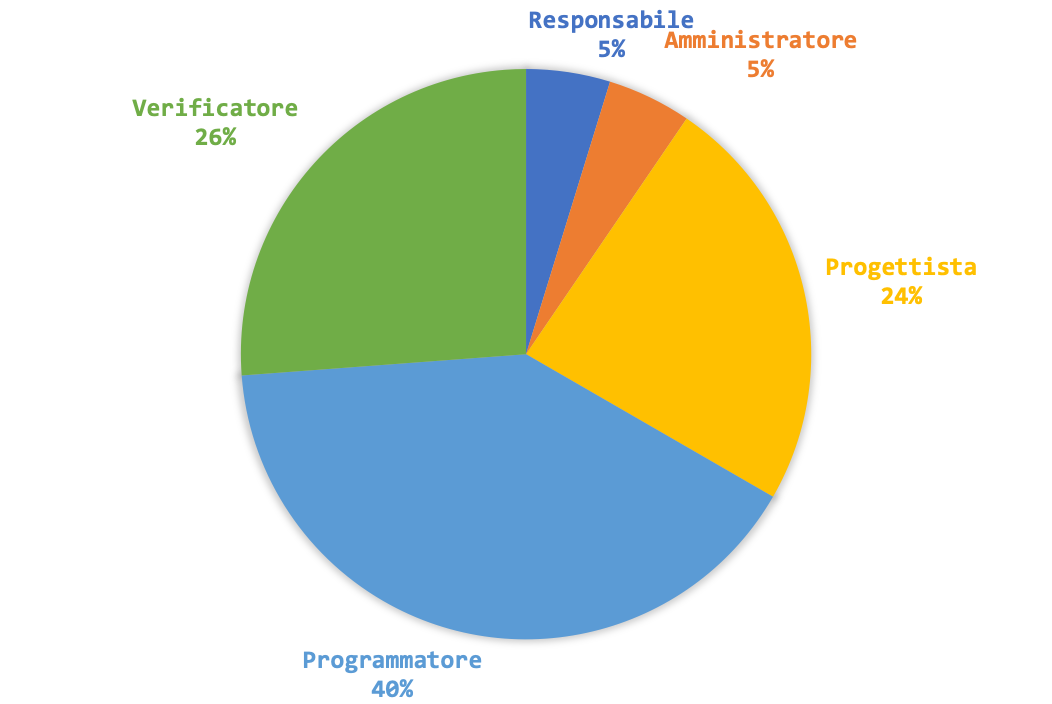
\includegraphics[width=0.8\linewidth]{images/consuntivo/ConsIncr7-2.png}
			\caption{Diagramma percentuale ore/ruolo nell'incremento VII}
			\label{fig:consuntivo diagramma costi ruolo incremento VII}
		\end{figure}
		
		\paragraph{Conclusioni}
			Durante l'incremento VII il gruppo ha lavorato mantenendo il numero di ore che erano state preventivate. È stato necessario però svolgere alcuni cambiamenti nella suddivisione oraria per ruolo, in particolare:
		\begin{itemize}
			\item \textbf{progettista:} la progettazione della porzione di web app necessaria all'incremento ha richiesto un'ora in meno del ruolo di progettista, viste le minori difficoltà riscontrate rispetto a quelle previste;
			\item \textbf{programmatore:} lo sviluppo del bot telegram ha richiesto un'ora in più a causa di alcune difficoltà riscontrate nella fase iniziale.
		\end{itemize}
			Alla luce dei cambiamenti effettuati il risultato è che il gruppo ha risparmiato in totale € 7,00 investendo le stesso numero di ore preventivate.
		
		\paragraph{Preventivo a finire}
			Lo sviluppo procede bene e, nonostante alcune difficoltà iniziali, le tempistiche per l'incremento sono state rispettate, al netto della leggera ridistribuzione oraria citata in precedenza.
			\newline
			È stato necessario impiegare più tempo per lo studio del bot, viste alcune difficoltà iniziali nello sviluppo dello stesso, con il linguaggio Node.JS, dal momento che, la documentazione a riguardo, non è stata di facile comprensione.
			\newline
			Tuttavia, per quanto una problematica riguardante la codifica sia ad alta priorità, e richieda un pronto intervento, la variazione oraria non ha causato un costo supplementare; di conseguenza non si ritiene necessario apportare cambiamenti al preventivo descritto in \S5.
		
		\subsubsection{Incremento VIII}
			Le ore di lavoro svolte in questo periodo sono volte all'implementazione dei grafici per la web app e delle funzioni utili per la generazione dei grafici in tempo reale.
		\paragraph{Prospetto orario}
			Nella tabella in seguito viene illustrato il cambiamento nel numero d'ore di ogni persona, per ogni ruolo ricoperto:
		
		\rowcolors{2}{lightest-grayest}{white}
		\begin{longtable}{|l|c|c|c|c|c|c|c|}
			\hline
			\rowcolor{lighter-grayer}
			\textbf{Nome} & \textbf{Re} & \textbf{Am} & \textbf{An} & \textbf{Pg}  & \textbf{Pr}   & \textbf{Ve} & \textbf{Totale} \\
			\hline
			\endfirsthead
			
			\hline
			Giuseppe Vito Bitetti 		 & 2 & 0 & 0 & 2 & 2 (+2) & 0 (-2) & 6\\
			\hline
			\hline
			Lorenzo Dei Negri			 & 0 & 0 & 0 & 2 & 4 & 0 & 6\\
			\hline
			\hline
			Nicolò Frison				      & 0 & 0 & 0 & 2 & 2 & 2 & 6\\
			\hline
			\hline
			Fouad Mouad 				   & 0 & 0 & 0 & 2 & 2 & 2 & 6\\
			\hline
			\hline
			Mariano Sciacco 			 & 0 & 0 & 0 & 0 (-1) & 1 (+1) & 5 & 6\\
			\hline
			\hline
			Alessandro Tommasin    & 0 & 0 & 0 & 3 & 0 & 3 & 6\\
			\hline
			\hline
			Giovanni Vidotto 			  & 0 & 2 & 0 & 2 & 0 & 2 & 6\\
			\hline 
			\textbf{Totale}			 		 & 2 & 2 & 0 & 13 (-1) & 11 (+3) & 14 (-2) & 42\\
			\hline
			\caption{Tabella consuntiva contenente il prospetto orario per l'ottavo incremento}
		\end{longtable}
		
		La tabella può essere riassunta nel seguente istogramma:
		
		\begin{figure}[H]
			\centering
			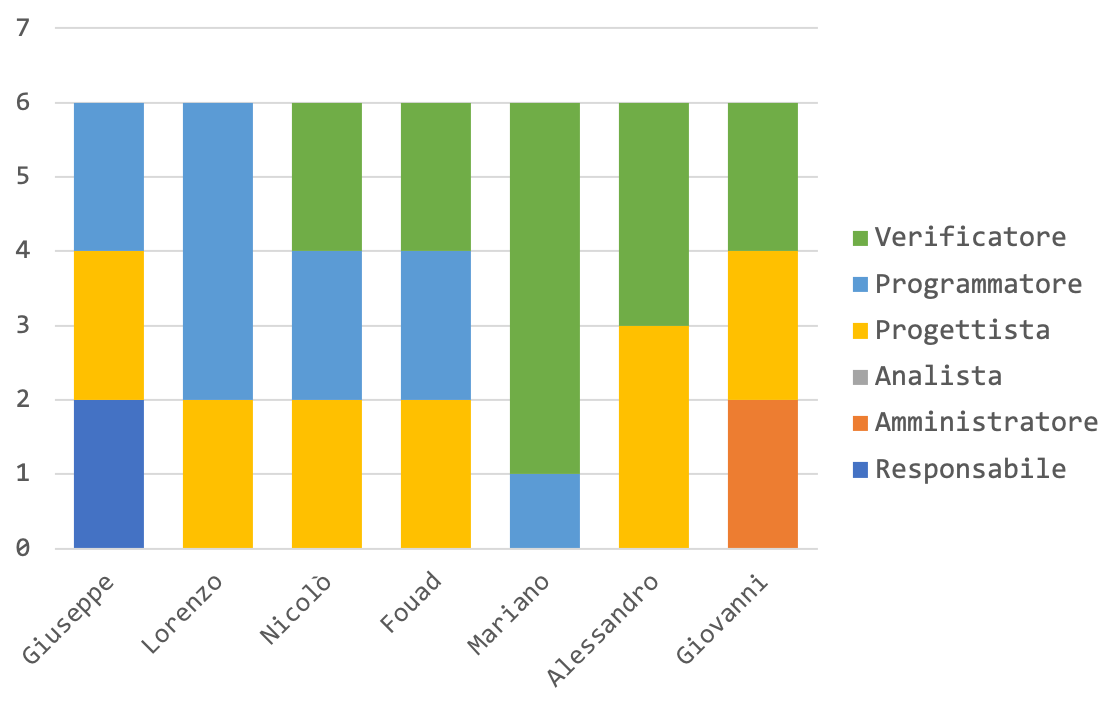
\includegraphics[width=0.8\linewidth]{images/consuntivo/ConsIncr8-1.png}
			\caption{Diagramma consuntivo ore/ruolo componenti dell'incremento VIII}
			\label{fig:consuntivo diagramma suddivisione ruoli incremento VIII}
		\end{figure}
		
		\paragraph{Prospetto economico}
			In base al prospetto orario, quello economico sarà il seguente: 
		
		\rowcolors{2}{white}{lightest-grayest}
		\begin{longtable}{|l|c|c|}
			\hline
			\rowcolor{lighter-grayer}
			\textbf{Ruolo} & \textbf{Ore} & \textbf{Costo in € } \\
			\hline
			\endfirsthead
			
			\hline
			Responsabile 	    & 2 & 60,00\\
			\hline 
			\hline
			Amministratore	   & 2 & 40,00\\
			\hline
			\hline
			Analista 				& - & -\\
			\hline
			\hline
			Progettista 		   & 13 (-1) & 286,00 (-22,00)\\
			\hline
			\hline
			Programmatore 	  & 11 (+3) & 165,00 (+45,00)\\
			\hline
			\hline
			Verificatore 		   & 14 (-2) & 210,00 (-30,00)\\
			\hline
			\textbf{Totale} 	 & 42 & 761,00 (-7,00)\\
			\hline
			\caption{Tabella contenente il prospetto economico in riferimento al prospetto orario}
		\end{longtable}

		
		La tabella può essere riassunta nel seguente areogramma:
		\begin{figure}[H]
			\centering
			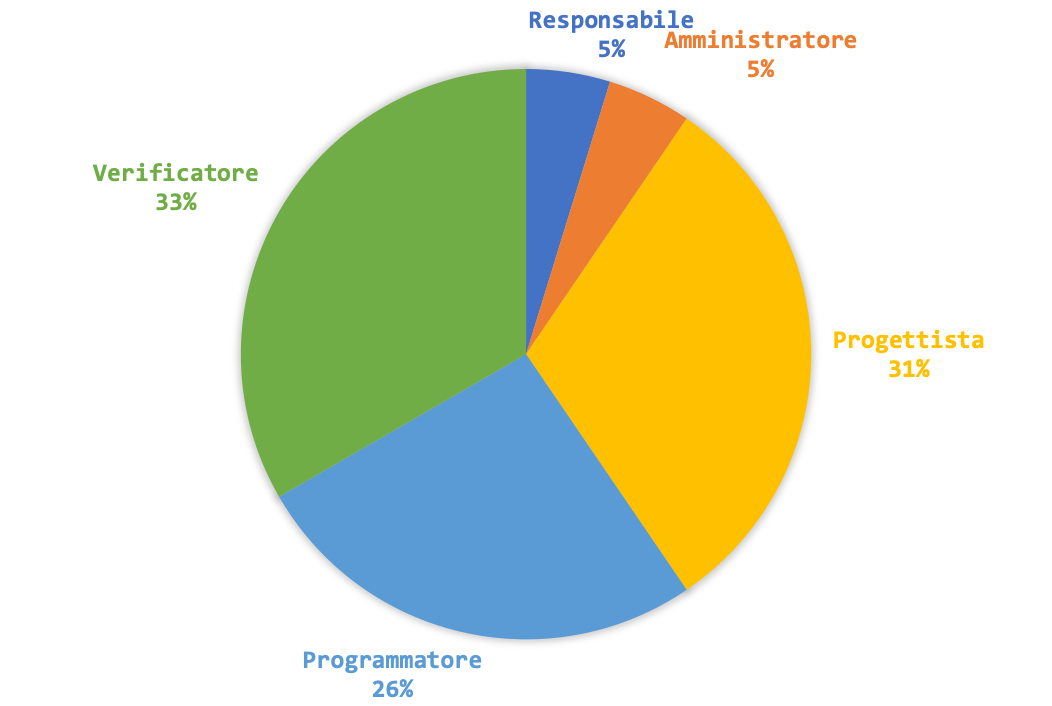
\includegraphics[width=0.8\linewidth]{images/consuntivo/ConsIncr8-2.png}
			\caption{Diagramma percentuale ore/ruolo nell'incremento VIII}
			\label{fig:consuntivo diagramma costi ruolo incremento VIII}
		\end{figure}
		
		\pagebreak
		
		\paragraph{Conclusioni}
			Durante l'incremento VIII il gruppo ha lavorato mantenendo il numero di ore che erano state preventivate. È stato necessario però svolgere alcuni cambiamenti nella suddivisione oraria per ruolo, in particolare:
		\begin{itemize}
			\item \textbf{progettista:} si è usufruito di un'ora in meno per il ruolo, vista la velocità con la quale l'attività di progettazione delle componenti è terminata;
			\item \textbf{programmatore:} lo sviluppo per la generazione dei grafici in tempo reale ha richiesto più ore del previsto, dal momento che la documentazione a riguardo non è stata di facile comprensione. 
		\end{itemize}
			Alla luce dei cambiamenti effettuati il risultato è che il gruppo ha risparmiato in totale € 7,00 investendo le stesso numero di ore preventivate.
		
		\paragraph{Preventivo a finire}
			Lo sviluppo procede secondo quanto preventivato e, nonostante alcune difficoltà riscontrate durante la attività di codifica, le tempistiche per l'incremento sono state rispettate.
			\newline
			Una volta terminata l'attività di codifica, la maggior parte delle ore per il ruolo del verificatore sono state investite nel controllo di tutto il codice sviluppato fino a questo punto, riuscendo a garantire quindi una maggiore qualità del prodotto. Il gruppo si ritiene soddisfatto di quanto fatto finora.
			\newline
			Nel complesso, sebbene si sia verificata una seconda problematica riguardante la codifica, è stato ritenuto necessario intervenire sul preventivo a finire; infatti in questo incremento è stata trattata una componente differente rispetto al precedente ed il bilancio risulta essere, ancora una volta, positivo.
			
		\subsubsection{Fase complessiva}
		
		\paragraph{Riepilogo prospetto orario}
		Dal quinto all'ottavo incremento la distribuzione oraria consuntiva dei ruoli di ogni componente del gruppo può essere riassunta nella seguente tabella:
		
		\rowcolors{2}{lightest-grayest}{white}
		\begin{longtable}{|l|c|c|c|c|c|c|c|}
			\hline
			\rowcolor{lighter-grayer}
			\textbf{Nome} & \textbf{Re} & \textbf{Am} & \textbf{An} & \textbf{Pg}  & \textbf{Pr}   & \textbf{Ve} & \textbf{Totale} \\
			\hline
			\endfirsthead
			
			\hline
			Giuseppe Vito Bitetti 		 & 2 & 2 & 2 & 4 & 6 & 8 & 24\\
			\hline
			\hline
			Lorenzo Dei Negri			 & 2 & 0 & 0 & 6 & 12 & 4 & 24\\
			\hline
			\hline
			Nicolò Frison				    & 2 & 3 & 0 & 5 & 5 & 9 & 24\\
			\hline
			\hline
			Fouad Mouad 				 & 5 (+1) & 0 & 0 & 4 & 7 (-1) & 8 & 24\\
			\hline
			\hline
			Mariano Sciacco 			 & 0 & 0 & 0 & 3 (+1) & 12 (+1) & 9 (-2) & 24\\
			\hline
			\hline
			Alessandro Tommasin     & 0 & 2 & 0 & 8 (-2) & 7 (+2) & 7 & 24\\
			\hline
			\hline
			Giovanni Vidotto 			 & 0 & 4 & 0 & 6 (+1) & 11 (-1) & 2 & 24\\
			\hline 
			\textbf{Totale}			 		& 11 (+1) & 11 & 2 & 37 & 62 (+3) & 45 (-4) & 168\\
			\hline
			\caption{Tabella contenente il prospetto orario consuntivo dal quinto all'ottavo incremento}
		\end{longtable}
		
		La tabella può essere riassunta nel seguente istogramma:
		\begin{figure}[H]
			\centering
			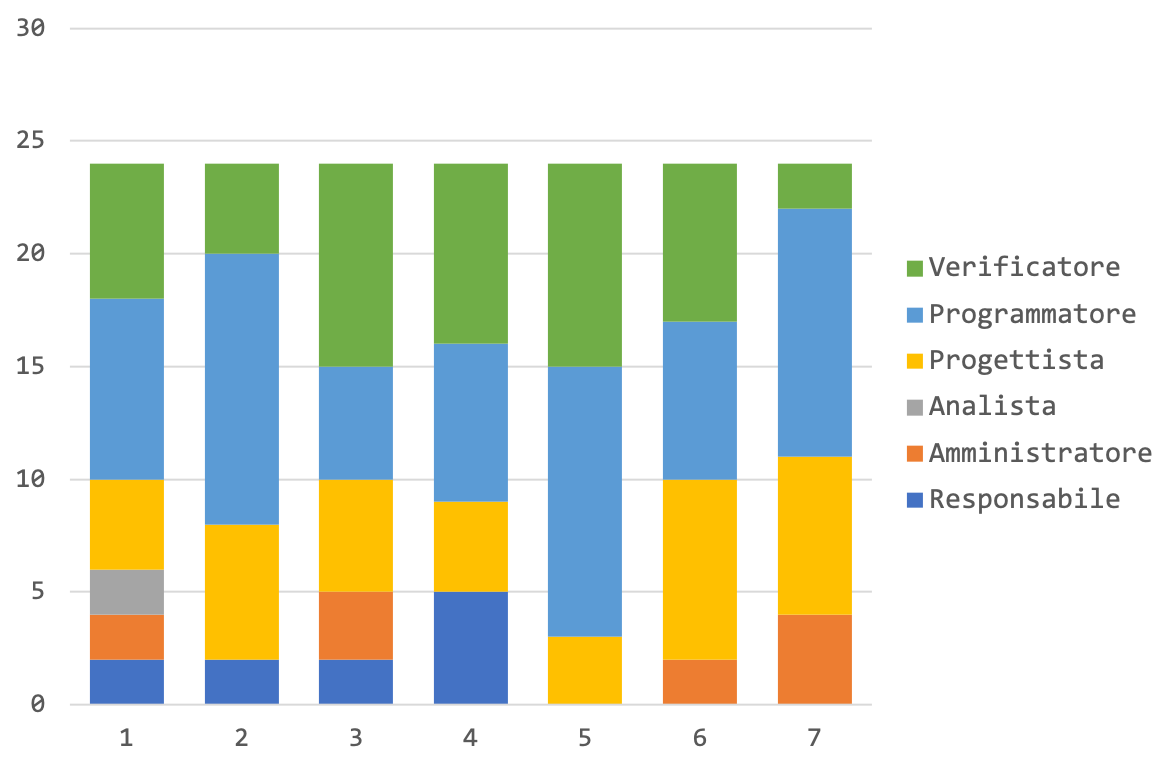
\includegraphics[width=0.8\linewidth]{./images/consuntivo/ConsIncr5-8-1.png}
			\caption{Diagramma ore/ruolo componenti dal quinto all'ottavo incremento}
			\label{fig:diagramma suddivione ruoli incrementi V-VIII}
		\end{figure}
		
		\paragraph{Riepilogo prospetto economico}
		In base al prospetto orario, quello economico sarà il seguente: 
		
		\rowcolors{2}{white}{lightest-grayest}
		\begin{longtable}{|l|c|c|}
			\hline
			\rowcolor{lighter-grayer}
			\textbf{Ruolo} & \textbf{Ore} & \textbf{Costo in € } \\
			\hline
			\endfirsthead
			
			\hline
			Responsabile 	    & 11 (+1) & 330,00 (+30,00)\\
			\hline 
			\hline
			Amministratore	   & 11 & 220,00\\
			\hline
			\hline
			Analista 				& 2 & 50,00\\
			\hline
			\hline
			Progettista 		   & 37 & 814,00\\
			\hline
			\hline
			Programmatore 	  & 62 (+3) & 885,00 (+45,00)\\
			\hline
			\hline
			Verificatore 		   & 45 (-4) & 675,00 (-60,00)\\
			\hline
			\textbf{Totale} 	 & 168 & 3019,00 (+15,00)\\
			\hline
			\caption{Tabella contenente il prospetto economico in riferimento al prospetto orario}
		\end{longtable}
		
		\pagebreak
		
		La tabella può essere riassunta nel seguente areogramma:
		\begin{figure}[H]
			\centering
			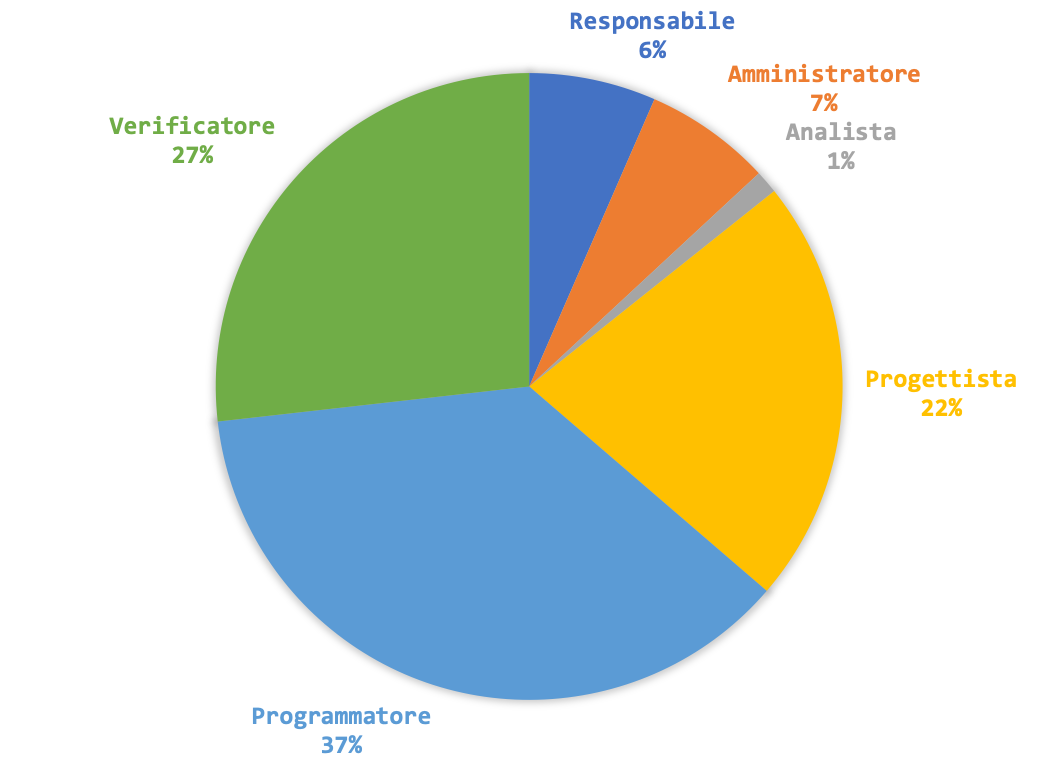
\includegraphics[width=0.8\linewidth]{./images/consuntivo/ConsIncr5-8-2.png}
			\caption{Diagramma consuntivo percentuale ore/ruolo dal quinto all'ottavo incremento}
			\label{fig:diagramma consuntivo costi ruolo incrementi V-VIII}
		\end{figure}
		
		\paragraph{Preventivo a finire}
		In questa prima fase, lo sviluppo del prodotto, sebbene leggermente altalenante per quanto riguarda le ore impiegate per i vari ruoli, è stato in linea con quanto preventivato inizialmente; di conseguenza il preventivo a finire resta invariato.
		\newline
		Infatti il gruppo è riuscito a realizzare tutte le funzionalità che aveva pianificato di implementare tramite gli incrementi e, grazie all'esperienza acquisita, confida di riuscire a recuperare la spesa di € 15,00, richiesta per consentire la variazione oraria necessaria, nei vari incrementi.
		
		\pagebreak
		
		\subsection{Completamento dell'implementazione e raffinamento delle funzionalità}
		I successivi quattro incrementi, che vedremo in dettaglio, comporranno la fase stessa.  		
		
		\subsubsection{Incremento IX}
			Le ore di lavoro di questo periodo sono volte all'implementazione della parte utente per la web app.
		\paragraph{Prospetto orario}
			La tabella seguente illustra il cambiamento nel numero d'ore di ogni persona, per ogni ruolo:
		
		\rowcolors{2}{lightest-grayest}{white}
		\begin{longtable}{|l|c|c|c|c|c|c|c|}
			\hline
			\rowcolor{lighter-grayer}
			\textbf{Nome} & \textbf{Re} & \textbf{Am} & \textbf{An} & \textbf{Pg}  & \textbf{Pr}   & \textbf{Ve} & \textbf{Totale} \\
			\hline
			\endfirsthead
			
			\hline
			Giuseppe Vito Bitetti 		 & 0 & 0 & 0 & 0 & 4 & 2 & 6\\
			\hline
			\hline
			Lorenzo Dei Negri			 & 0 & 0 & 0 & 2 & 0 & 4 & 6\\
			\hline
			\hline
			Nicolò Frison				      & 0 & 2 & 0 & 0 & 3 & 1 & 6\\
			\hline
			\hline
			Fouad Mouad 				   & 0 & 0 & 0 & 5 & 0 (-1) & 1 (+1) & 6\\
			\hline
			\hline
			Mariano Sciacco 			 & 0 & 0 & 0 & 2 & 2 (-2) & 2 (+2) & 6\\
			\hline
			\hline
			Alessandro Tommasin    & 0 & 0 & 0 & 2 & 4 & 0 & 6\\
			\hline
			\hline
			Giovanni Vidotto 			  & 4 & 0 & 0 & 0 & 2 & 0 & 6\\
			\hline 
			\textbf{Totale}			 		& 4 & 2 & 0 & 11 & 15 (-3) & 10 (+3) & 42\\
			\hline
			\caption{Tabella consuntiva contenente il prospetto orario per il nono incremento}
		\end{longtable}
		
		La tabella può essere riassunta nel seguente istogramma:
		
		\begin{figure}[H]
			\centering
			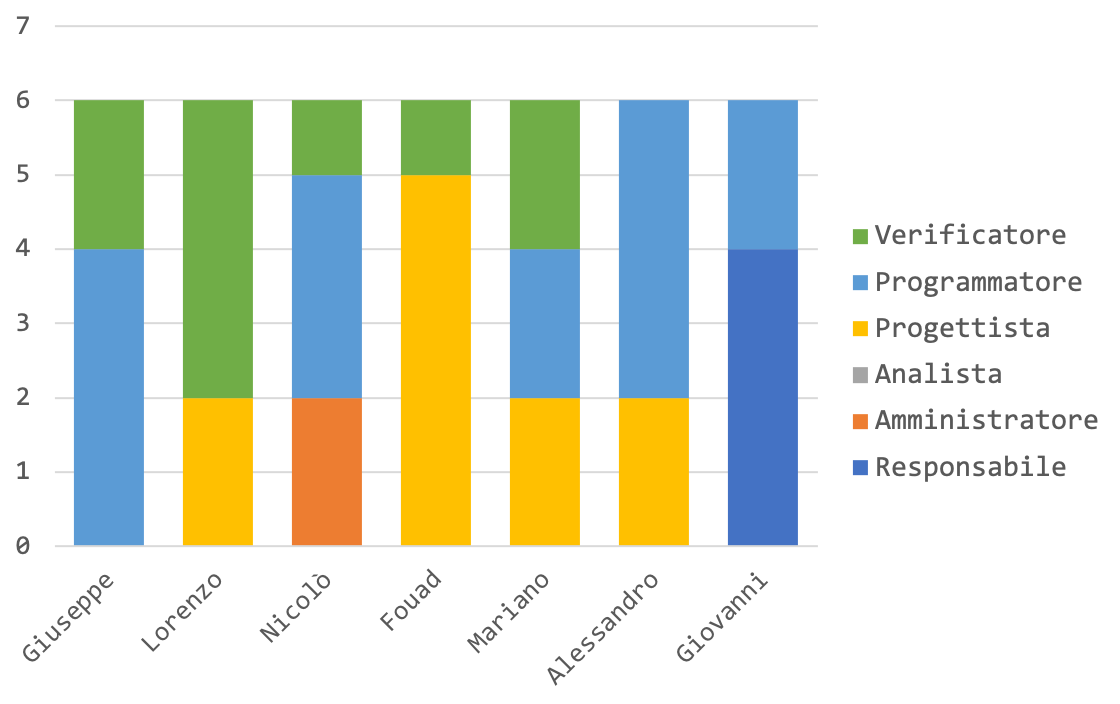
\includegraphics[width=0.7\linewidth]{images/consuntivo/ConsIncr9-1.png}
			\caption{Diagramma consuntivo ore/ruolo componenti dell'incremento IX}
			\label{fig:consuntivo diagramma suddivisione ruoli incremento IX}
		\end{figure}
		
		
		\paragraph{Prospetto economico}
			In base al prospetto orario, quello economico sarà il seguente: 
		
		\rowcolors{2}{white}{lightest-grayest}
		\begin{longtable}{|l|c|c|}
			\hline
			\rowcolor{lighter-grayer}
			\textbf{Ruolo} & \textbf{Ore} & \textbf{Costo in € } \\
			\hline
			\endfirsthead
			
			\hline
			Responsabile 	    & 4 & 120,00\\
			\hline 
			\hline
			Amministratore	   & 2 & 40,00\\
			\hline
			\hline
			Analista 				& 0 & 0,00\\
			\hline
			\hline
			Progettista 		   & 11 & 242,00\\
			\hline
			\hline
			Programmatore 	  & 15 (-3) & 225,00 (-45,00)\\
			\hline
			\hline
			Verificatore 		   & 10 (+3) & 150,00 (+45,00)\\
			\hline
			\textbf{Totale} 	 & 42 & 777,00\\
			\hline
			\caption{Tabella contenente il prospetto economico in riferimento al prospetto orario}
		\end{longtable}
		
		La tabella può essere riassunta nel seguente areogramma:
		\begin{figure}[H]
			\centering
			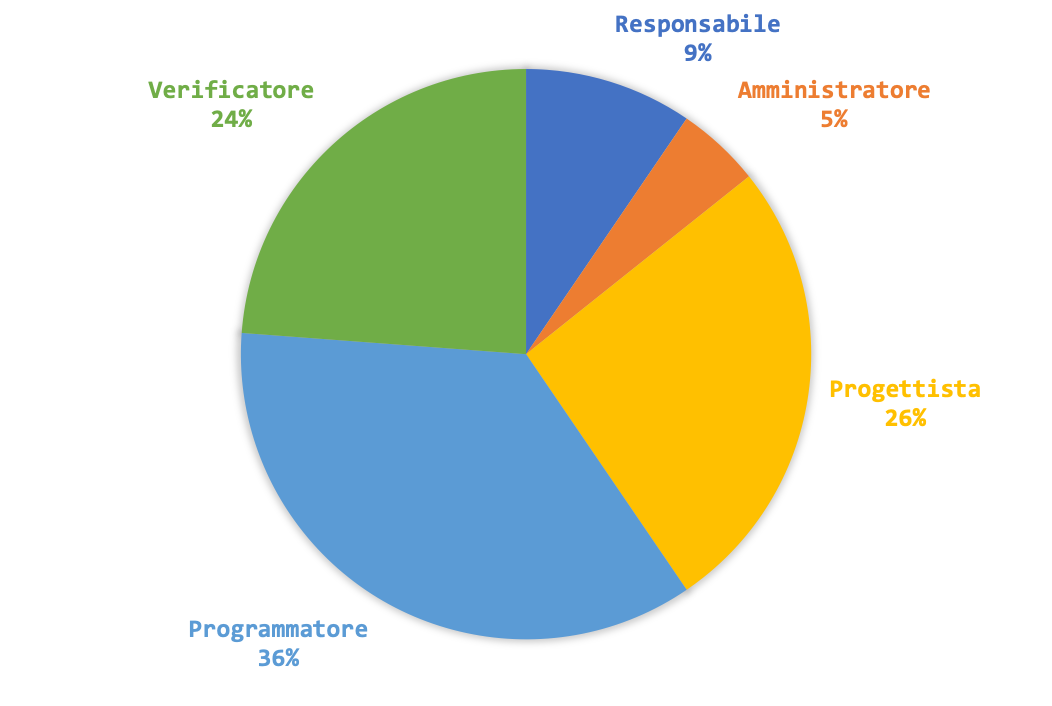
\includegraphics[width=0.8\linewidth]{images/consuntivo/ConsIncr9-2.png}
			\caption{Diagramma percentuale ore/ruolo nell'incremento IX}
			\label{fig:consuntivo diagramma costi ruolo incremento IX}
		\end{figure}
		\pagebreak
		\paragraph{Conclusioni}
			Durante l'incremento IX il gruppo ha lavorato mantenendo il numero di ore che erano state preventivate. È stato necessario però svolgere alcuni cambiamenti nella suddivisione oraria per ruolo, in particolare:
		\begin{itemize}
			\item \textbf{programmatore:} lo sviluppo della parte utente per la web app ha causato meno imprevisti rispetto a quelli preventivati e, alla luce di ciò, son state guadagnate tre ore che è stato possibile investire in fase di verifica;
			\item \textbf{verificatore:} il risparmio verificatosi nel ruolo del programmatore, ha reso possibile investire tre ore in più nel ruolo di verificatore.
		\end{itemize}
			Nonostante i cambiamenti effettuati il preventivo è rimasto invariato, investendo le stesso numero di ore che sono state preventivate.
		
		\paragraph{Preventivo a finire}
			Lo sviluppo procede in modo molto soddisfacente e, grazie alle ore risparmiate nella fase di programmazione, è stato possibile investire più risorse temporali per l'attività di verifica, nonostante fossero già state maggiorate nell'incremento precedente, in modo da equilibrare le ore spese per ogni componente del gruppo.
			\newline
			Come previsto al termine dell'incremento precedente, infatti, l'esperienza e le capacità acquisite dai componenti del gruppo ha permesso di risparmiare delle ore in codifica; queste ore sono state preventivamente impiegate nella verifica del software, in modo da assicurarne la qualità.
			\newline
			Nonostante la ridistribuzione oraria, il gruppo non ha accusato ulteriori spese rispetto a quelle preventivate, di conseguenza il preventivo a finire rimane in linea con quanto definito in \S5.
	
		\pagebreak
		
		\subsubsection{Incremento X}
			Le ore di lavoro svolte in questo periodo sono volte all'implementazione della moderazione per gli enti nella web app.
		
		\paragraph{Prospetto orario}
			Nella tabella in seguito viene illustrato il cambiamento nel numero d'ore di ogni persona, per ogni ruolo ricoperto:
			
			\rowcolors{2}{lightest-grayest}{white}
			\begin{longtable}{|l|c|c|c|c|c|c|c|}
				\hline
				\rowcolor{lighter-grayer}
				\textbf{Nome} & \textbf{Re} & \textbf{Am} & \textbf{An} & \textbf{Pg}  & \textbf{Pr}   & \textbf{Ve} & \textbf{Totale} \\
				\hline
				\endfirsthead
				
				\hline
				Giuseppe Vito Bitetti 		 & 0 & 0 & 0 & 3 & 0 & 3 & 6\\
				\hline
				\hline
				Lorenzo Dei Negri			 & 0 & 2 & 0 & 4 & 0 & 0 & 6\\
				\hline
				\hline
				Nicolò Frison				      & 0 & 0 & 0 & 3 & 0 & 3 & 6\\
				\hline
				\hline
				Fouad Mouad 				   & 0 & 0 & 0 & 0 & 4 & 2 & 6\\
				\hline
				\hline
				Mariano Sciacco 			 & 0 & 0 & 0 & 2 & 0 & 4 & 6\\
				\hline
				\hline
				Alessandro Tommasin    & 2 & 0 & 0 & 2 & 0 & 2 & 6\\
				\hline
				\hline
				Giovanni Vidotto 			  & 0 & 0 & 0 & 2 & 2 & 2 & 6\\
				\hline 
				\textbf{Totale}			 		& 2 & 2 & 0 & 16 & 6 & 16 & 42\\
				\hline
				\caption{Tabella consuntiva contenente il prospetto orario per il decimo incremento}
			\end{longtable}

			La tabella può essere riassunta nel seguente istogramma:
			\begin{figure}[H]
				\centering
				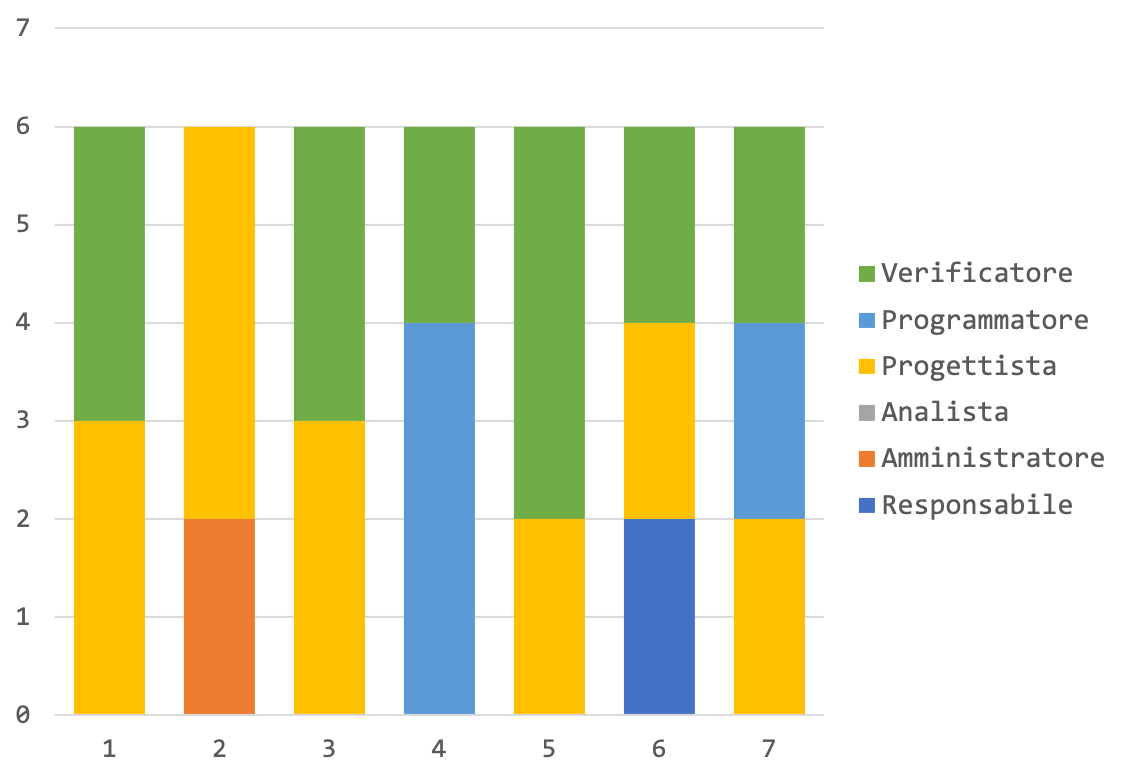
\includegraphics[width=0.8\linewidth]{./images/preventivo/incremento10-1.png}
				\caption{Diagramma consuntivo ore/ruolo componenti dell'incremento X}
				\label{fig:consuntivo diagramma suddivione ruoli incremento X}
			\end{figure}
			\pagebreak
			\paragraph{Prospetto economico}
			In base al prospetto orario, quello economico sarà il seguente: 
			
			\rowcolors{2}{white}{lightest-grayest}
			\begin{longtable}{|l|c|c|c|c|c|c|c|}
				\hline
				\rowcolor{lighter-grayer}
				\textbf{Ruolo} & \textbf{Ore} & \textbf{Costo in € } \\
				\hline
				\endfirsthead
				
				\hline
				Responsabile 	    & 2 & 60,00\\
				\hline 
				\hline
				Amministratore	   & 2 & 40,00\\
				\hline
				\hline
				Analista 				& 0 & 0,00\\
				\hline
				\hline
				Progettista 		   & 16 & 352,00\\
				\hline
				\hline
				Programmatore 	  & 6 & 90,00\\
				\hline
				\hline
				Verificatore 		   & 16 & 240,00\\
				\hline
				\textbf{Totale} 	 & 42 & 782,00\\
				\hline
				\caption{Tabella contenente il prospetto economico in riferimento al prospetto orario}
			\end{longtable}
			La tabella può essere riassunta nel seguente areogramma:
			\begin{figure}[H]
				\centering
				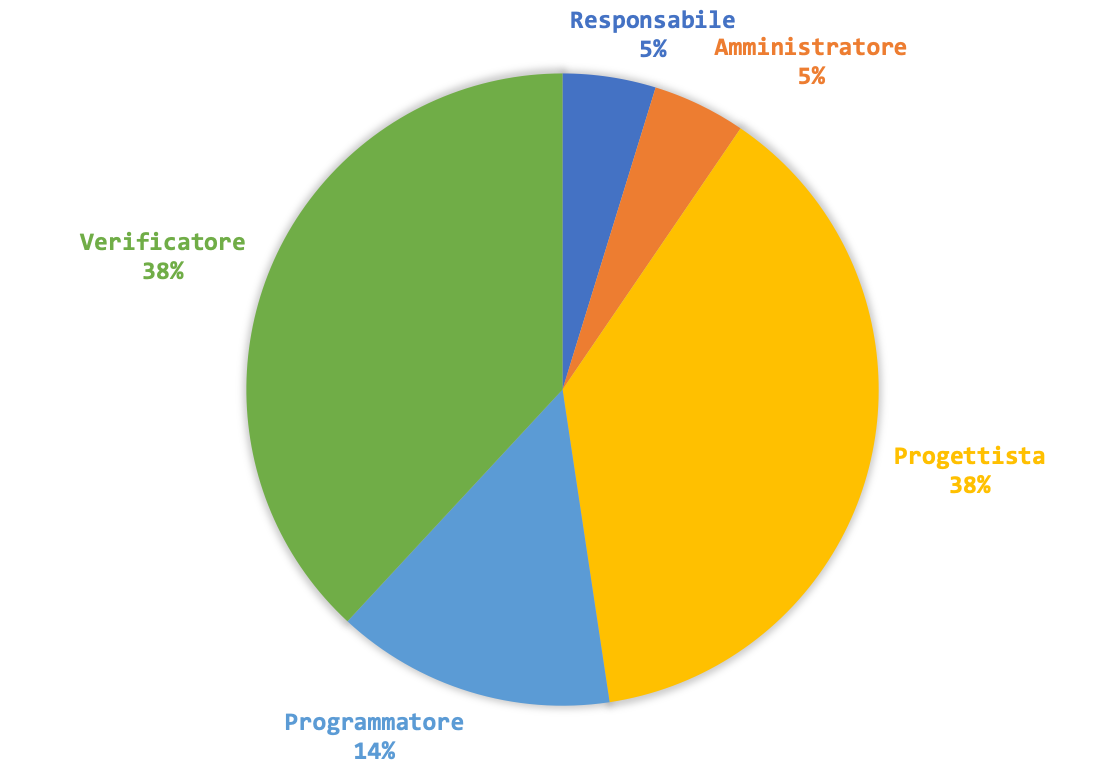
\includegraphics[width=0.8\linewidth]{./images/preventivo/incremento10-2.png}
				\caption{Diagramma percentuale ore/ruolo nell'ncremento X}
				\label{fig:consuntivo diagramma costi ruolo incremento X}
			\end{figure}
			\pagebreak
		
		\paragraph{Conclusioni}
			In questa fase non c'è stato alcun cambiamento orario rispetto alla suddivisione preventivata.
			Durante l'incremento il gruppo ha lavorato mantenendo il numero di ore che erano state preventivate. 
		
		\paragraph{Preventivo a finire}
			Lo sviluppo procede bene, le difficoltà riscontrate si sono rivelate in linea con quanto preventivato dal gruppo; infatti i membri avevano correttamente intuito la complessità degli ultimi incrementi, riuscendo quindi ad assegnare il giusto numero di ore ai diversi ruoli.
			\newline
			Considerando la tendenza positiva sperimentata fino a questo momento, il gruppo resta fiducioso per i prossimi due incrementi, nonostante siano più corposi e necessitino maggiori risorse temporali; di conseguenza il preventivo rimane in linea con quanto definito in \S5.
		\pagebreak
		
		%========================================================%
		
		\subsubsection{Incremento XI}
		Le ore di lavoro svolte in questo periodo sono volte all'implementazione completa delle \glock{API} e all'aggiunta dell'invio della configurazione ai \glock{gateway} con \glock{Kafka};
		\paragraph{Prospetto orario}
		Nella tabella in seguito viene illustrato il cambiamento nel numero d'ore di ogni persona, per ogni ruolo ricoperto:
		
		\rowcolors{2}{lightest-grayest}{white}
		\begin{longtable}{|l|c|c|c|c|c|c|c|}
			\hline
			\rowcolor{lighter-grayer}
			\textbf{Nome} & \textbf{Re} & \textbf{Am} & \textbf{An} & \textbf{Pg}  & \textbf{Pr}   & \textbf{Ve} & \textbf{Totale} \\
			\hline
			\endfirsthead
			
			\hline
			Giuseppe Vito Bitetti 		 & 0 & 0 & 0 & 0 & 0 (-3) & 6 (+3 )& 6\\
			\hline
			\hline
			Lorenzo Dei Negri			 & 0 & 2 & 0 & 0 & 3 & 1 & 6\\
			\hline
			\hline
			Nicolò Frison				      & 0 & 0 & 0 & 0 & 6 (+3) & 0 (-3) & 6\\
			\hline
			\hline
			Fouad Mouad 				   & 0 & 0 & 0 & 5 & 0 & 1 & 6\\
			\hline
			\hline
			Mariano Sciacco 			 & 0 & 0 & 0 & 2 & 4 & 0 & 6\\
			\hline
			\hline
			Alessandro Tommasin    & 2 & 0 & 0 & 2 & 0 & 2 & 6\\
			\hline
			\hline
			Giovanni Vidotto 			  & 0 & 0 & 0 & 1 (+1) & 3 (-1) & 2 & 6\\
			\hline 
			\textbf{Totale}			 		& 2 & 2 & 0 & 10 (+1) & 16 (-1) & 12 & 42\\
			\hline
			\caption{Tabella consuntiva contenente il prospetto orario per l'undicesimo incremento}
		\end{longtable}
		
		La tabella può essere riassunta nel seguente istogramma:
		\begin{figure}[H]
			\centering
			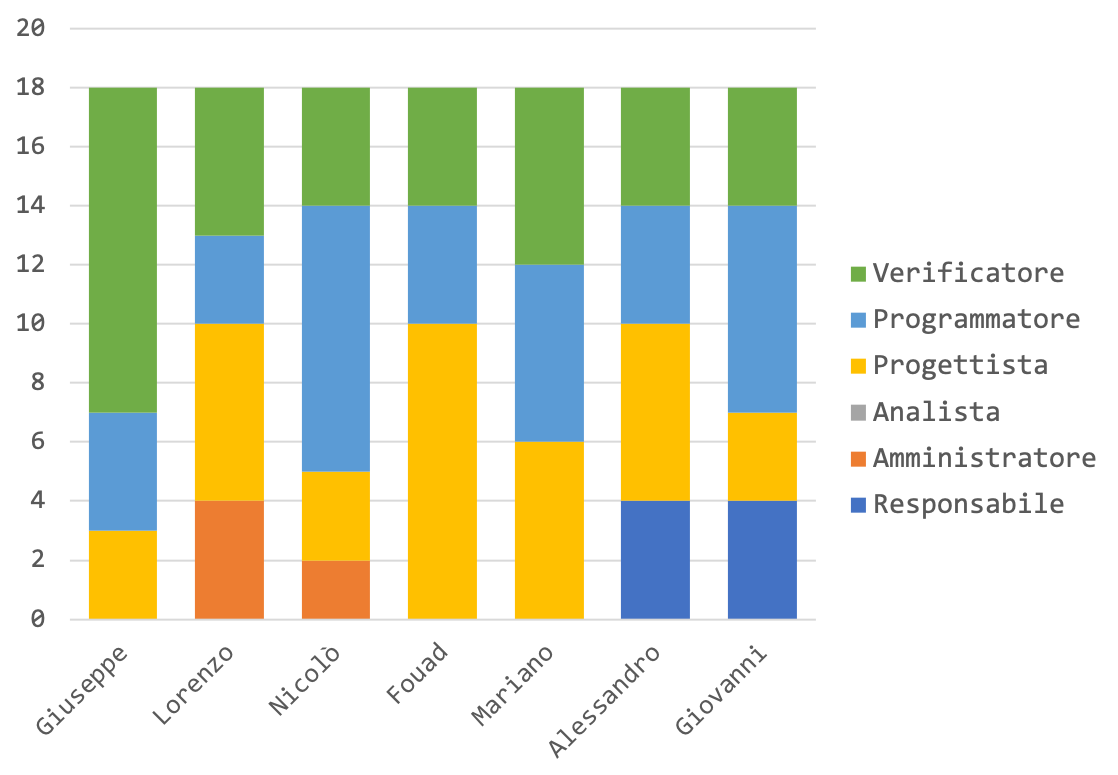
\includegraphics[width=0.8\linewidth]{./images/consuntivo/ConsIncr11-1.png}
			\caption{Diagramma consuntivo ore/ruolo componenti dell'incremento XI}
			\label{fig:consuntivo diagramma suddivione ruoli incremento XI}
		\end{figure}
		\pagebreak
		
		\paragraph{Prospetto economico}
		In base al prospetto orario, quello economico sarà il seguente: 
		
		\rowcolors{2}{white}{lightest-grayest}
		\begin{longtable}{|l|c|c|c|c|c|c|c|}
			\hline
			\rowcolor{lighter-grayer}
			\textbf{Ruolo} & \textbf{Ore} & \textbf{Costo in € } \\
			\hline
			\endfirsthead
			
			\hline
			Responsabile 	    & 2 & 60,00\\
			\hline 
			\hline
			Amministratore	   & 2 & 40,00\\
			\hline
			\hline
			Analista 				& - & -\\
			\hline
			\hline
			Progettista 		   & 10 (+1) & 220,00 (+22,00)\\
			\hline
			\hline
			Programmatore 	  & 16 (-1) & 240,00 (-15,00)\\
			\hline
			\hline
			Verificatore 		   & 16 & 240,00\\
			\hline
			\textbf{Totale} 	 & 42 & 740,00 (+7,00)\\
			\hline
			\caption{Tabella contenente il prospetto economico in riferimento al prospetto orario}
		\end{longtable}

		La tabella può essere riassunta nel seguente areogramma:
		\begin{figure}[H]
			\centering
			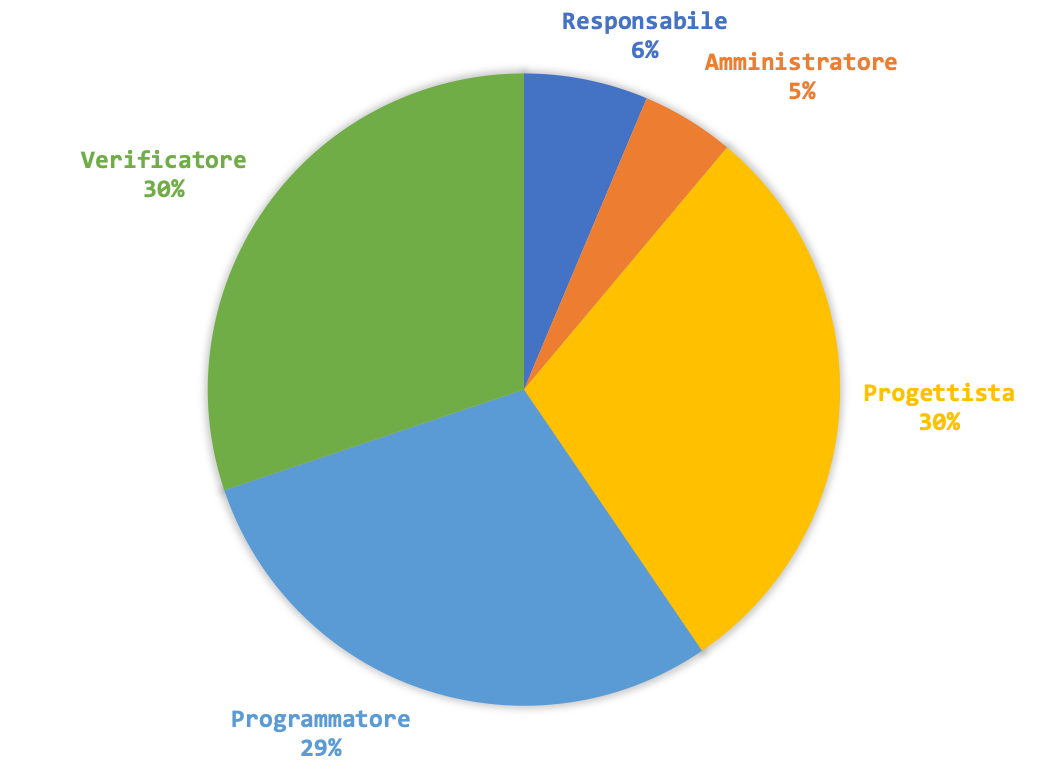
\includegraphics[width=0.8\linewidth]{./images/consuntivo/ConsIncr11-2.png}
			\caption{Diagramma percentuale ore/ruolo nell'incremento XI}
			\label{fig:consuntivo diagramma costi ruolo incremento XI}
		\end{figure}
		\pagebreak
		
		\paragraph{Conclusioni}
		Il gruppo è riuscito a mantenere invariato il numero di ore preventivato per l'incremento, tuttavia è stato necessario un minimo cambiamento nella suddivisione oraria per i ruoli di progettista e di programmatore. Infatti il design delle \glock{API} rimanenti ha richiesto più tempo del previsto, anche se poi la loro buona progettazione ne ha consentito un'implementazione più rapida, compensando il ritardo accumulato in precedenza.
		\newline
		Tutti gli altri obiettivi di sviluppo previsti per l'incremento sono stati raggiunti nel pieno rispetto dei tempi e dei costi pianificati.
		
		\paragraph{Preventivo a finire}
		Lo sviluppo procede in linea con quanto pianificato, nonostante il piccolo imprevisto verificatosi durante la progettazione delle API: il gruppo ha dovuto dedicare un'ora in più al design delle funzionalità, ma questa cura nella progettazione ha permesso, al momento dello sviluppo, di risparmiare un'ora di codifica, riportando così in pari il bilancio orario complessivo. 
		\newline
		Tutto ciò ha comportato un superamento di € 7,00 del costo totale preventivato, tuttavia, considerando che sono state realizzate tutte le funzionalità previste per l'incremento e che alla data attuale il gruppo registra un risparmio complessivo di € 15,00, non si ritiene necessario apportare modifiche al preventivo definito in \S5. Il team confida di concludere lo sviluppo con il prossimo incremento, rispettando la pianificazione.
				
		%==================================%
		
		\pagebreak
		
		\subsubsection{Incremento XII}
		Le ore di lavoro svolte in questo periodo sono volte all'implementazione dell'invio di comandi ai dispositivi tramite il \glock{bot Telegram} e della parte di amministratore all'interno della web app;
		\paragraph{Prospetto orario}
		Nella tabella in seguito viene illustrato il cambiamento nel numero d'ore di ogni persona, per ogni ruolo ricoperto:
		
		\rowcolors{2}{lightest-grayest}{white}
		\begin{longtable}{|l|c|c|c|c|c|c|c|}
			\hline
			\rowcolor{lighter-grayer}
			\textbf{Nome} & \textbf{Re} & \textbf{Am} & \textbf{An} & \textbf{Pg}  & \textbf{Pr}   & \textbf{Ve} & \textbf{Totale} \\
			\hline
			\endfirsthead
			
			\hline
			Giuseppe Vito Bitetti 		 & 0 & 0 & 0 & 4 & 0 & 6 & 10\\
			\hline
			\hline
			Lorenzo Dei Negri			 & 1 & 0 & 0 & 3 & 0 & 6 & 10\\
			\hline
			\hline
			Nicolò Frison				      & 0 & 0 & 0 & 4 & 3 & 3 & 10\\
			\hline
			\hline
			Fouad Mouad 				   & 0 & 0 & 0 & 2 & 2 (-3) & 6 (+3) & 10\\
			\hline
			\hline
			Mariano Sciacco 			 & 0 & 1 & 0 & 3 & 5 (+3) & 1 (-3) & 10\\
			\hline
			\hline
			Alessandro Tommasin    & 0 & 0 & 0 & 3 & 2 & 5 & 10\\
			\hline
			\hline
			Giovanni Vidotto 			  & 0 & 0 & 0 & 3 & 5 (+2) & 2 (-2) & 10\\
			\hline 
			\textbf{Totale}			 		& 1 & 1 & 0 & 22 & 17 (+2) & 29 (-2) & 70\\
			\hline
			\caption{Tabella consuntiva contenente il prospetto orario per il dodicesimo incremento}
		\end{longtable}

		La tabella può essere riassunta nel seguente istogramma:
		\begin{figure}[H]
			\centering
			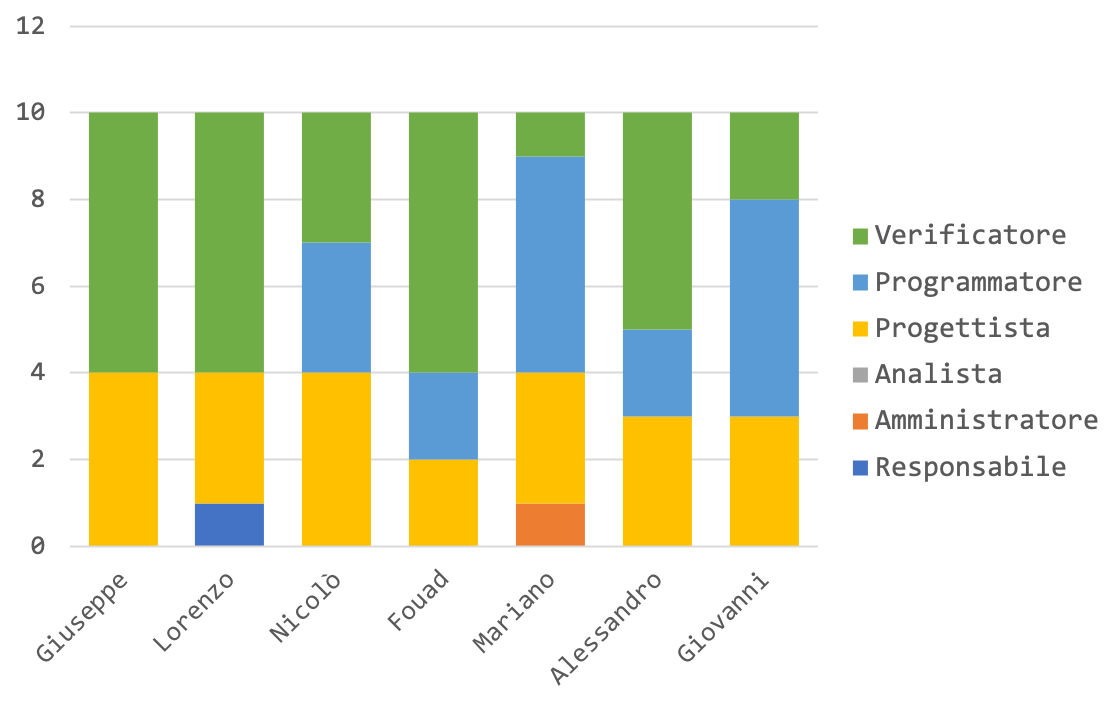
\includegraphics[width=0.8\linewidth]{./images/consuntivo/ConsIncr12-1.png}
			\caption{Diagramma consuntivo ore/ruolo componenti dell'incremento XII}
			\label{fig:consuntivo diagramma suddivione ruoli incremento XII}
		\end{figure}
		
		\paragraph{Prospetto economico}
		In base al prospetto orario, quello economico sarà il seguente: 
		
		\rowcolors{2}{white}{lightest-grayest}
		\begin{longtable}{|l|c|c|c|c|c|c|c|}
			\hline
			\rowcolor{lighter-grayer}
			\textbf{Ruolo} & \textbf{Ore} & \textbf{Costo in € } \\
			\hline
			\endfirsthead
			
			\hline
			Responsabile 	    & 1 & 30,00\\
			\hline 
			\hline
			Amministratore	   & 1 & 20,00\\
			\hline
			\hline
			Analista 				& - & - \\
			\hline
			\hline
			Progettista 		   & 22 & 484,00\\
			\hline
			\hline
			Programmatore 	  & 17 (+2) & 255,00 (+30,00)\\
			\hline
			\hline
			Verificatore 		   & 29 (-2) & 435,00 (-30,00)\\
			\hline
			\textbf{Totale} 	 & 70 & 1224,00\\
			\hline
			\caption{Tabella contenente il prospetto economico in riferimento al prospetto orario}
		\end{longtable}

		La tabella può essere riassunta nel seguente areogramma:
		\begin{figure}[H]
			\centering
			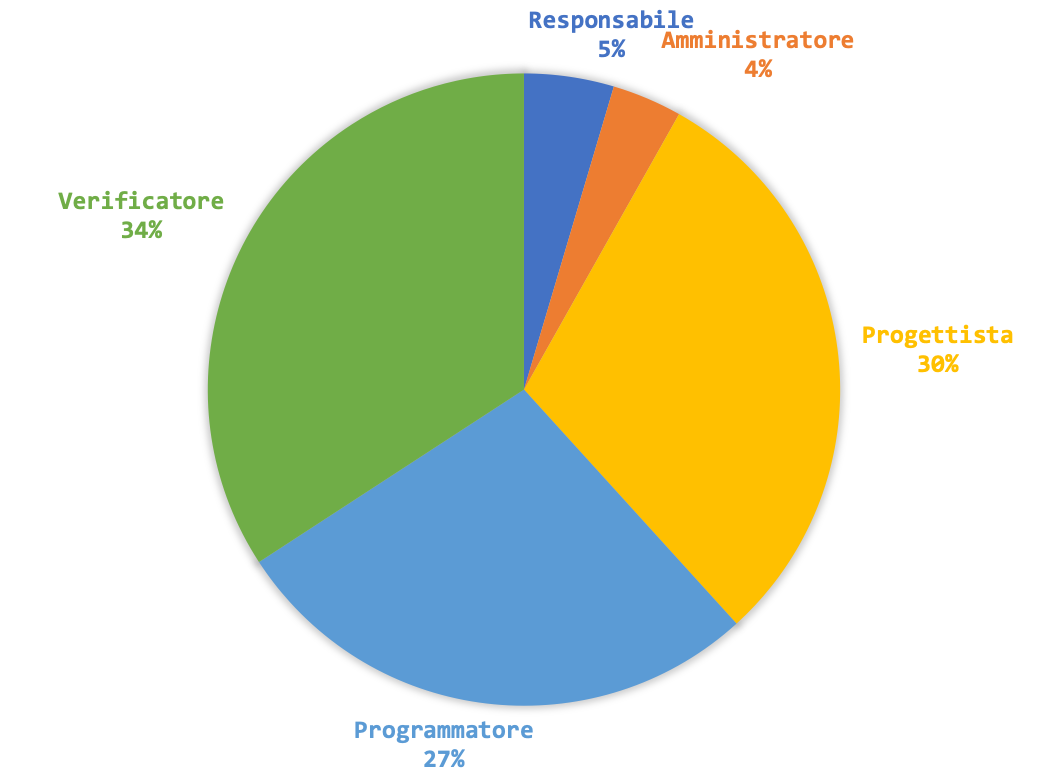
\includegraphics[width=0.8\linewidth]{./images/consuntivo/ConsIncr12-2.png}
			\caption{Diagramma percentuale ore/ruolo nell'incremento XII}
			\label{fig:consuntivo diagramma costi ruolo incremento XII}
		\end{figure}
		
		\pagebreak
		
		\paragraph{Conclusioni}
		Nonostante questo fosse l'incremento più lungo, il gruppo è riuscito a mantenere inalterato il numero di ore di lavoro previsto, limitandone i cambiamenti per ogni ruolo, grazie anche all'esperienza acquisita durante lo sviluppo del progetto.
		\newline
		Tuttavia, l'implementazione della funzionalità di invio dei comandi tramite il \glock{bot Telegram} ha richiesto ai programmatori più lavoro del previsto; questo è stato necessario per permettere l'inserimento di ulteriori istanze \glock{Axios} per la gestione delle richieste inviate dagli utenti.
		\newline
		Ciononostante, il tempo aggiuntivo ha consentito di curare di più la codifica, permettendo di velocizzare la verifica delle nuove parti implementate.
		
		\paragraph{Preventivo a finire}
		Con questo incremento si concludono le attività di codifica, e con esse anche lo sviluppo software. Il prodotto finale ottenuto offre tutte le funzionalità previste da pianificazione, di conseguenza il gruppo è molto soddisfatto.
		\newline
		Il completamento degli obiettivi di sviluppo dell'incremento ha richiesto due ore di codifica aggiuntive, recuperate però, in numero e costi, dal risparmio di altrettante ore di lavoro per i verificatori. Il bilancio risulta quindi in pari e il gruppo non ritiene necessario alcun intervento sul preventivo a finire, che rimane perciò in linea con quanto definito in \S5.
		\pagebreak
		
		%===================================%
		
		\subsubsection{Fase complessiva}
		
		\paragraph{Riepilogo prospetto orario}
		Dal nono al dodicesimo incremento la distribuzione oraria consuntiva dei ruoli di ogni componente del gruppo può essere riassunta nella seguente tabella:
			
			\rowcolors{2}{lightest-grayest}{white}
			\begin{longtable}{|l|c|c|c|c|c|c|c|}
				\hline
				\rowcolor{lighter-grayer}
				\textbf{Nome} & \textbf{Re} & \textbf{Am} & \textbf{An} & \textbf{Pg}  & \textbf{Pr}   & \textbf{Ve} & \textbf{Totale} \\
				\hline
				\endfirsthead
				
				\hline
				Giuseppe Vito Bitetti 		 & 0 & 0 & 0 & 3 & 4 & 5  & 12\\
				\hline
				\hline
				Lorenzo Dei Negri			 & 0 & 2 & 0 & 6 & 0 & 4 & 12\\
				\hline
				\hline
				Nicolò Frison				    & 0 & 2  & 0 & 3  & 3 & 4 & 12\\
				\hline
				\hline
				Fouad Mouad 				 & 0 & 0 & 0 & 5 & 4 (-1) & 3 (+1) & 12\\
				\hline
				\hline
				Mariano Sciacco 			 & 0 & 0 & 0 & 4 & 2 (-2) & 6 (+2) & 12\\
				\hline
				\hline
				Alessandro Tommasin     & 2 & 0 & 0 & 4 & 4 & 2 & 12\\
				\hline
				\hline
				Giovanni Vidotto 			 & 4 & 0 & 0 & 2 & 4 & 2 & 12\\
				\hline 
				\textbf{Totale}			 		& 6 & 4 & 0 & 27 & 21 (-3) & 26 (+3) & 84\\
				\hline
				\caption{Tabella contenente il prospetto orario consuntivo per gli ultimi quattro incrementi}
			\end{longtable}
			
			La tabella può essere riassunta nel seguente istogramma:
			\begin{figure}[H]
				\centering
				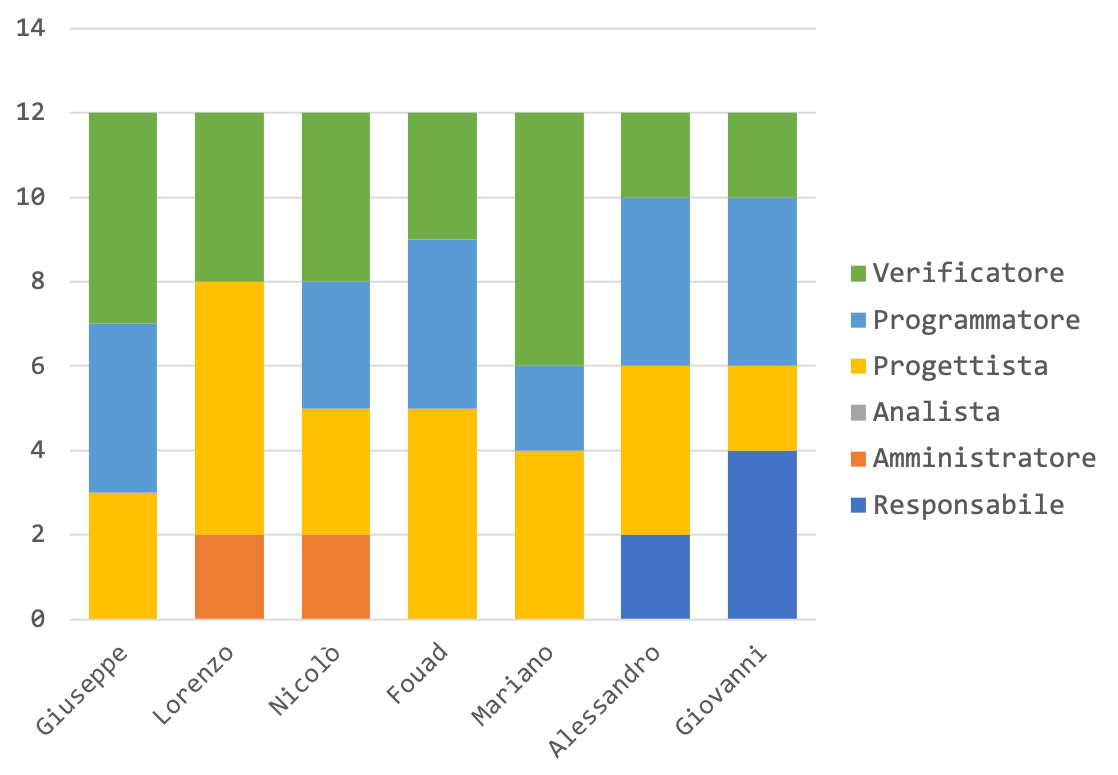
\includegraphics[width=0.8\linewidth]{./images/consuntivo/ConsIncr9-12-1.png}
				\caption{Diagramma ore/ruolo componenti negli ultimi quattro incrementi}
				\label{fig:diagramma suddivione ruoli incrementi IX-XII}
			\end{figure}
			
		
		\paragraph{Riepilogo prospetto economico}
			In base al prospetto orario, quello economico sarà il seguente: 
			
			\rowcolors{2}{white}{lightest-grayest}
			\begin{longtable}{|l|c|c|}
				\hline
				\rowcolor{lighter-grayer}
				\textbf{Ruolo} & \textbf{Ore} & \textbf{Costo in € } \\
				\hline
				\endfirsthead
				
				\hline
				Responsabile 	    & 6 & 180,00\\
				\hline 
				\hline
				Amministratore	   & 4 & 80,00\\
				\hline
				\hline
				Analista 				& - & -\\
				\hline
				\hline
				Progettista 		   & 27 & 594,00\\
				\hline
				\hline
				Programmatore 	  & 21 (-3)  & 315,00 (-45,00)\\
				\hline
				\hline
				Verificatore 		   & 26 (+3) & 390,00 (+45,00)\\
				\hline
				\textbf{Totale} 	 & 84 & 1559,00\\
				\hline
				\caption{Tabella contenente il prospetto economico in riferimento al prospetto orario}
			\end{longtable}
			
			La tabella può essere riassunta nel seguente areogramma:
			\begin{figure}[H]
				\centering
				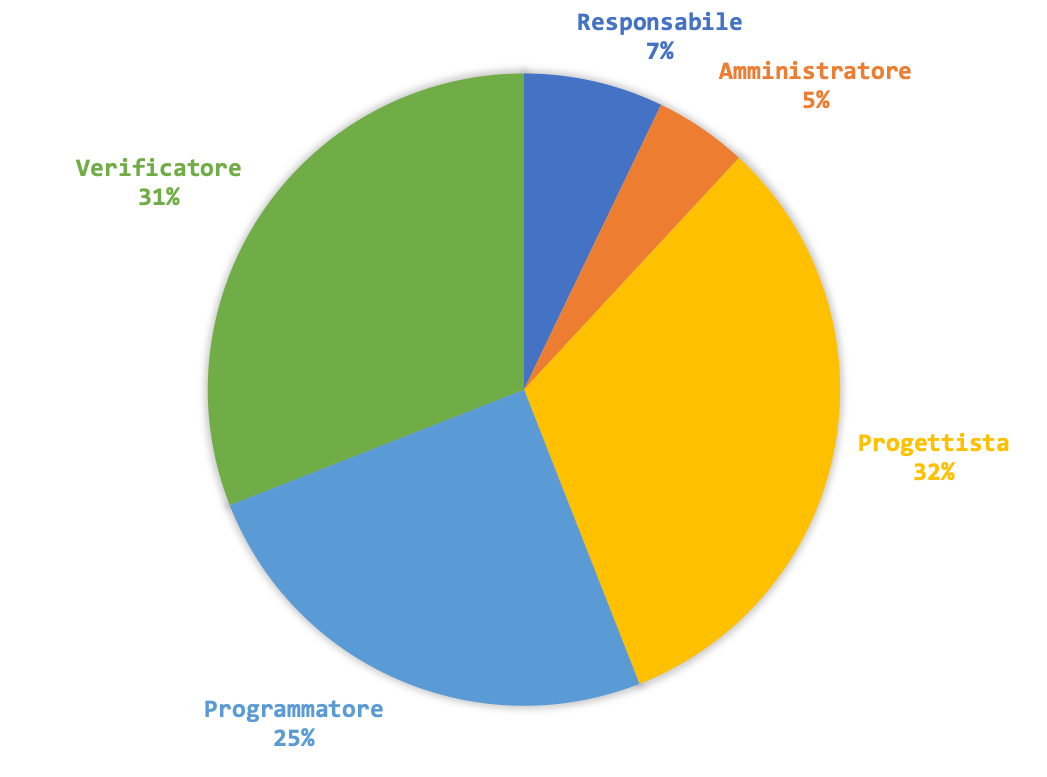
\includegraphics[width=0.8\linewidth]{./images/consuntivo/ConsIncr9-12-2.png}
				\caption{Diagramma consuntivo percentuale ore/ruolo degli ultimi quattro incrementi}
				\label{fig:diagramma consuntivo costi ruolo incrementi IX-XII}
			\end{figure}
		\pagebreak
		\paragraph{Preventivo a finire}
			Durante questo periodo sono state completamente implementate e raffinate le funzionalità di tutte le componenti del prodotto. Il lavoro svolto ha portato ad un risultato al di sopra delle aspettative iniziali del gruppo, che si ritiene quindi molto soddisfatto.
			\newline
			La consegna del prodotto ai committenti è stata fissata per il giorno 15 maggio 2020, tre giorni prima della data di fine progetto. Poiché la pianificazione attuale prevede di terminare la fase di validazione e collaudo il giorno 17 maggio 2020, il gruppo ha deciso di anticipare il completamento di tutte le attività che coinvolgeranno documenti e prodotto software entro il giorno 15 maggio 2020; il consuntivo finale sarà compilato in tale data.
			\newline
			Nonostante i cambiamenti effettuati durante i singoli incrementi, il consuntivo di fine fase riporta un quadro abbastanza in linea con quanto preventivato. Il monte ore complessivo è rimasto invariato rispetto alla pianificazione, a discapito di una spesa maggiorata di € 7,00; questa però è stata mitigata dai € 15,00 che erano stati risparmiati nella fase precedente.
			\newline
			Di conseguenza non si ritiene necessario intervenire sul preventivo definito in \S5, a meno della variazione esposta in precedenza per consentire la consegna del prodotto entro i termini stabiliti.
			
		%=================================================================%
		
		\pagebreak
		
		\subsection{Fase di validazione e collaudo}
		Le ore di lavoro del periodo sono volte alla conclusione dei manuali, ai controlli di qualità e validazione dei prodotti software e documentali ed al rilascio dell'ultima versione del prodotto completo.

		\subsubsection{Prospetto orario}
		La tabella seguente illustra il cambiamento nel numero d'ore di ogni persona, per ogni ruolo:
		
		\rowcolors{2}{lightest-grayest}{white}
		\begin{longtable}{|p{3.5cm}|c|c|c|c|c|c|c|}
			\hline
			\rowcolor{lighter-grayer}
			\textbf{Nome} & \textbf{Re} & \textbf{Am} & \textbf{An} & \textbf{Pg}  & \textbf{Pr}   & \textbf{Ve} & \textbf{Totale} \\
			\hline
			\endfirsthead
			
			\hline
			Giuseppe Vito Bitetti 		 & 1(+1) & 2(-1) & 2 & 0 & 4 & 7(+1) & 16(+1)\\
			\hline
			\hline
			Lorenzo Dei Negri			 & 3(-2) & 0 & 0 & 3 & 5 & 5(+3) & 16(+1)\\
			\hline
			\hline
			Nicolò Frison				      & 0 & 2(-2) & 4 & 1 & 5(+3) & 4 & 16(+1)\\
			\hline
			\hline
			Fouad Mouad 				   & 5 & 0 & 2 & 0 & 0 & 9(+1) & 16(+1)\\
			\hline
			\hline
			Mariano Sciacco 			 & 0 & 5(-1) & 2 & 2 & 5 & 2(+2) & 16(+1)\\
			\hline
			\hline
			Alessandro Tommasin    & 2(-3) & 0 & 3  & 3(-1) & 4(+4) & 4(+1) & 16(+1)\\
			\hline
			\hline
			Giovanni Vidotto 			  & 0 & 4(-2) & 3 & 2 & 4(+2) & 3(+1) & 16(+1)\\
			\hline 
			\textbf{Totale}			 	& 12(-3) & 13(-6) & 16 & 11(-1) & 26(+8) & 34(+9) & 112(+7)\\
			\hline
			\caption{Tabella contenente il prospetto orario preventivato per la fase di validazione e collaudo}
		\end{longtable}

		La tabella può essere riassunta nel seguente istogramma:
		\begin{figure}[H]
			\centering
			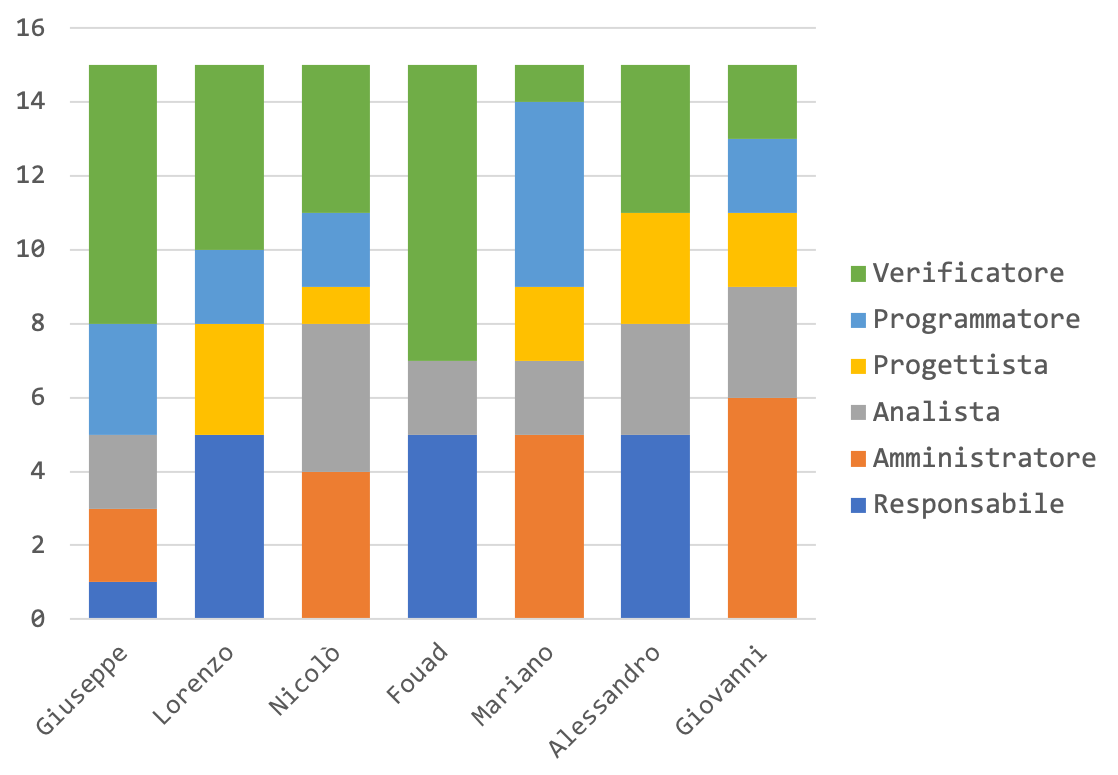
\includegraphics[width=0.75\linewidth]{./images/consuntivo/validCollCons1.png}
			\caption{Diagramma ore/ruolo componenti nella fase di validazione e collaudo}
			\label{fig:diagramma suddivione ruoli fase di validazione e collaudo}
		\end{figure}

		\subsubsection{Prospetto economico}
		In base al prospetto orario, quello economico sarà il seguente: 
		
		\rowcolors{2}{white}{lightest-grayest}
		\begin{longtable}{|l|c|c|c|c|c|c|c|}
			\hline
			\rowcolor{lighter-grayer}
			\textbf{Ruolo} & \textbf{Ore} & \textbf{Costo in € } \\
			\hline
			\endfirsthead
			
			\hline
			Responsabile 	    & 11 (-4) & 330,00 (-120,00)\\
			\hline 
			\hline
			Amministratore	   & 13 (-6) & 260,00 (-120,00)\\
			\hline
			\hline
			Analista 				& 16 & 400,00\\
			\hline
			\hline
			Progettista 		   & 11 (-1) & 242,00 (-22,00)\\
			\hline
			\hline
			Programmatore 	  & 27 (+9) & 405,00 (+135,00)\\
			\hline
			\hline
			Verificatore 		   & 34 (+9) & 510,00 (+135,00)\\
			\hline
			\textbf{Totale} 	 & 112 (+7 )& 2.147,00 (+8,00)\\
			\hline
			\caption{Tabella contenente il prospetto economico in riferimento al prospetto orario}
		\end{longtable}
		
		La tabella può essere riassunta nel seguente areogramma:
		\begin{figure}[H]
			\centering
			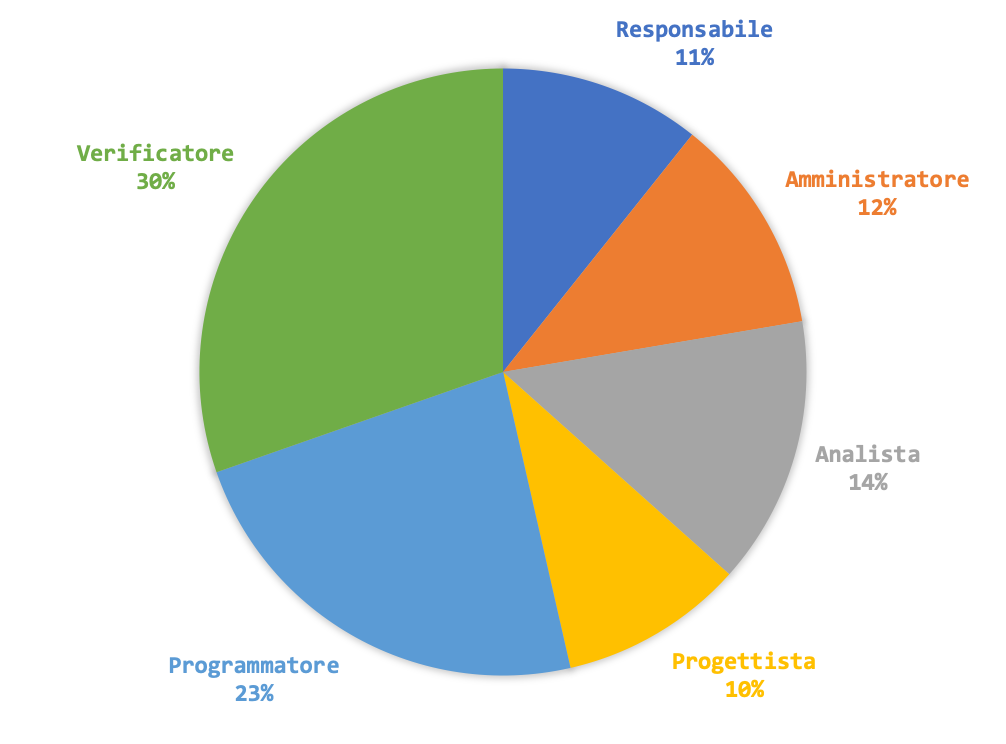
\includegraphics[width=0.8\linewidth]{./images/consuntivo/validCollCons2.png}
			\caption{Diagramma percentuale ore/ruolo della fase di validazione e collaudo}
			\label{fig:diagramma costi ruolo fase di validazione e collaudo}
		\end{figure}	
		
		\pagebreak
		
		\subsubsection{Conclusioni}
		In quest'ultima fase, in seguito alle segnalazioni fatte dai committenti in sede di revisione di qualifica, è stato necessario intervenire profondamente sulla struttura e sui contenuti del manuale utente. La scelta del gruppo di sostituire le sezioni illustrative delle funzionalità con degli appositi video tutorial si è rivelata inadeguata, quindi si è dovuto passare ad una stesura del manuale più tradizionale. Le informazioni contenute nei video sono state trascritte con il supporto di opportune immagini esplicative delle funzionalità trattate.
		\newline
		Questa attività ha comportato uno sforzo imprevisto per la redazione e conseguente verifica del documento.	Tuttavia, il gruppo è riuscito a completare le restanti attività previste, senza ulteriori deviazioni rispetto alla pianificazione iniziale.
		
		\subsubsection{Preventivo a finire}
		Per completare la nuova stesura del manuale utente sono state necessarie 9 ore di lavoro in più per i programmatori e altrettante in più per i verificatori. Il gruppo ha allora lavorato per compensare questo eccesso velocizzando il più possibile le attività legate agli altri ruoli. Sono state quindi risparmiate 4 ore, 6 ore e 1 ora rispettivamente di responsabile, amministratore e progettista. Le 7 ore rimaste scoperte sono state distribuite equamente tra tutti i componenti del gruppo, in pieno rispetto della regola, fissata dal team ad inizio progetto, di svolgere tutti lo stesso numero di ore per ogni fase.
		\newline
		In seguito a questa ridistribuzione oraria, è stata superata di € 8,00 la somma totale preventivata per la fase appena conclusa. Tuttavia, questo eccesso va a pareggiare gli € 8,00 risparmiati in precedenza. Il bilancio complessivo rendicontato risulta quindi in pari.
		
		\pagebreak
		
		%=================================================================%
		
		\subsection{Riepilogo ore totali}
		\subsubsection{Totale ore complessive}
		\paragraph{Totale prospetto orario complessivo}
		Riepilogo della distribuzione oraria di tutte le fasi:
		\rowcolors{2}{lightest-grayest}{white}
		\begin{longtable}{|p{1.725cm}|p{1.1cm}|p{1.1cm}|p{1.1cm}|p{1.1cm}|p{1.1cm}|p{1.1cm}|p{1.1cm}|}
			\hline
			\rowcolor{lighter-grayer}
			\textbf{Nome} & \textbf{Re} & \textbf{Am} & \textbf{An} & \textbf{Pg}  & \textbf{Pr}   & \textbf{Ve} & \textbf{Totale} \\
			\hline
			\endfirsthead
			
			\hline
			Giuseppe Vito Bitetti 		& 8 & 12 (-2) & 29 (+1) & 15 (+1) & 25 (-1) & 50 (+2) & 139 (+1)\\
			\hline
			Lorenzo Dei Negri			& 14 (-4) & 14 & 15 (+1) & 28 (-2) & 23 & 45 (+6) & 139 (+1)\\
			\hline
			Nicolò Frison				    & 8 & 20 (-5) & 18 (+1) & 21 (-1) & 29 (+6) & 43 & 139 (+1)\\
			\hline
			Fouad Mouad 				 & 14 & 17 & 21 & 22 (+1) & 16 (-5) & 49 (+5) & 139 (+1)\\
			\hline
			Mariano Sciacco 			& 14 & 9\newline(-1) & 18 & 28 (+1) & 36 (+2) & 34 (-1) & 139 (+1)\\
			\hline
			Alessandro Tommasin    & 15 (-5) & 9 & 28 (+3) & 25 (-3) & 24 (+6) & 38 & 139 (+1)\\
			\hline
			Giovanni Vidotto 			 & 8 & 16 (-3) & 17 (+1) & 29 (+3) & 31 (+2) & 38 (-2) & 139 (+1)\\
			\hline 
			\textbf{Totale}				 & 81 (-9) & 97 (-11) & 146 (+7) & 168 & 184 (+10) & 297 (+10) & 973 (+7)\\
			\hline
			\caption{Tabella contenente il prospetto orario riepilogativo di tutti i periodi trattati in precedenza}
		\end{longtable}
		
		\pagebreak
		
		La tabella può essere riassunta nel seguente istogramma:
		\begin{figure}[H]
			\centering
			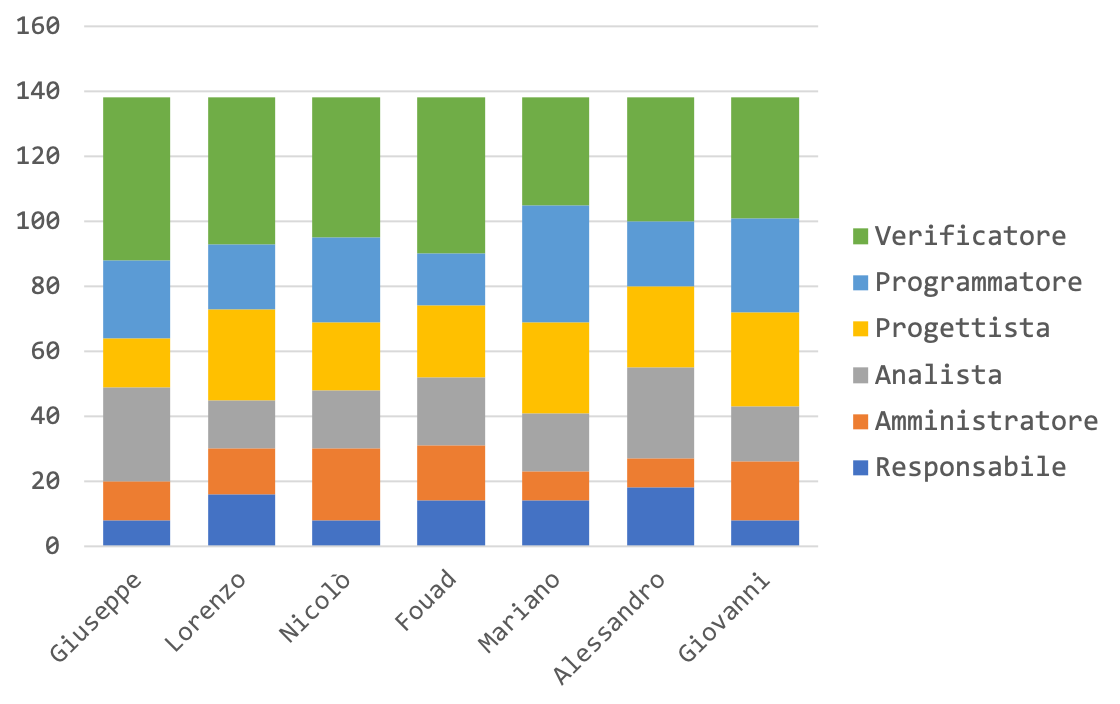
\includegraphics[width=0.8\linewidth]{./images/consuntivo/totOre1.png}
			\caption{Diagramma ore/ruolo componenti nel totale delle ore}
			\label{fig:diagramma suddivione ruoli totale ore}
		\end{figure}
		
		\paragraph{Totale prospetto economico complessivo}
		In base al prospetto orario, quello economico sarà il seguente: 
		
		\rowcolors{2}{white}{lightest-grayest}
		\begin{longtable}{|l|c|c|c|c|c|c|c|}
			\hline
			\rowcolor{lighter-grayer}
			\textbf{Ruolo} & \textbf{Ore} & \textbf{Costo in € } \\
			\hline
			\endfirsthead
			
			\hline
			Responsabile 	    & 821 (-9) & 2.430,00 (-270,00)\\
			\hline 
			\hline
			Amministratore	  & 97 (-11) & 1.940,00 (-220,00)\\
			\hline
			\hline
			Analista 				& 146 (+7) & 3.650,00 (+175,00)\\
			\hline
			\hline
			Progettista 		  & 168 & 3.696,00\\
			\hline
			\hline
			Programmatore 	 & 184 (+10) & 2.760,00 (+150,00)\\
			\hline
			\hline
			Verificatore 		  & 297 (+10) & 4.455,00 (+150,00)\\
			\hline
			\textbf{Totale} 	& 973 (+7) & 18.931,00 \\
			\hline
			\caption{Tabella contenente il prospetto economico in riferimento al prospetto orario}
		\end{longtable}
		
		\pagebreak
		
		La tabella può essere riassunta nel seguente areogramma:
		\begin{figure}[H]
			\centering
			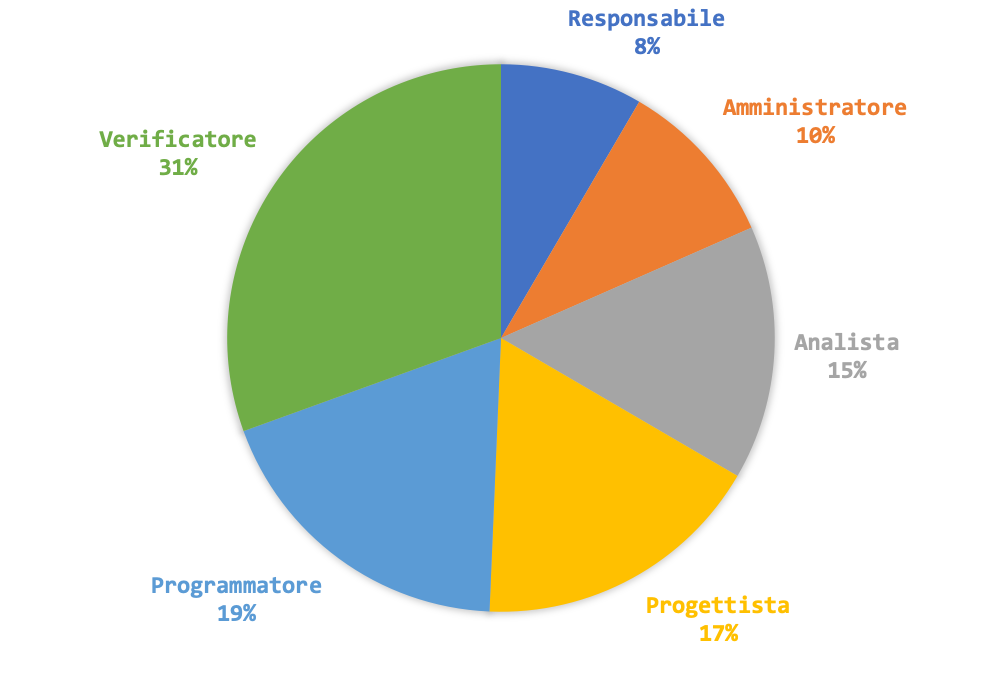
\includegraphics[width=0.8\linewidth]{./images/consuntivo/totOre2.png}
			\caption{Diagramma percentuale ore/ruolo nel totale delle ore}
			\label{fig:diagramma costi ruolo fase totale ore}
		\end{figure}
		
		\pagebreak
		
		\subsubsection{Totale ore rendicontate}
		\paragraph{Totale prospetto orario rendicontato}
		Riepilogo della distribuzione oraria delle fasi a carico del committente, escludendo quindi le fasi di analisi e consolidamento dei requisiti:
		
		\rowcolors{2}{lightest-grayest}{white}
		\begin{longtable}{|p{1.725cm}|c|c|c|c|c|c|c|}
			\hline
			\rowcolor{lighter-grayer}
			\textbf{Nome} & \textbf{Re} & \textbf{Am} & \textbf{An} & \textbf{Pg}  & \textbf{Pr}   & \textbf{Ve} & \textbf{Totale} \\
			\hline
			\endfirsthead
			
			\hline
			Giuseppe Vito Bitetti 		& 8 & 4(-1) & 14 & 15(+1) & 25(-1) & 38(+2) & 104(+1)\\
			\hline
			\hline
			Lorenzo Dei Negri			& 8(-2)  & 9 & 1 & 28(-2) & 23 & 35(+5) & 104(+1)\\
			\hline
			\hline
			Nicolò Frison				    & 8 & 12(-3) & 9 & 21(-1) & 28(+5) & 25(-1) & 104(+1)\\
			\hline
			\hline
			Fouad Mouad 				 & 13(+1) & 10 & 9(-1) & 22(+1) & 16(-5) & 34(+5) & 104(+1)\\
			\hline
			\hline
			Mariano Sciacco 			& 6 & 9(-1) & 3 & 28(+1) & 36(+2) & 22(-1) & 104(+1)\\
			\hline
			\hline
			Alessandro Tommasin    & 6(-3) & 9 & 11 & 25(-3) & 24(+6) & 29(+1) & 104(+1)\\
			\hline
			\hline
			Giovanni Vidotto 			 & 6 & 10(-2) & 8 & 29(+3) & 31(+2) & 20(-2) & 104(+1)\\
			\hline 
			\textbf{Totale}				 & 56(-3) & 63(-7) & 55(-1) & 168 & 183(+9) & 203(+9) & 728(+7)\\
			\hline
			\caption{Tabella contenente il prospetto orario preventivato a carico del committente}
		\end{longtable}
		
		\pagebreak
		
		La tabella può essere riassunta nel seguente istogramma:
		\begin{figure}[H]
			\centering
			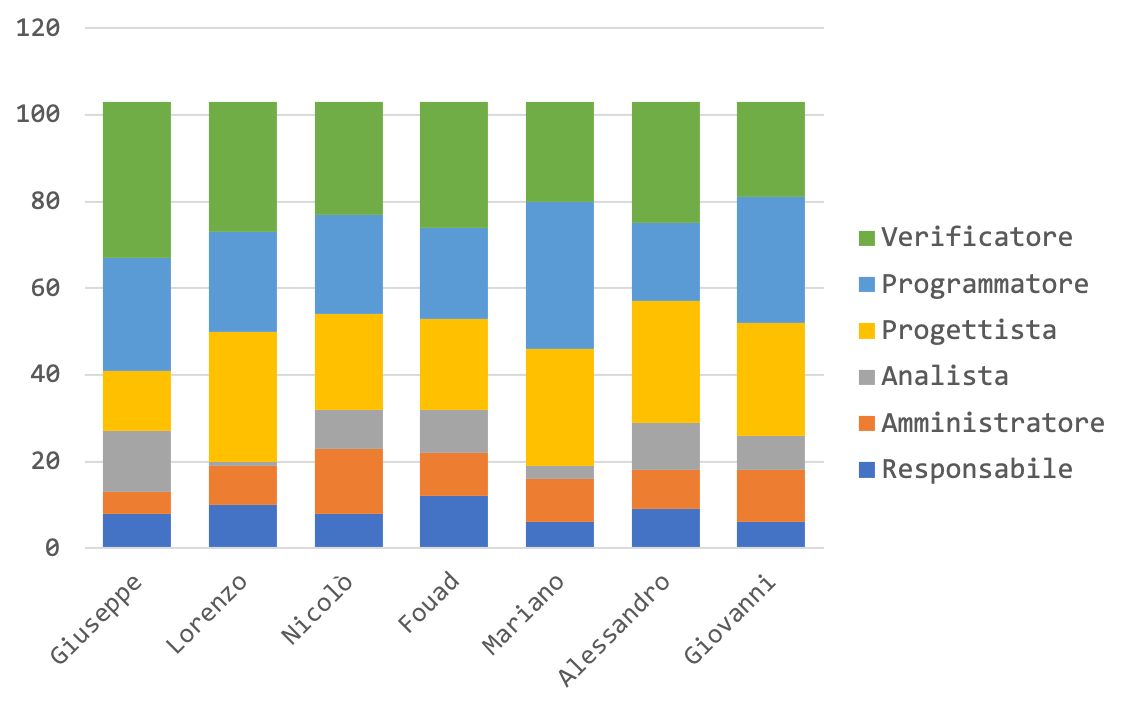
\includegraphics[width=0.8\linewidth]{./images/preventivo/totOreRed1.png}
			\caption{Diagramma ore/ruolo componenti nel totale delle ore rendicontate}
			\label{fig:diagramma suddivione ruoli totale ore rendicontete}
		\end{figure}
		
		\paragraph{Totale prospetto economico rendicontato}
		In base al prospetto orario, quello economico sarà il seguente: 
		
		\rowcolors{2}{white}{lightest-grayest}
		\begin{longtable}{|l|c|c|c|c|c|c|c|}
			\hline
			\rowcolor{lighter-grayer}
			\textbf{Ruolo} & \textbf{Ore} & \textbf{Costo in €} \\
			\hline
			\endfirsthead
			
			\hline
			Responsabile 	    & 55 (-4) & 1.650,00 (-120,00)\\
			\hline 
			\hline
			Amministratore	  & 63 (-7) & 1.260,00 (-140,00)\\
			\hline
			\hline
			Analista 				& 55 (-1) & 1.375,00 (-25,00)\\
			\hline
			\hline
			Progettista 		  & 168 & 3.696,00\\
			\hline
			\hline
			Programmatore 	 & 184 (+10) & 2.760,00 (+150,00)\\
			\hline
			\hline
			Verificatore 		  & 203 (+9) & 3.045,00 (+135,00)\\
			\hline
			\textbf{Totale} 	& 728 (+7) & 13.786,00\\
			\hline
			\caption{Tabella contenente il prospetto economico in riferimento al prospetto orario}
		\end{longtable}
		
		\pagebreak
		
		La tabella può essere riassunta nel seguente areogramma:
		\begin{figure}[H]
			\centering
			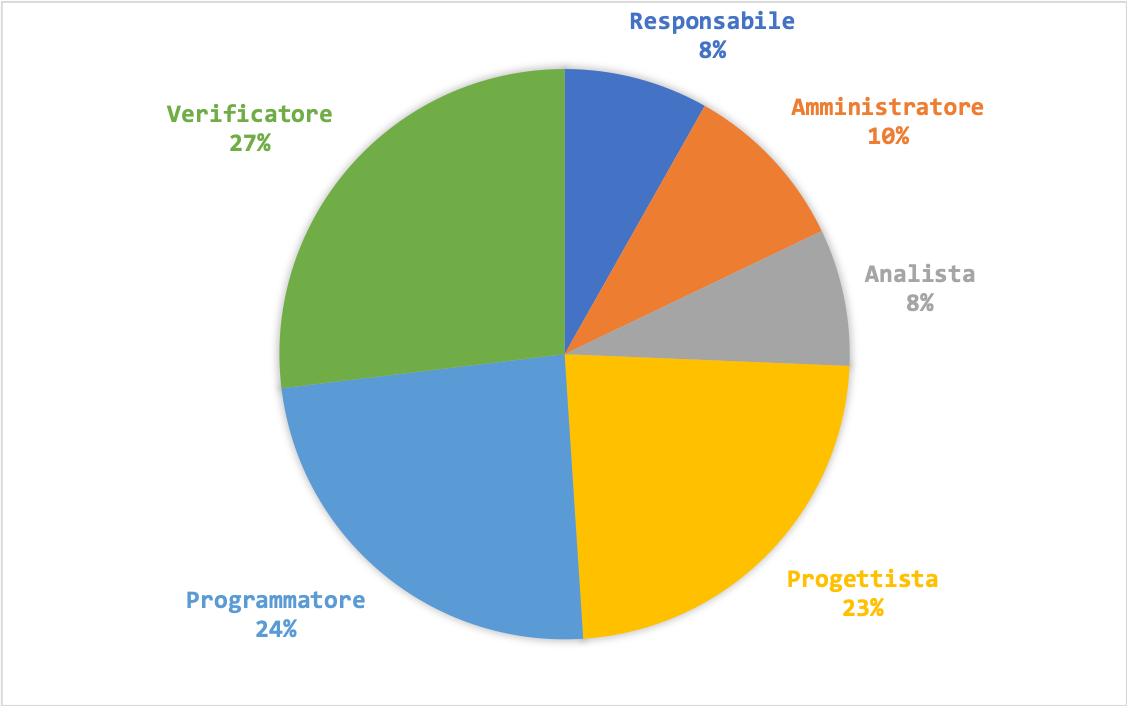
\includegraphics[width=0.8\linewidth]{./images/preventivo/totOreRed2.png}
			\caption{Diagramma percentuale ore/ruolo nel totale delle ore rendicontate}
			\label{fig:diagramma costi ruolo fase totale ore rendicontate}
		\end{figure}
		
		\pagebreak
		
		\subsection{Conclusioni}
		Il progetto si è concluso in modo positivo e il gruppo può ritenersi soddisfatto sia del prodotto ottenuto, sia del metodo con cui sono state gestite le risorse e di come questo abbia portato al raggiungimento di tutti gli obiettivi prefissati. Nonostante le difficoltà iniziali nel redigere una buona pianificazione, il gruppo è riuscito, modificandola e raffinandola più volte nel corso del progetto, a rispettare tutte le scadenze e tutti i costi prestabiliti. Tali difficoltà sono state principalmente causate dalla mancanza di esperienza, fattore fondamentale per organizzare compiti e ruoli in modo adeguato per un progetto di questa durata.
		\newline
		Uno dei fattori fondamentali che ha permesso il raggiungimento di questo risultato è stata l'ottima collaborazione tra tutti i componenti del gruppo. Questo ha fatto sì che la comunicazione tra membri che ricoprivano ruoli diversi fosse sempre precisa e puntuale, consentendo la cooperazione necessaria per la risoluzione dei problemi che si sono verificati durante le varie fasi di sviluppo, senza però causare inefficienze in termini di tempo.
		\newline
		Sebbene la pianificazione finale si sia rivelata sufficientemente matura da permettere al gruppo di concludere lo sviluppo nei tempi previsti, non si è dimostrata del tutto adeguata nella gestione dei rischi non preventivati, situazione che si è infine concretizzata nell'ultima fase. Nello specifico, in seguito alla segnalazione dei committenti, è stato necessario apportare ingenti modifiche a contenuto e struttura del manuale utente, quando le attività previste comprendevano solo l'aggiunta delle nuove funzionalità sviluppate. In tale circostanza, infatti, gli sforzi di ottimizzazione dei componenti del gruppo non sono bastati ad evitare un costo negativo a consuntivo; tuttavia questa perdita è stata bilanciata dal risparmio accumulato nelle fasi precedenti, a riprova del fatto che in mancanza di imprevisti la pianificazione è stata efficace.
		\newline
		In generale, uno degli obiettivi principali del team è stato cercare di suddividere molto finemente le fasi di sviluppo, in modo da poter avere un maggior controllo sul consumo di risorse, limitando le azioni correttive. Questo ha permesso di contenere il numero di ore di responsabile e di amministratore man mano che lo sviluppo avanzava. In compenso, la complessità del sistema da implementare ed il numero delle sue componenti ha costretto i programmatori a mantenere alto il ritmo di codifica e questo, combinato con i tempi serrati, ha richiesto nel lungo termine un aumento delle ore di lavoro. Conseguentemente è stato necessario dedicare più tempo anche alle attività di verifica. 
		\newline\newline
		Al termine delle attività di progetto, il costo totale per lo sviluppo del prodotto ammonta a € 13.786,00, pareggiando il preventivo.
				
		%=================================================================%
		
%	 	\subsection{Tabella riassuntiva del preventivo a finire}
%	 		Di seguito il confronto tra preventivo e consultivo per le varie fasi:
%			 \rowcolors{2}{white}{lightest-grayest}
%			 \begin{longtable}{|l|c|c|c|}
%			 	\hline
%			 	\rowcolor{lighter-grayer}
%			 	\textbf{Fase} & \textbf{Preventivo in €} & \textbf{Consuntivo in €} & \textbf{Differenza in €}\\
%			 	\hline
%				\endfirsthead
%			 	
%			 	\hline
%			 	Analisi & 4.430,00 & 4.410,00 & -20,00\\
%			 	\hline
%			 	\hline
%			 	Consolidamento dei requisiti & 730,00 & 735,00 & +5,00\\
%			 	\hline
%			 	\hline
%			 	Technology baseline & 2.006,00 & 1.991,00 & -15,00\\
%			 	\hline
%			 	\hline
%			 	Incremento I & 701,00 & 689,00 & -12,00\\
%			 	\hline
%			 	\hline
%			 	Incremento II & 813,00 & 810,00 & -3,00\\
%			 	\hline
%			 	\hline
%			 	Incremento III & 774,00 & 788,00 & 14,00\\
%			 	\hline
%			 	\hline
%			 	Incremento IV & 833,00 & 819,00 & -14,00\\
%			 	\hline
%			 	\hline
%			 	Incremento V & 772,00 & 801,00 & +29,00\\
%			 	\hline
%			 	\hline
%			 	Incremento VI & 884,00 & 884,00 & -\\
%			 	\hline
%			 	\hline
%			 	Incremento VII & 747,00 & 740,00 & -7,00\\
%			 	\hline
%			 	\hline
%			 	Incremento VIII & 768,00 & 761,00 & -7,00\\
%			 	\hline
%			 	\hline
%			 	Incremento IX & 777,00 & 777,00 & -\\
%			 	\hline
%			 	\hline
%			 	Incremento X & 782,00 & 782,00 & -\\
%			 	\hline
%			 	\hline
%			 	Incremento XI & 740,00 & 747,00 & +7\\
%			 	\hline
%			 	\hline
%			 	Incremento XII & 1.224,00 & 1.224,00 & -\\
%			 	\hline
%		 		\hline
%			 	Validazione e collaudo & 2.139,00 & 2.147,00 & +8,00\\
%			 	\hline
%			 	\textbf{Totale rendicontato} & 13.786,00 & 13.786,00 & -\\
%			 	\hline
%			 	\hline
%			 	\textbf{Totale} & 18.946,00 & 18.931,00 & -15,00\\
%			 	\hline
%			 	\caption{Tabella contenente il preventivo a finire}
%			 \end{longtable}
